% ============================================================
% 第7章 理論モデルに基づくシミュレーション分析
% ============================================================

% ------------------------------------------------------------
% ・理論モデル（第4章）で導出した構造を可視化する
% ・Z_lin を用いて倒産確率の挙動を確認する
% ・実証分析（第7章）に入る前の理論的整合性を示す
% ------------------------------------------------------------

\chapter{理論モデルに基づくシミュレーション分析}
\label{chap:simulation}

本章は，第6章で構築した実証データを用いる前段階として，
第4章・第5章で導出した理論モデルの挙動を数値的に確認し，
第8章・第9章で行う実証分析につながる理論的基盤を整えることを目的とする。

% ------------------------------------------------------------
% 7.1 本章の目的と位置づけ
% ------------------------------------------------------------


\section{本章の目的と位置づけ}

本章では，第4章・第5章で導出した Merton 型の連続時間モデルの構造を踏まえつつ，
その挙動を離散的なグリッド上で数値的に確認することで，
理論編と実証編を接続する役割を担う。
すなわち，本章は「連続時間モデルに基づく離散化シミュレーション」を通じて，
連続的な潜在倒産距離の含意を整理し，
第8章の潜在倒産距離モデルおよび第9章の Ordered Logit 推定における
係数符号や cutpoint の解釈を容易にするための理論的基盤を整える。

この構成により，本章は
（1）理論モデルの符号条件を数値的に検証する段階，
（2）連続的潜在変数を離散的な実証モデルへ写像する準備段階，
（3）実証分析における係数符号・cutpoint の解釈を補助する段階
として機能する。

さらに，本章では，第6章で整備した新電力企業の財務データおよび市場データの構造を踏まえ，
倒産距離の四要素（収益性 $\mu$，市場ショック感応度 $\sigma$，支援能力 $S$，
負債比率 $D$）が倒産確率にどのような影響を与えるかを体系的に検証する。
具体的には，本章は以下の二つの目的を統合的に扱う。

\begin{itemize}
    \item 理論モデルが示す倒産確率の構造的特徴を可視化すること（第7.1〜7.4節）
    \item Bharath \& Shumway（2008）のロジット式に基づき，
          新電力企業の代表パターンごとの倒産確率を算出し，
          Merton 型シミュレーションとの整合性を確認すること（第7.5節）
\end{itemize}

加えて，本研究ではこれらの分析を補完するために，
\textbf{proxy 変数（A〜D）の精度が推定係数や倒産確率の識別性能に与える影響を，
理想化された世界（真の係数・真の倒産確率が既知）で体系的に評価する
proxy 妥当性シミュレーションを実施する}。
この分析は measurement error 文献の理論を倒産モデルの文脈に応用したものであり，
\textbf{本研究の独創的な成果のひとつ}である。
詳細な導出過程および追加図表は付録Cに整理して示す。

これらの分析は，倒産研究の先行文献および統計学の測定誤差研究に位置づけられ，
第6章で構築した財務データの構造が倒産確率に与える影響を直感的に理解するための
基礎を提供する。
以下では，まず線形倒産距離の理論的背景を整理したうえで，
理論モデルに基づく可視化分析（7.1〜7.4）と，
B\&S 型倒産確率の構造分析（7.5）を順に示す。


% ------------------------------------------------------------
% 7.2 線形倒産距離を用いる正当性
% ・Merton の厳密式を使わず Z_lin を使う理由を説明する節
% ・B&S の proxy DD との構造的類似性を強調
% ------------------------------------------------------------

\section{線形倒産距離を用いる正当性}

本研究で線形倒産距離 $Z_{\text{lin}}$ を用いる第一の理由は、
Merton（1974）モデルの厳密な倒産距離（Distance to Default: DD）が、
新電力企業のデータ環境において実務的に推計不可能であるためである。
Merton モデルは企業価値 $V$ とそのボラティリティ $\sigma_V$ を前提とするが、
これらは市場で直接観測されない。
特に新電力企業は非上場企業が多く、株価データが存在しない場合も多い。
また、負債の時価評価や満期構造の単純化といった仮定も現実の財務構造と乖離しており、
厳密 DD をそのまま適用することは現実的ではない。
したがって、観測可能な財務データのみを用いて倒産リスクを評価できる指標が必要となる。

第二に、Bharath and Shumway（2008）は、
Merton モデルの構造を保ちながら観測可能変数のみで推計可能な
proxy DD（線形化 DD）を提案しており、
その予測性能は厳密 DD と同等、あるいはそれ以上であることが示されている。
後続研究（Tinoco and Wilson, 2013 など）でも同様の結果が確認されており、
線形化された倒産距離は実証研究において広く採用されている。
本研究で用いる $Z_{\text{lin}}$ は、この proxy DD の構造を理論的に整理し直したものであり、
Merton モデルの基本的な符号条件
（収益性の上昇は倒産リスクを低下させ、ボラティリティの上昇は倒産リスクを高める等）
を忠実に保持している。

第三に、新電力企業のリスク構造は $Z_{\text{lin}}$ の構成要素と整合的である。
収益性 $\mu$ はキャッシュフローの持続可能性を反映し、
市場ショック $\sigma$ はスポット価格の急騰・急落といった外生ショックを捉える。
支援能力 $S$ は親会社やスポンサー企業による財務支援の強さを表し、
負債比率 $D$ は財務的脆弱性を直接的に示す。
これら 4 つの要因は、新電力企業の倒産事例で繰り返し指摘されてきた主要なリスク要因と一致しており、
$Z_{\text{lin}}$ は新電力の倒産リスクを構造的に捉える指標として適切である。

以上より、$Z_{\text{lin}}$ を用いることは、
データ制約の大きい新電力企業に対して理論的にも実証的にも妥当であり、
本章のシミュレーション分析において適切なアプローチである。

\subsection{連続モデル（理論）と離散モデル（実証）の関係}

本章で扱う Merton 型倒産モデルおよび B\&S 型ロジット式は，
倒産確率を連続的な潜在変数（倒産距離 $Z_{\text{lin}}$）として扱う点に特徴がある。
すなわち，倒産確率は


\[
p = \Lambda(-Z_{\text{lin}})
\]


のように連続的に変化し，倒産は「確率が高まる連続的な現象」として記述される。

一方，第9章で実施する Ordered Logit 推定では，
倒産は


\[
\text{stage} \in \{0,1,2\}
\]


という離散的な段階として観測される。
これは，実データでは倒産確率そのものが観測できず，
倒産の発生形態（存続・財務悪化・倒産）だけが観測可能であるためである。

したがって，本研究では
\begin{itemize}
    \item 第7章：連続的倒産距離の構造を理論的に理解する段階
    \item 第8章：連続的倒産距離を潜在変数 $y^*$ に写像する段階
    \item 第9章：潜在変数が閾値を跨ぐことで離散的倒産ステージが生成される段階
\end{itemize}
という三段階構造を採用している。

この構造は Ordered Logit モデルの本質と完全に整合しており，
連続モデルと離散モデルの間に不整合は存在しない。
むしろ，連続モデルの挙動を本章で可視化しておくことで，
第9章の実証分析における係数符号・cutpoint の解釈が容易となる。


% ============================================================
% 7.3 限界と注意点
% ・Z_lin を用いた分析の前提条件と限界を明示する
% ・第7章の実証分析に向けた注意点を整理する
% ============================================================

\section{限界と注意点}

本節では、線形倒産距離 $Z_{\text{lin}}$ を用いたシミュレーション分析に伴う
理論的・実務的な限界について整理する。
これらの点を明確にすることで、本章の分析結果をどの範囲で解釈すべきかを示し、
第7章の実証分析に向けた前提条件を明確化する。

第一に、$Z_{\text{lin}}$ は Merton（1974）モデルの厳密な倒産距離を
線形化した近似指標であり、資産価値の確率過程や負債構造に関する
Merton モデル固有の仮定を簡略化している。
特に、資産価値が幾何ブラウン運動に従うという仮定や、
負債が単一満期の割引債として扱われるという前提は、
現実の企業財務構造と必ずしも一致しない。
したがって、$Z_{\text{lin}}$ は倒産リスクの方向性を捉える指標としては有効であるものの、
絶対水準の精緻な推計を目的とするものではない。

第二に、本研究で設定したパラメータ
（収益性 $\mu$、市場ショック $\sigma$、支援能力 $S$、負債比率 $D$）
は、新電力企業の典型的な財務特性を反映したものであるが、
すべての企業の実態を完全に表現するものではない。
特に新電力企業は、スポット市場価格の急変動や需給調整金の増減といった
外生ショックの影響を強く受けるため、
$\sigma$ の変動幅は時期によって大きく異なる。
また、支援能力 $S$ は親会社の財務基盤や支援方針に依存するため、
離散的な段階化によって完全に表現できるわけではない。

第三に、$Z_{\text{lin}}$ は財務データに基づく静学的な指標であり、
企業行動や市場制度の変化を内生的に取り込むものではない。
新電力企業の倒産リスクは、燃料価格の高騰、制度変更、
広域機関による需給調整ルールの改定など、
制度的・政策的要因によって大きく左右される。
これらの要因は本章のシミュレーションには直接的には反映されていないため、
$Z_{\text{lin}}$ による倒産確率は、あくまで
「財務構造と市場ショックに基づく基礎的なリスク水準」
を示すものとして解釈する必要がある。

以上の点を踏まえると、本章のシミュレーションは
新電力企業の倒産リスクの構造的特徴を理解するうえで有用である一方、
制度変更や市場環境の急激な変化を伴う状況においては、
追加的な分析や補正が必要となる。
次章では、これらの限界を踏まえつつ、
実際の財務データを用いた実証分析を行い、
$Z_{\text{lin}}$ の有効性と現実的な適用可能性を検証する。

% ============================================================
% 7.4 4変数の独立性に関する前提とその正当化
% ------------------------------------------------------------
% ・μ・σ・S・D を独立とみなす前提の根拠を明示する節
% ・7.3 のシミュレーション設定に入る前の理論的前提を補強
% ============================================================

\section{4変数の独立性に関する前提とその正当化}

本研究では，倒産確率を規定する主要因として，収益性（$\mu$），外部ショック感応度（$\sigma$），支援能力（$S$），倒産閾値（$D$）の4変数を設定し，これらを相互依存を前提としない独立の説明変数として扱う。この前提は以下の理由から正当化される。

第一に，$\mu$・$\sigma$・$S$・$D$ は，Merton（1974）型の構造モデルおよび Bharath and Shumway（2008）の倒産確率モデルにおいて，異なる経済的メカニズムから導出される概念的に独立したパラメータである。具体的には，$\mu$ は企業価値のドリフト（収益性），$\sigma$ は企業価値のボラティリティ（外部ショック感応度），$D$ は負債構造に基づく倒産閾値，$S$ は親会社・金融機関等による外生的支援能力を表す。これらはモデル内部で異なる役割を担うため，構造的に独立した変数として扱うことが理論的に整合的である。

第二に，4変数は異なる主体・異なる意思決定プロセスによって決定されるため，経済学的にも相互依存を前提としないことが合理的である。$\mu$ は企業の経営努力や事業構造に依存する内生的要因である一方，$\sigma$ は市場価格（JEPX）や制度変更といった外生的ショックにより規定される。$S$ は親会社・金融機関等の支援姿勢に依存し，$D$ は負債構造や制度的要件によって決まる。このように，決定主体が異なるため，4変数を独立の説明変数として扱うことは経済学的に妥当である。

第三に，実証分析の観点からも，相互依存を前提としないことは合理的である。倒産研究におけるロジット推定の目的は，各変数が倒産確率に与える符号条件の妥当性を確認することであり，変数間の因果連鎖を精緻にモデル化することではない。特に本研究のようにサンプル数が限定される場合，相互依存を前提とした複雑なモデルを構築すると，多重共線性や推定の不安定性を招く。したがって，$\mu$・$\sigma$・$S$・$D$ を独立変数として扱うことは，理論的整合性と実証的安定性の双方を確保するために適切である。

以上より，本研究において $\mu$・$\sigma$・$S$・$D$ を独立の説明変数として扱う前提は，理論的・経済学的・実証的観点から十分に正当化される。





% ============================================================
% 7.5 シミュレーションの設定（強化版）
% ============================================================

\section{シミュレーションの設定}

本節では、第4章で導出した潜在倒産距離 $Z_{\text{lin}}$ を用いて、
倒産確率の挙動を体系的に評価するためのシミュレーション設定を明確化する。
ここで示す設定は、理論モデルの符号条件
（$\mu$ の上昇は倒産リスクを低下させ、$\sigma$ の上昇は倒産リスクを高める等）
が数値的にどのように現れるかを可視化するための基礎となる。

なお，本節で設定する離散的なパラメータ範囲は，連続時間モデルを数値的に扱うための
離散化（discretization）であり，第9章で用いる離散時間モデルそのものを
定義するものではない\footnote{
本章で用いる離散化（discretization）は，連続時間モデルを数値的に扱うための
便宜的な近似手法であり，離散時間モデル（例えば Ordered Logit）の理論的定義とは
異なる概念である。具体的には，連続的な潜在倒産距離 $Z_{\text{lin}}$ を
グリッド上で評価するために，$\mu$ と $\sigma$ を連続範囲で離散化し，
$S$ と $D$ を代表的なカテゴリに区分している。
これは連続モデルの挙動を可視化するための数値計算上の手続きであり，
離散時間モデルの構造（潜在変数 $y^*$ が閾値を跨ぐことで離散的ステージが生成される）
を定義するものではない。
したがって，本章の離散化は「連続→離散→実証」という本研究の三段階構造のうち，
連続モデルを実証分析へ橋渡しするための補助的な近似計算として位置づけられる。
}.




\subsection*{潜在倒産距離の定義}

潜在倒産距離は、収益性・市場ショック・支援能力・負債比率という
4 つの主要因を線形に統合した次式で与えられる。


\[
Z_{\text{lin}} = \mu - \sigma + S - D
\]


この構造は Bharath and Shumway（2008）の proxy DD と同様に、
Merton モデルの基本的な符号条件を保持しつつ、
観測可能な財務データのみで倒産リスクを評価できる点に特徴がある。

\subsection*{倒産確率のロジット写像}

倒産確率は、潜在倒産距離をロジット関数に写像することで定義する。


\[
p = \frac{1}{1 + \exp(-Z_{\text{lin}})}
\]


この写像により、$Z_{\text{lin}}$ が大きくなるほど倒産確率が滑らかに低下し、
逆に $Z_{\text{lin}}$ が負方向に大きくなるほど倒産確率が急速に上昇する。
これは、倒産リスクが連続的かつ非線形に変化するという
実務的な直感とも整合的である。

\subsection*{パラメータ範囲の設定}

シミュレーションでは、新電力企業の典型的な財務特性と市場環境を踏まえ、
以下の範囲でパラメータを設定する。

\begin{itemize}
    \item 収益性：$\mu \in [-0.10, 0.10]$
    \item 市場ショック：$\sigma \in [0.05, 0.50]$
    \item 支援能力：$S \in \{0,1,2,3\}$
    \item 負債比率：$D \in \{0.3, 0.5, 0.8\}$
\end{itemize}

収益性 $\mu$ と市場ショック $\sigma$ は連続的に変化させ、
支援能力 $S$ と負債比率 $D$ は企業類型を反映した離散的な水準を採用する。
これにより、財務構造の違いが倒産確率の地形（surface）にどのような差異を生むかを
明確に比較できる。

\subsection*{設定の意義}

以上の設定により、本章のシミュレーションは以下を可能にする。

\begin{itemize}
    \item 理論モデルの符号条件が数値的にどのように現れるかを可視化する
    \item 支援能力や負債比率の違いが倒産確率の形状に与える影響を明確化する
    \item 第7章の実証分析に向けて、$Z_{\text{lin}}$ の構造的妥当性を事前に検証する
\end{itemize}

これらは、理論と実証を橋渡しするうえで不可欠なステップであり、
本章のシミュレーション設定はその基盤を提供する。

% ============================================================
% 7.6 変数間の相互関係を考慮したシミュレーション
% ------------------------------------------------------------
% ・μ×σ、S×D などの相互作用が Z_lin に与える影響を理論的に可視化
% ・第8章の実証分析（交差項）につながる橋渡し
% ============================================================

\section{変数間の相互関係を考慮したシミュレーション}

前節では，潜在倒産距離 $Z_{\text{lin}} = \mu - \sigma + S - D$ を構成する
4変数を独立の説明変数として扱い，それぞれの符号条件が倒産確率にどのように反映されるかを確認した。
しかし，実際の倒産過程では，これらの変数が「単独で作用する」だけでなく，
\textbf{複数の要因が同時に変化することで倒産リスクが非線形的に増幅・緩和される}
場合が多い。
そこで本節では，$\mu$・$\sigma$・$S$・$D$ の相互関係が
倒産確率の地形にどのような影響を与えるかを，
相互作用項（interaction）を導入した拡張版の潜在倒産距離を用いて可視化する。

\subsection*{相互作用項を含む潜在倒産距離の拡張}

相互関係を考慮した潜在倒産距離は，以下のように定義する。



\[
Z_{\text{int}} 
= \mu - \sigma + S - D 
+ \gamma_{\mu\sigma} (\mu \cdot \sigma)
+ \gamma_{SD} (S \cdot D)
\]



ここで，
\begin{itemize}
    \item $\gamma_{\mu\sigma}$：収益性と市場ショックの相互作用
    \item $\gamma_{SD}$：支援能力と負債比率の相互作用
\end{itemize}
を表す。
$\gamma_{\mu\sigma}$ は「収益性が高い企業ほどショックに強いか」を，
$\gamma_{SD}$ は「支援能力が高い企業ほど負債過多に耐えられるか」を示す。

本研究では，理論的直感に基づき，



\[
\gamma_{\mu\sigma} < 0,\qquad \gamma_{SD} > 0
\]



を想定する。
すなわち，
\begin{itemize}
    \item 収益性が高いほど，市場ショックの悪影響が緩和される
    \item 支援能力が高いほど，負債比率の悪影響が緩和される
\end{itemize}
という構造を仮定する。

\subsection*{相互作用が倒産確率に与える影響}

相互作用項を含む倒産確率は，以下のロジット写像で与えられる。



\[
p_{\text{int}} = \frac{1}{1 + \exp(-Z_{\text{int}})}
\]



この $p_{\text{int}}$ を用いて，以下の2つの相互関係を可視化する。

\begin{enumerate}
    \item \textbf{収益性 $\mu$ と市場ショック $\sigma$ の相互作用}  
    収益性が高い企業では，$\sigma$ の上昇に対する倒産確率の立ち上がりが緩やかになる。
    逆に，$\mu$ が低い企業では，$\sigma$ の上昇が倒産確率を急激に押し上げる。

    \item \textbf{支援能力 $S$ と負債比率 $D$ の相互作用}  
    支援能力が高い企業では，負債比率 $D$ の上昇が倒産確率に与える悪影響が大幅に緩和される。
    一方，$S=0$ の企業では，$D$ の上昇が倒産確率を急激に押し上げる。
\end{enumerate}

% ------------------------------------------------------------
% 図：μ×σ の相互作用
% ------------------------------------------------------------

\begin{figure}[H]
    \centering
    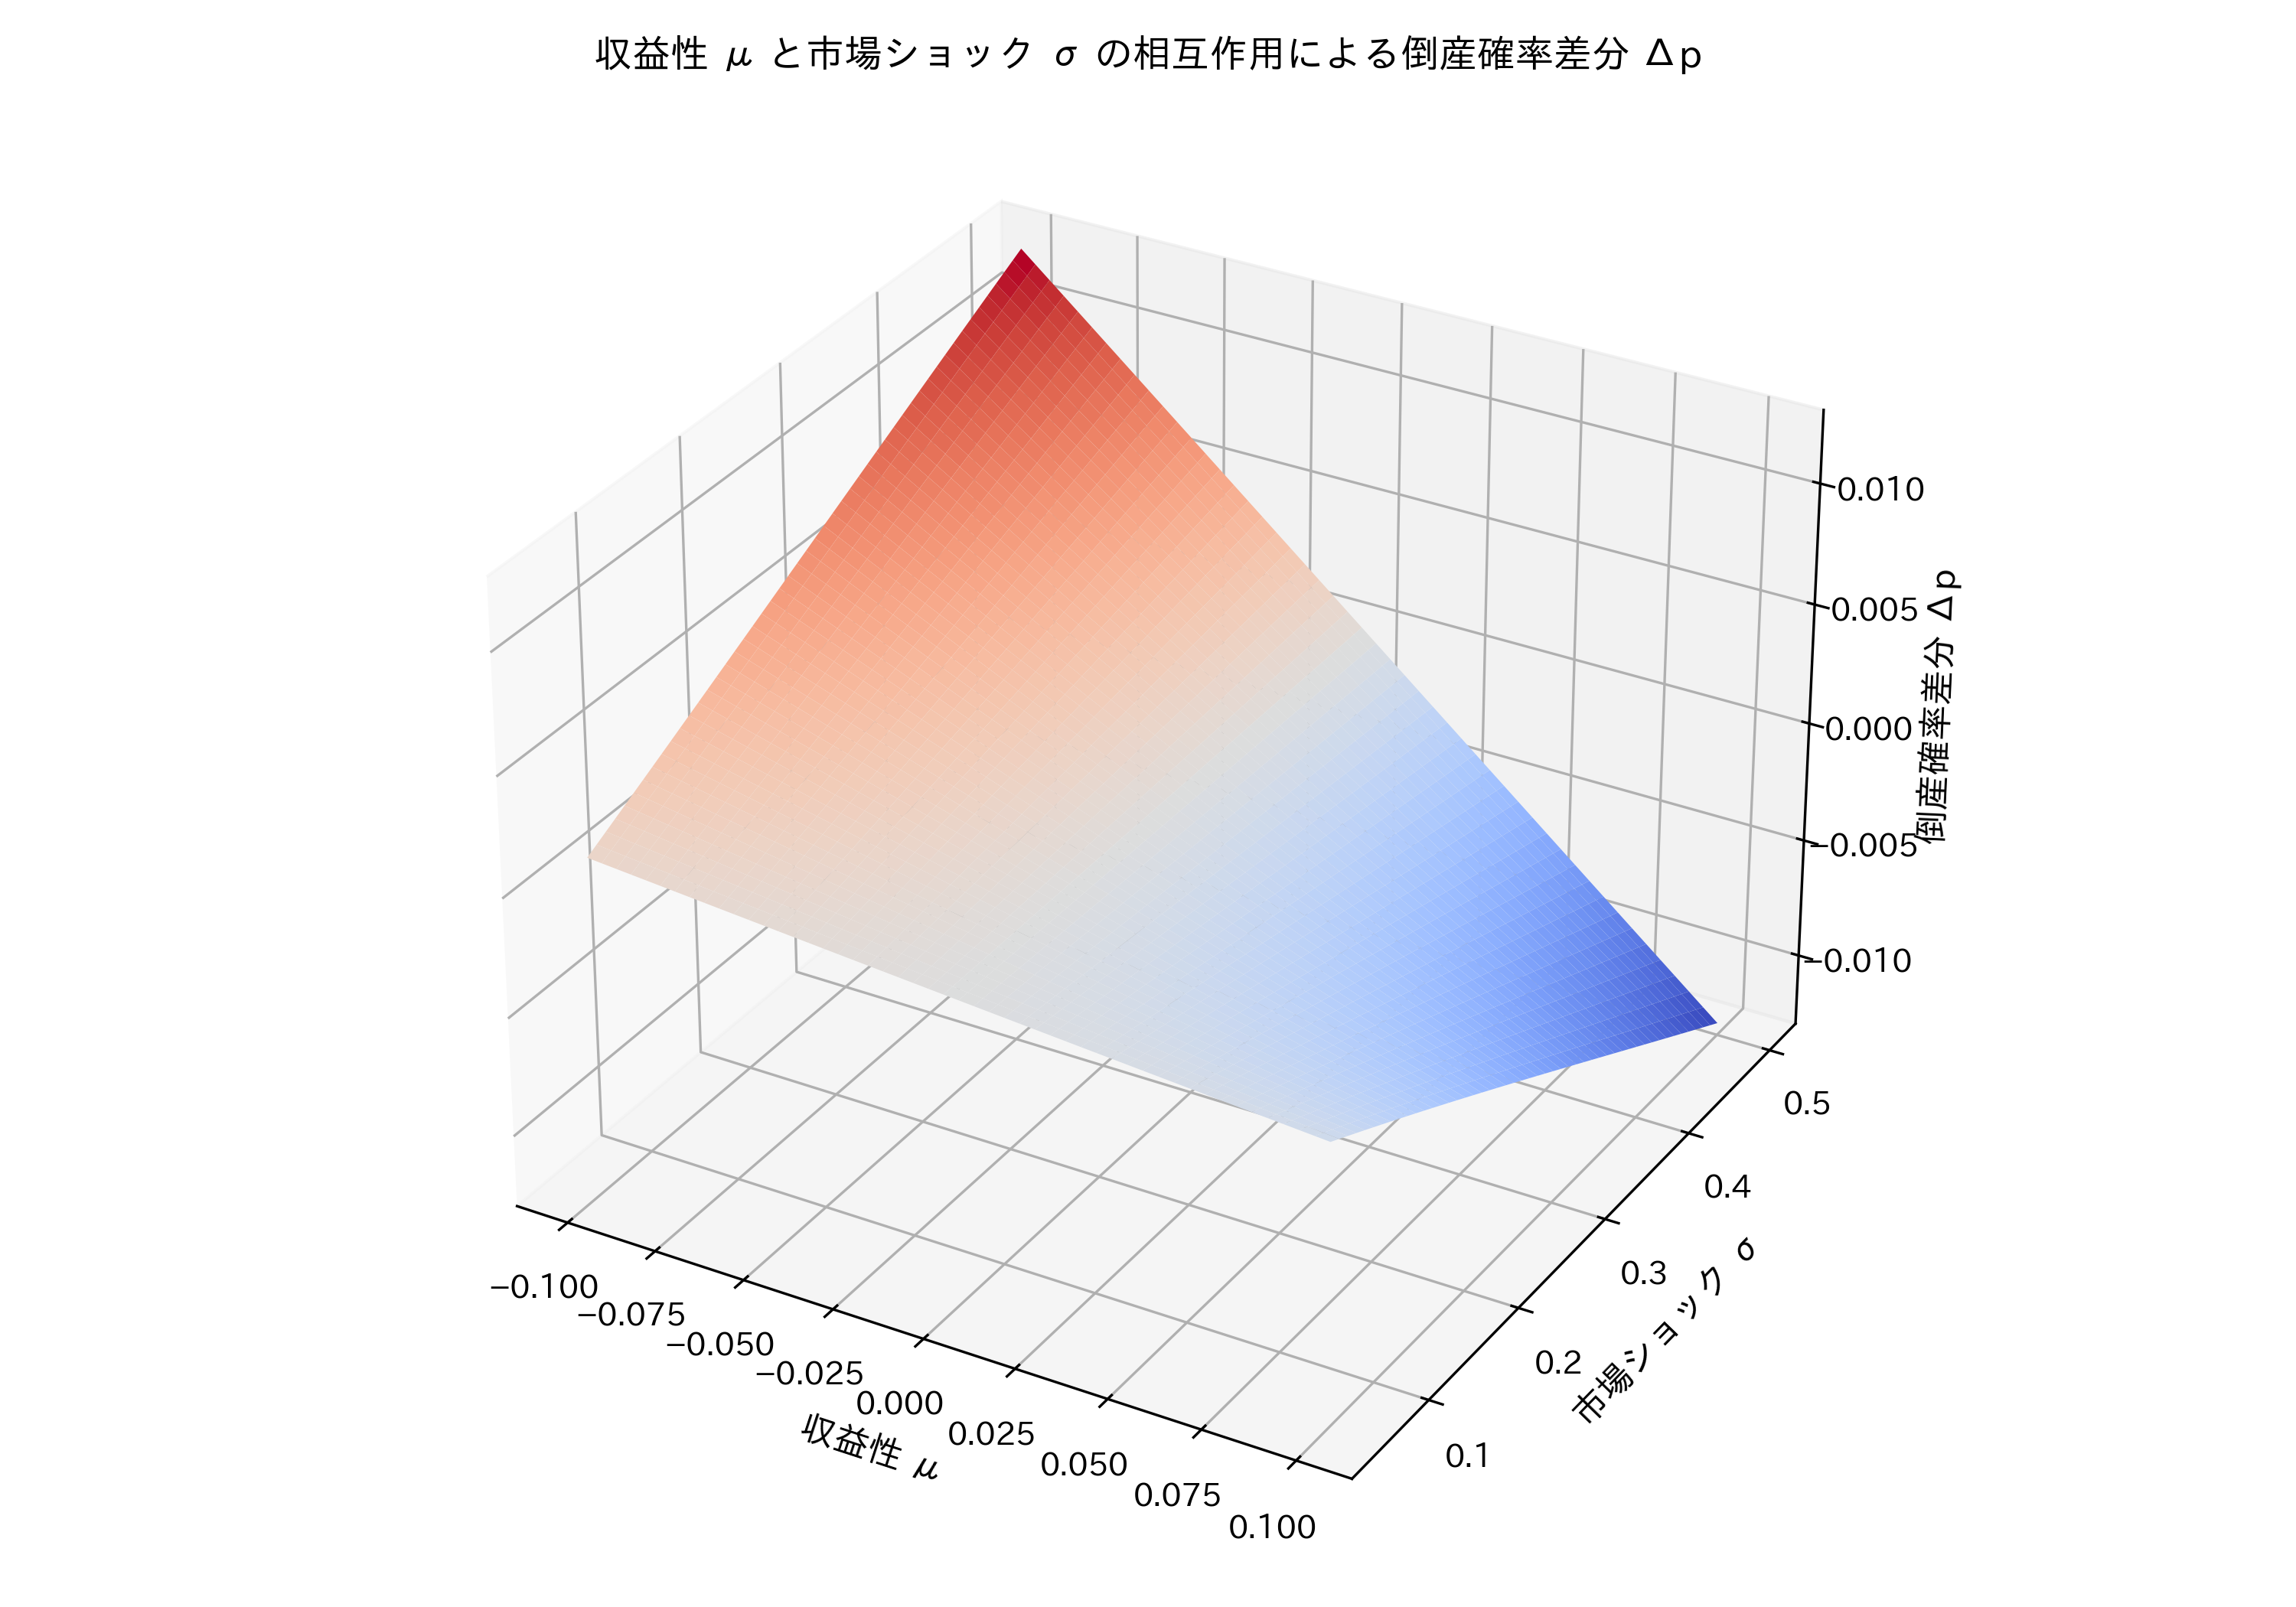
\includegraphics[width=0.80\linewidth]{figures/interaction_mu_sigma_surface.png}
    \caption{収益性 $\mu$ と市場ショック $\sigma$ の相互作用による倒産確率差分 $\Delta p$ の3Dサーフェス}
    \label{fig:interaction_mu_sigma_surface}
\end{figure}

図\ref{fig:interaction_mu_sigma_surface} は，収益性 $\mu$ と市場ショック $\sigma$ の相互作用項
$\gamma_{\mu\sigma}(\mu \cdot \sigma)$ が倒産確率に与える影響を可視化したものである。
相互作用を含む倒産確率 $p_{\mathrm{int}}$ と，相互作用を含まない倒産確率 $p_{\mathrm{base}}$ の差分



\[
\Delta p = p_{\mathrm{int}} - p_{\mathrm{base}}
\]



を3次元サーフェスとして描画している。
$\mu$ が低く $\sigma$ が高い領域で $\Delta p$ が大きくなることから，
収益性が低い企業ほど市場ショックの悪影響が増幅されることが確認できる。
一方，$\mu$ が高い領域では $\sigma$ の影響が緩和され，$\Delta p$ が小さくなる。
これは「収益性がショック耐性を高める」という理論モデルの含意と整合的である。

% ------------------------------------------------------------
% 図：S×D の相互作用
% ------------------------------------------------------------

\begin{figure}[H]
    \centering
    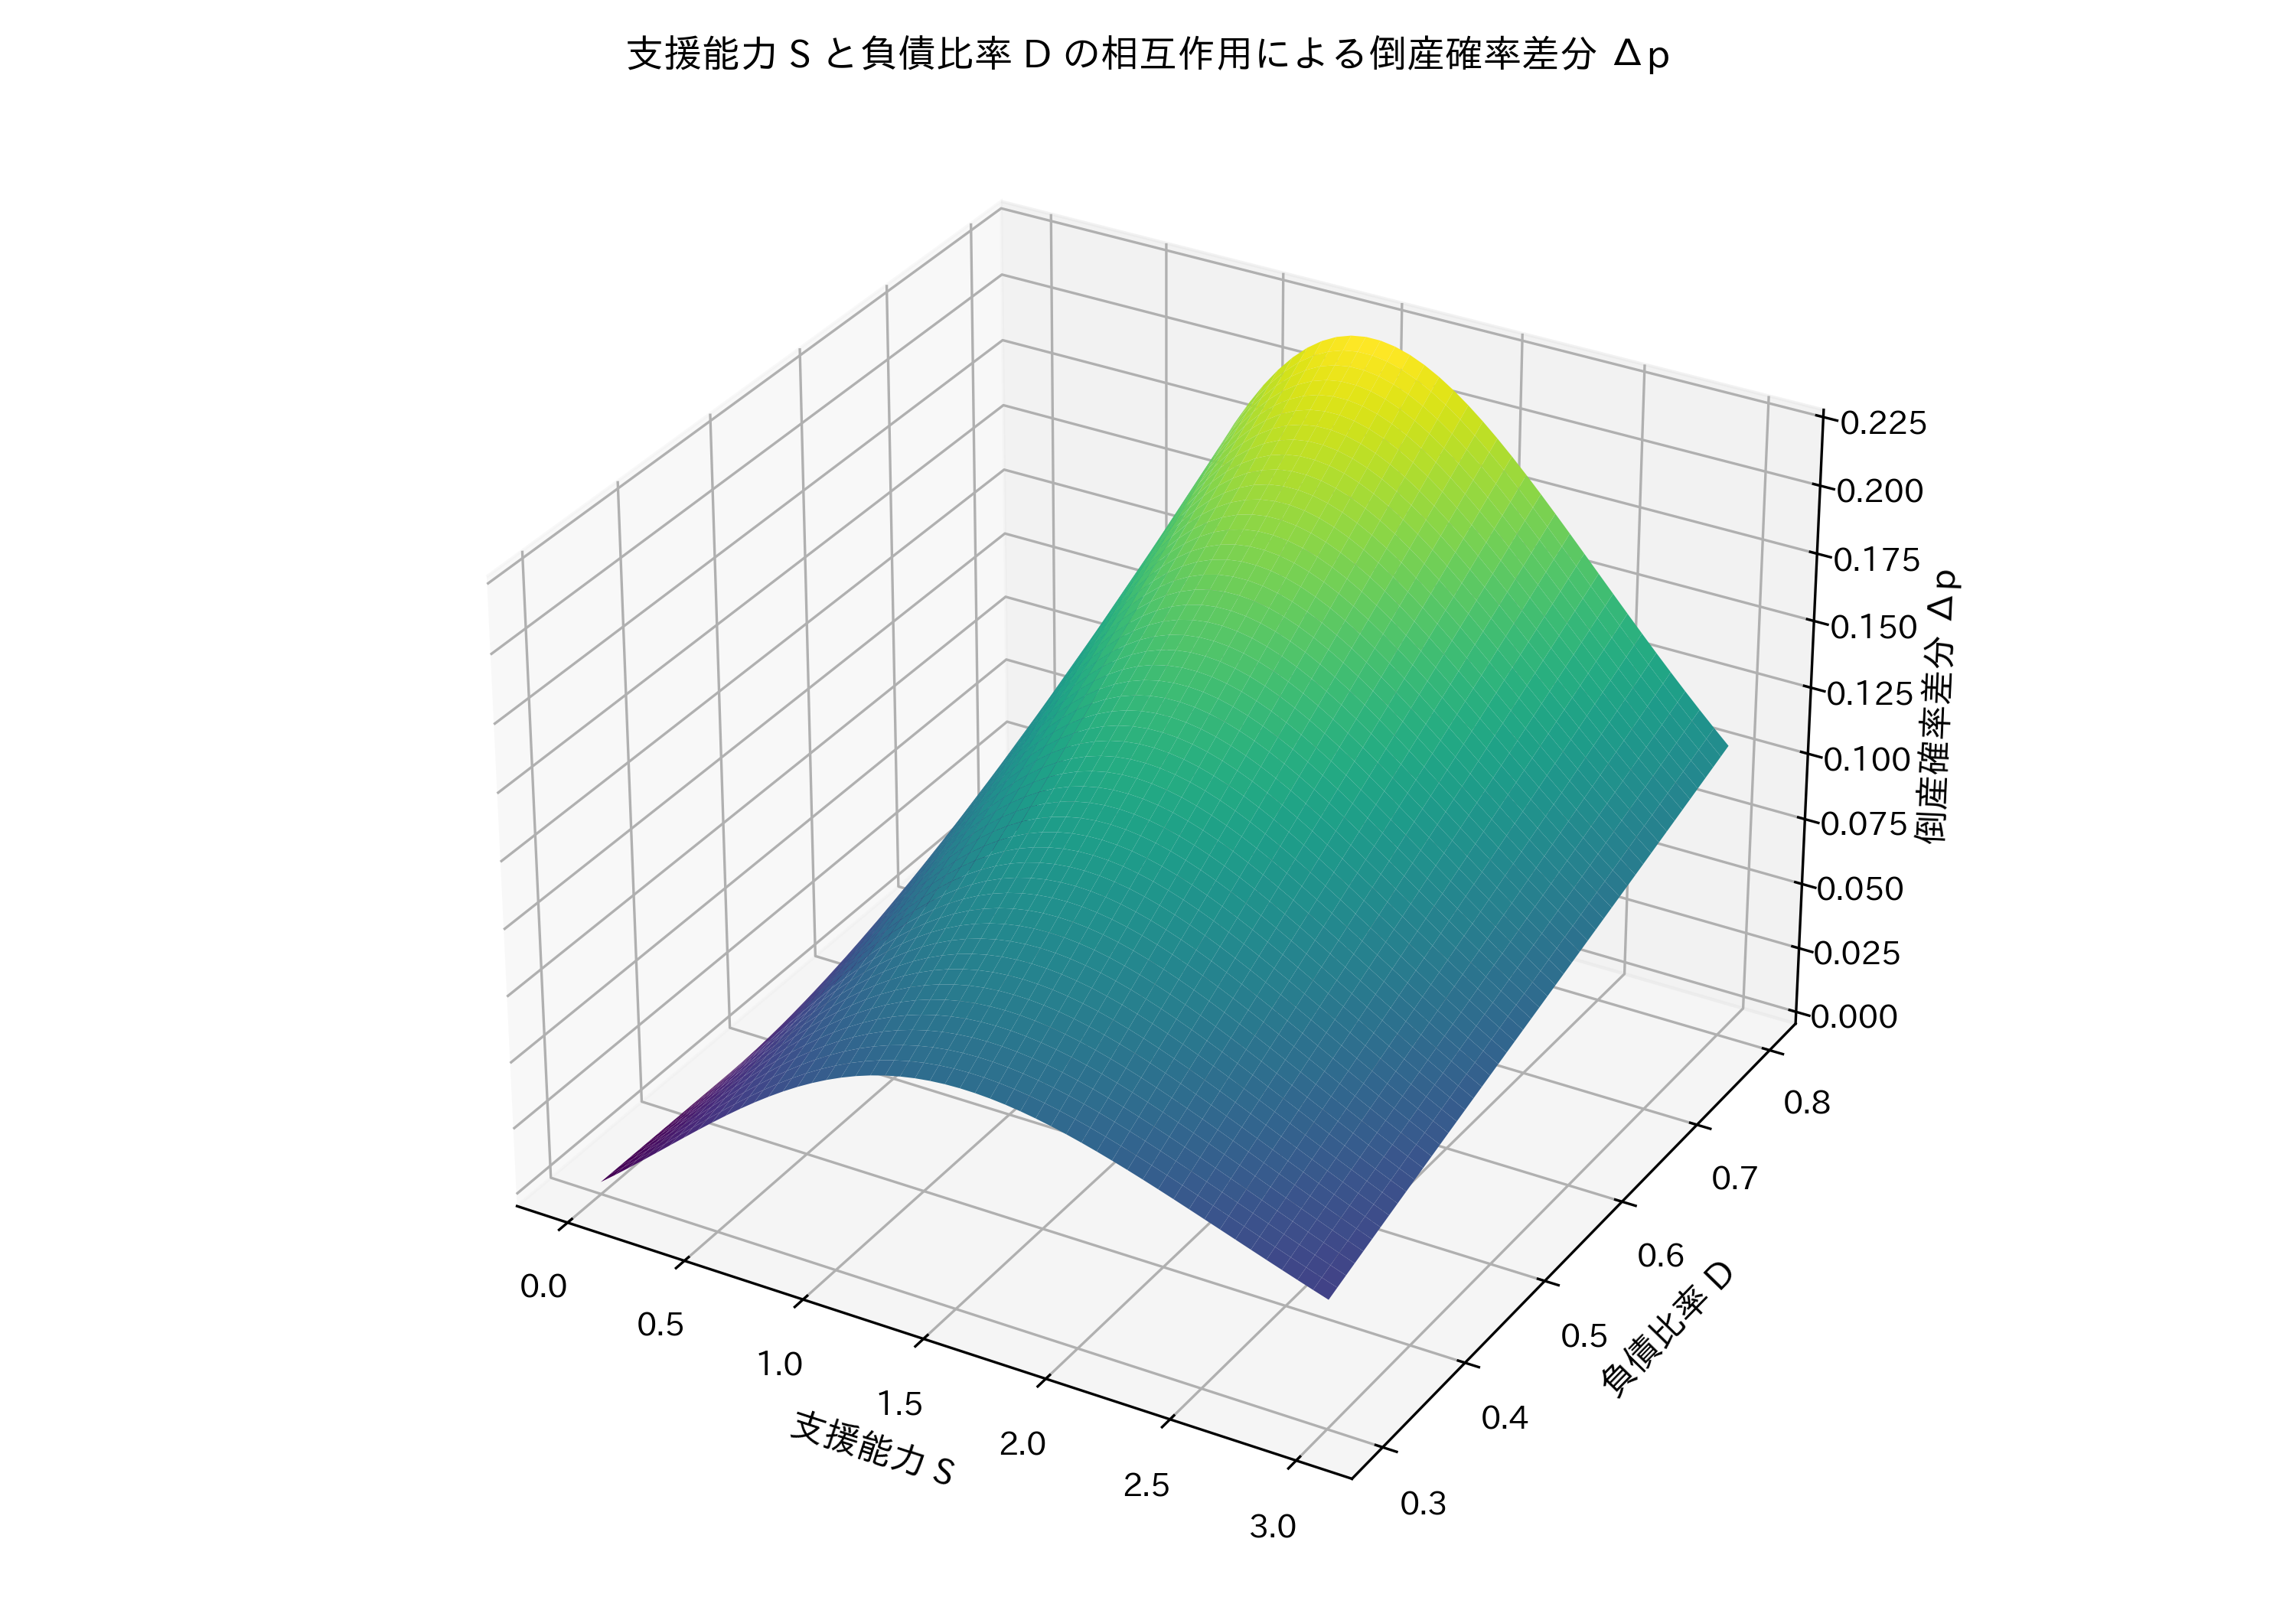
\includegraphics[width=0.80\linewidth]{figures/interaction_S_D_surface.png}
    \caption{支援能力 $S$ と負債比率 $D$ の相互作用による倒産確率差分 $\Delta p$ の3Dサーフェス}
    \label{fig:interaction_S_D_surface}
\end{figure}

図\ref{fig:interaction_S_D_surface} は，支援能力 $S$ と負債比率 $D$ の相互作用項
$\gamma_{SD}(S \cdot D)$ が倒産確率に与える影響を可視化したものである。
相互作用を含む倒産確率と含まない倒産確率の差分



\[
\Delta p = p_{\mathrm{int}} - p_{\mathrm{base}}
\]



を描画している。
$S$ が高い企業では，$D$ の上昇による倒産確率の悪化が大幅に緩和され，
$\Delta p$ が正の plateau（高原）として現れる。
一方，$S=0$ の企業では $D$ の悪影響がそのまま倒産確率に反映され，
$\Delta p$ はほぼゼロとなる。
これは「支援能力が負債過多の悪影響を吸収する」という理論的含意を
数値的に裏付けるものである。

\subsection*{相互関係シミュレーションの意義}

本節の相互関係シミュレーションは，以下の点で重要である。

\begin{itemize}
    \item 第4章の理論モデルで示した「相互作用の符号条件」を数値的に確認できる
    \item 第6.4節の可視化（ケース比較）で観察される非線形性の背景を説明できる
    \item 第8章の実証分析における交差項（$\mu \cdot \sigma$，$S \cdot D$）の導入を理論的に正当化する
\end{itemize}

特に，実証分析ではサンプル数の制約から交差項を 1〜2 個に限定する必要があるが，
本節のシミュレーションにより，
\textbf{どの交差項が倒産確率に最も強く作用するかを事前に把握できる}
点に意義がある。

以上より，本節は理論モデルと実証分析を橋渡しする役割を果たし，
倒産リスクの構造が単一要因ではなく複数要因の相互作用によって決定されることを
数理的に示すものである。



\section{可視化とケース比較}
% ------------------------------------------------------------
% 7.7 可視化とケース比較
% 
% ・ケース設定と3D可視化を統合し、Z_lin の構造を視覚的に確認する
% ・S と D の違いが倒産確率の地形にどう現れるかを体系的に整理する
% ・第7章の実証分析につながる橋渡しの役割を持つ
% ------------------------------------------------------------

本節では，前節で定義した潜在倒産距離


\[
Z_{\text{lin}} = \mu - \sigma + S - D
\]


およびロジット写像


\[
p = \frac{1}{1 + \exp(-Z_{\text{lin}})}
\]


を用いて，新電力企業の倒産確率がどのような地形を描くのかを可視化する。
特に，支援能力 $S$ と負債比率 $D$ が倒産確率の基準水準をどのように規定するのかを，
代表的なケース設定と 3D サーフェスプロットを通じて比較する。

% ============================================================
\subsection{ケース設定}
% ------------------------------------------------------------
% ・企業の典型的な財務状態を6ケースに分類
% ・S と D の組合せが Z_lin の基準水準をどう規定するかを示す
% ・第7章の実証分析で用いる財務プロファイルの基礎分類
% ------------------------------------------------------------

本研究では，新電力企業の典型的な財務状態と資本構造を踏まえ，
倒産リスクの構造的特徴を把握するために，以下の 6 ケースを設定する。
これらは，負債比率 $D$ と支援能力 $S$ の代表的な組合せを体系的に網羅したものであり，
新電力企業の多様な財務プロファイルを抽象化した分類である。

\begin{itemize}
    \item ケースA：$D=0.3,\ S=0$（独立系・財務健全）
    \item ケースB：$D=0.3,\ S=3$（大手系・財務健全）
    \item ケースC：$D=0.8,\ S=0$（独立系・負債過多）
    \item ケースD：$D=0.8,\ S=3$（大手系・負債過多）
    \item ケースE：$D=0.5,\ S=1$（地域新電力）
    \item ケースF：$D=0.5,\ S=2$（商社系）
\end{itemize}

これらのケースは，$Z_{\text{lin}}$ の構造において，
支援能力 $S$ が倒産確率の「底上げ」を行い，
負債比率 $D$ がその逆方向に作用するという基本的な力学を比較するための基盤となる。

% ============================================================
\subsection{3D サーフェスプロットによる可視化}
% ------------------------------------------------------------
% ・μ と σ を連続的に動かし，p の3D地形を描画する
% ・S と D の違いが地形の位置と急峻性にどう現れるかを確認
% ・理論モデルの符号条件が視覚的に再現されることを示す
% ------------------------------------------------------------

本節では，各ケースについて倒産確率 $p$ の 3 次元サーフェスプロットを作成し，
$Z_{\text{lin}}$ の符号条件がどのように地形として現れるかを確認する。
以下では，ケースA〜Fの順に図を示し，それぞれの特徴を簡潔に整理する。

% ---------- ケースA ----------
\subsubsection*{ケースA：$D=0.3,\ S=0$（独立系・財務健全）}

\begin{figure}[H]
    \centering
    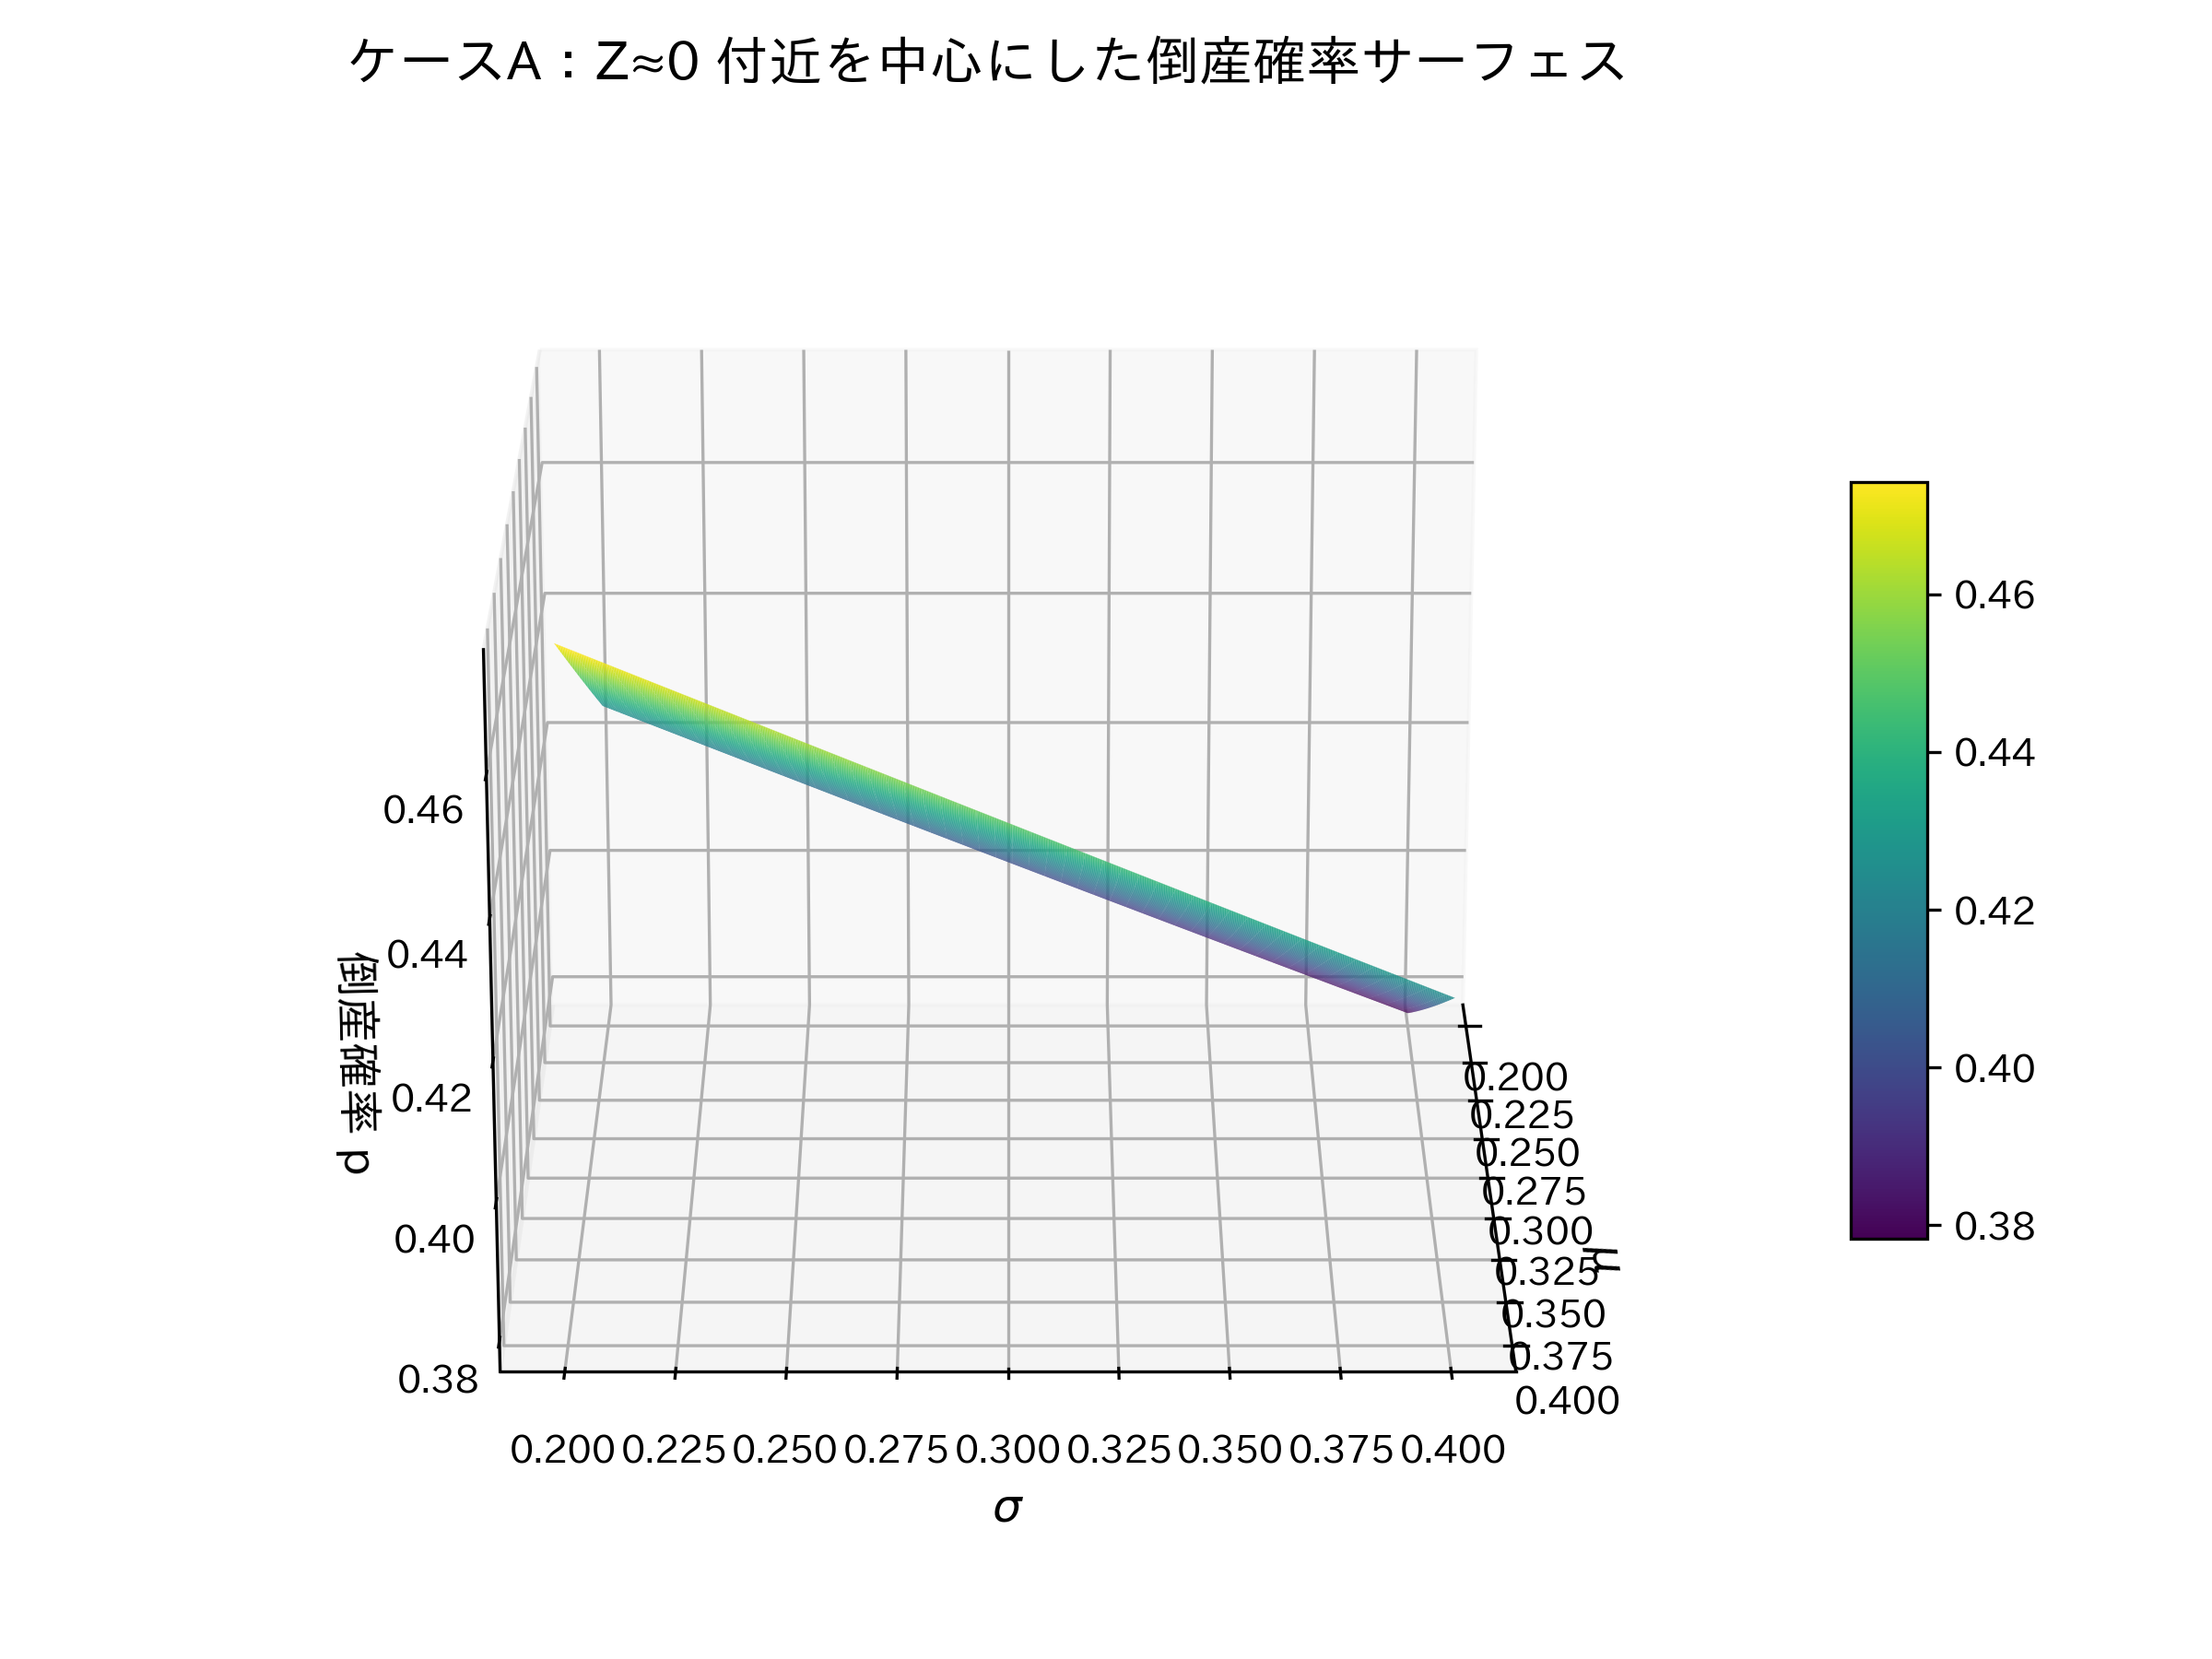
\includegraphics[width=0.75\linewidth]{figures/surface_caseA_centered.png}
    \caption{ケースAにおける倒産確率の3Dサーフェスプロット（Z≈0付近を中心）}
    \label{fig:surface_caseA_centered}
\end{figure}

ケースAでは，支援能力がなく負債比率も低いため，
倒産確率の基準水準は比較的低い。
Z≈0 付近を中心に描画することで，
$\sigma$ の上昇に対する急峻な立ち上がりがより明確に示され，
外生ショックへの脆弱性が視覚的に強調される。


% ---------- ケースB ----------
\subsubsection*{ケースB：$D=0.3,\ S=3$（大手系・財務健全）}

\begin{figure}[H]
    \centering
    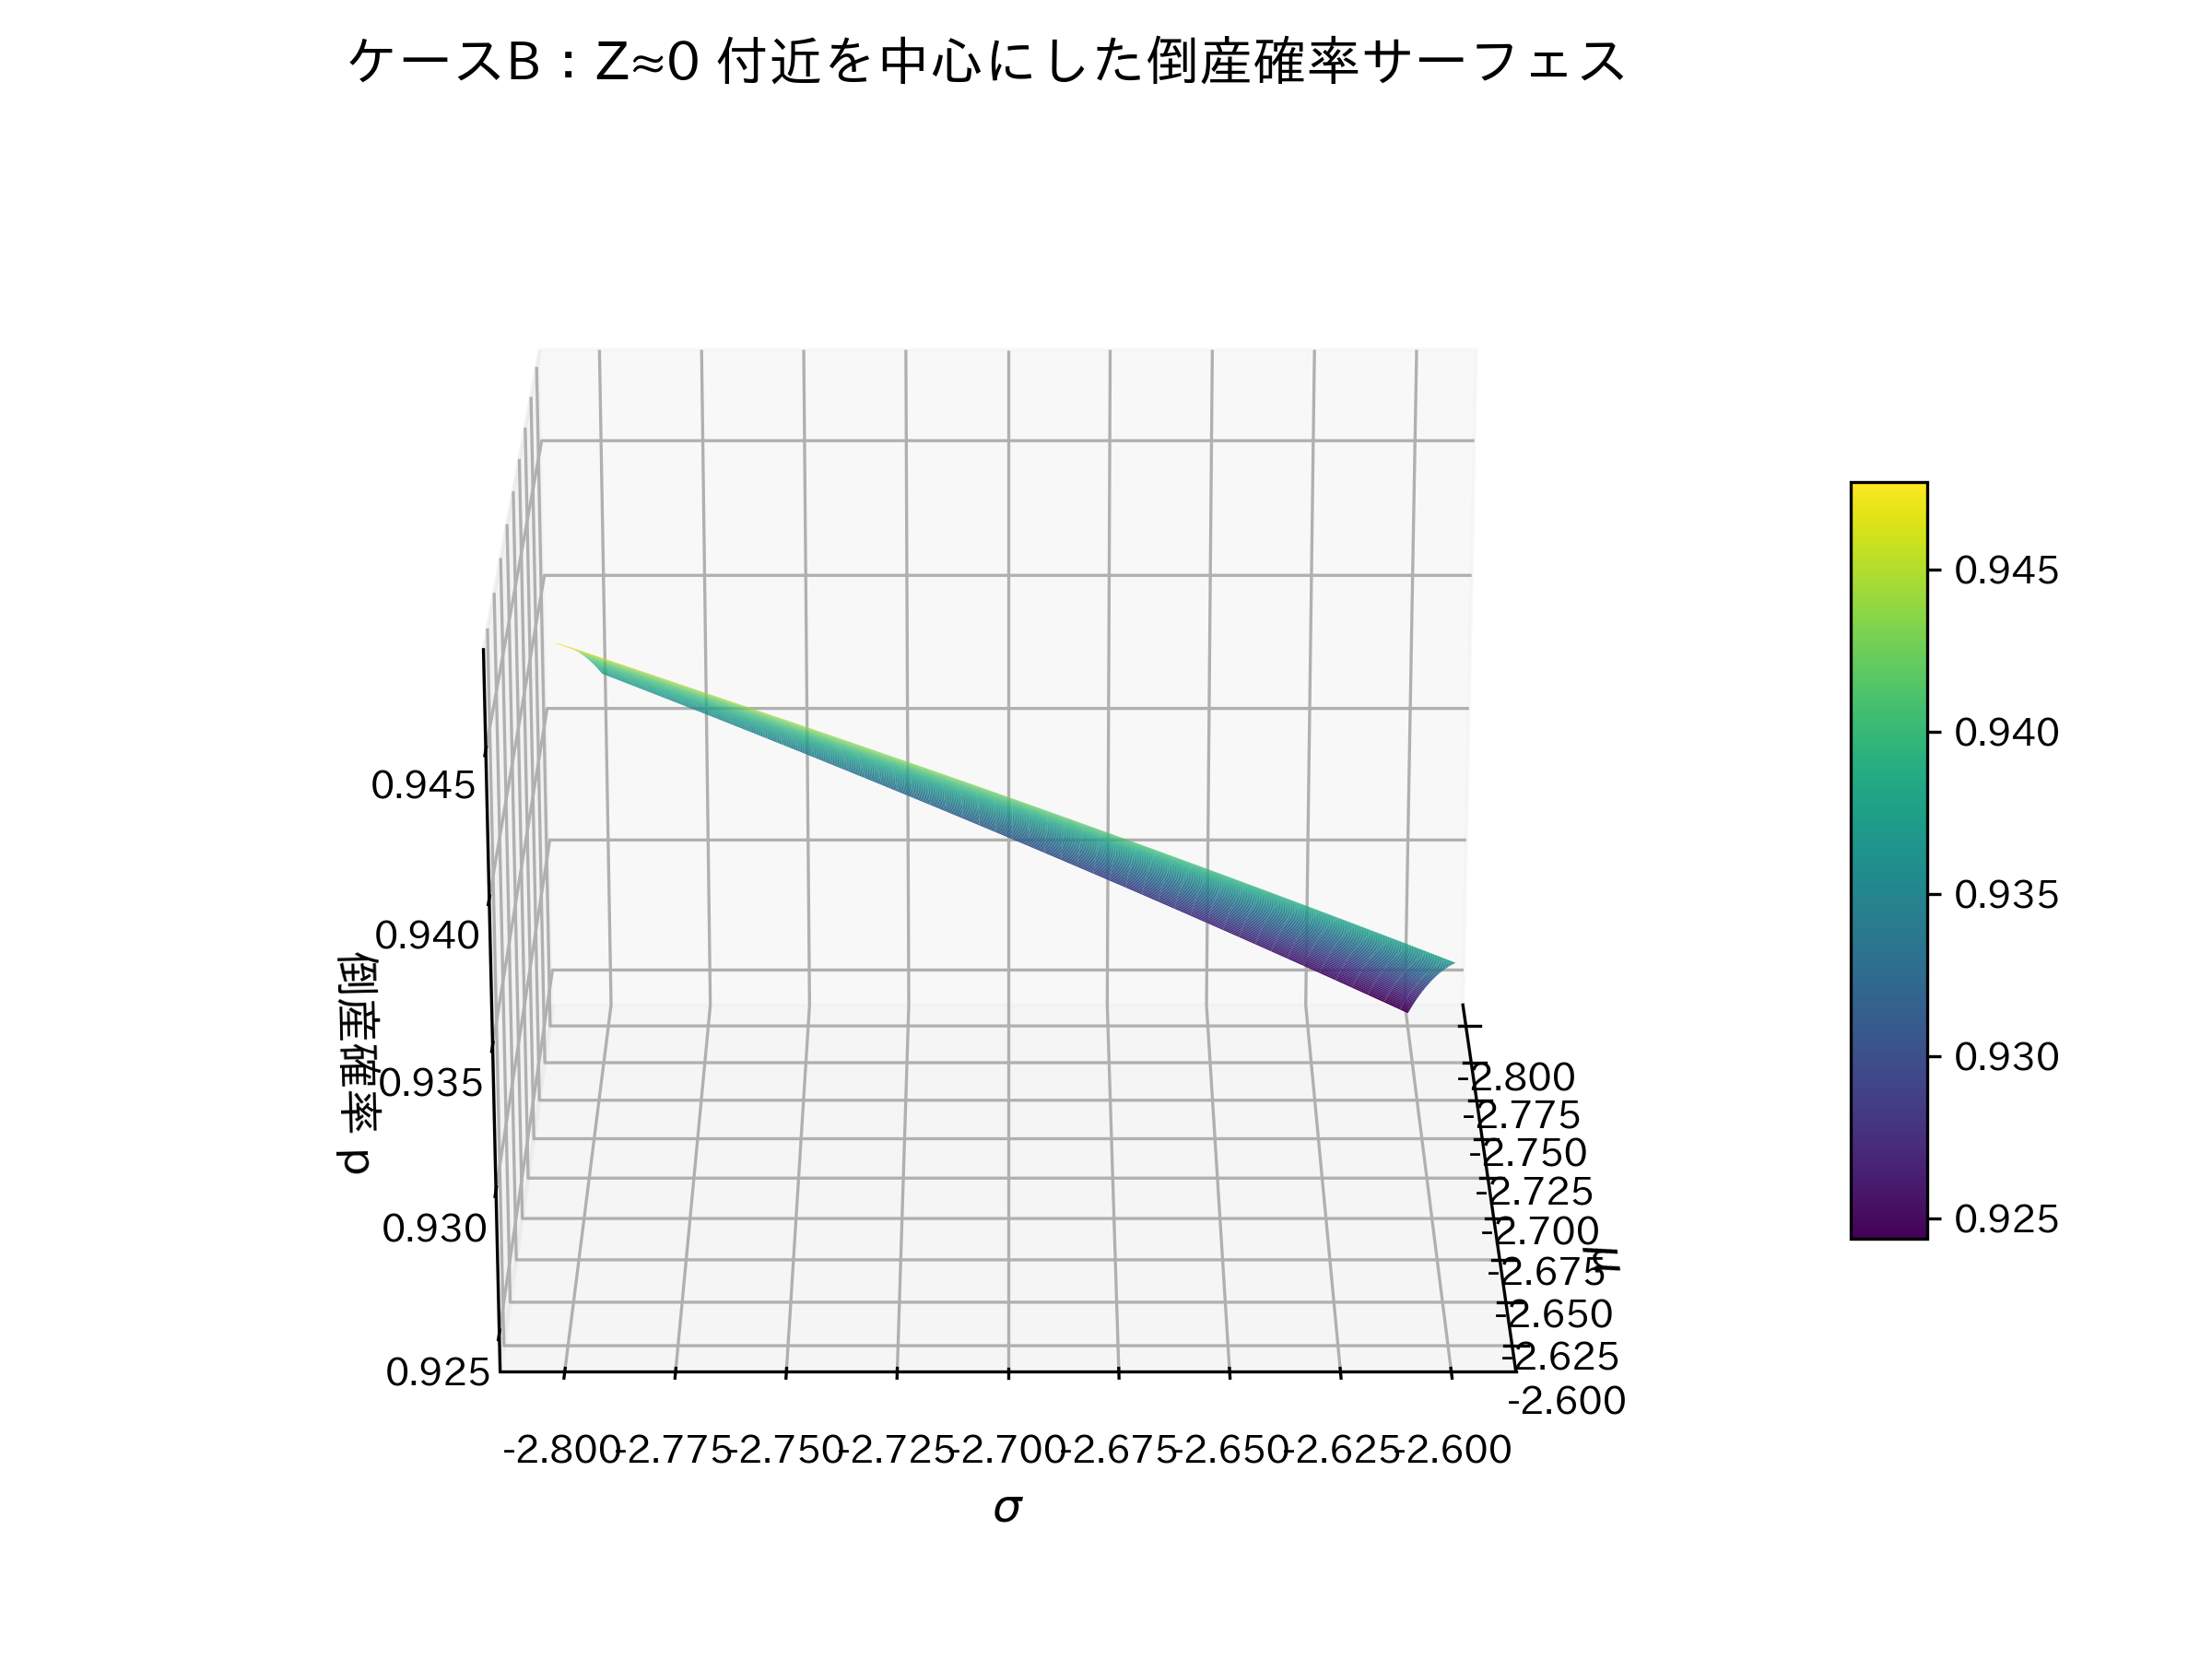
\includegraphics[width=0.75\linewidth]{figures/surface_caseB_centered.png}
    \caption{ケースBにおける倒産確率の3Dサーフェスプロット（Z≈0付近を中心）}
    \label{fig:surface_caseB_centered}
\end{figure}

ケースBでは，$S=3$ の強い支援能力により，
倒産確率の地形全体が大きく右方へシフトする。
Z≈0 を中心に描くことで，
支援能力が倒産境界線をどれほど押し下げるかが明確に可視化される。


% ---------- ケースC ----------
\subsubsection*{ケースC：$D=0.8,\ S=0$（独立系・負債過多）}

\begin{figure}[H]
    \centering
    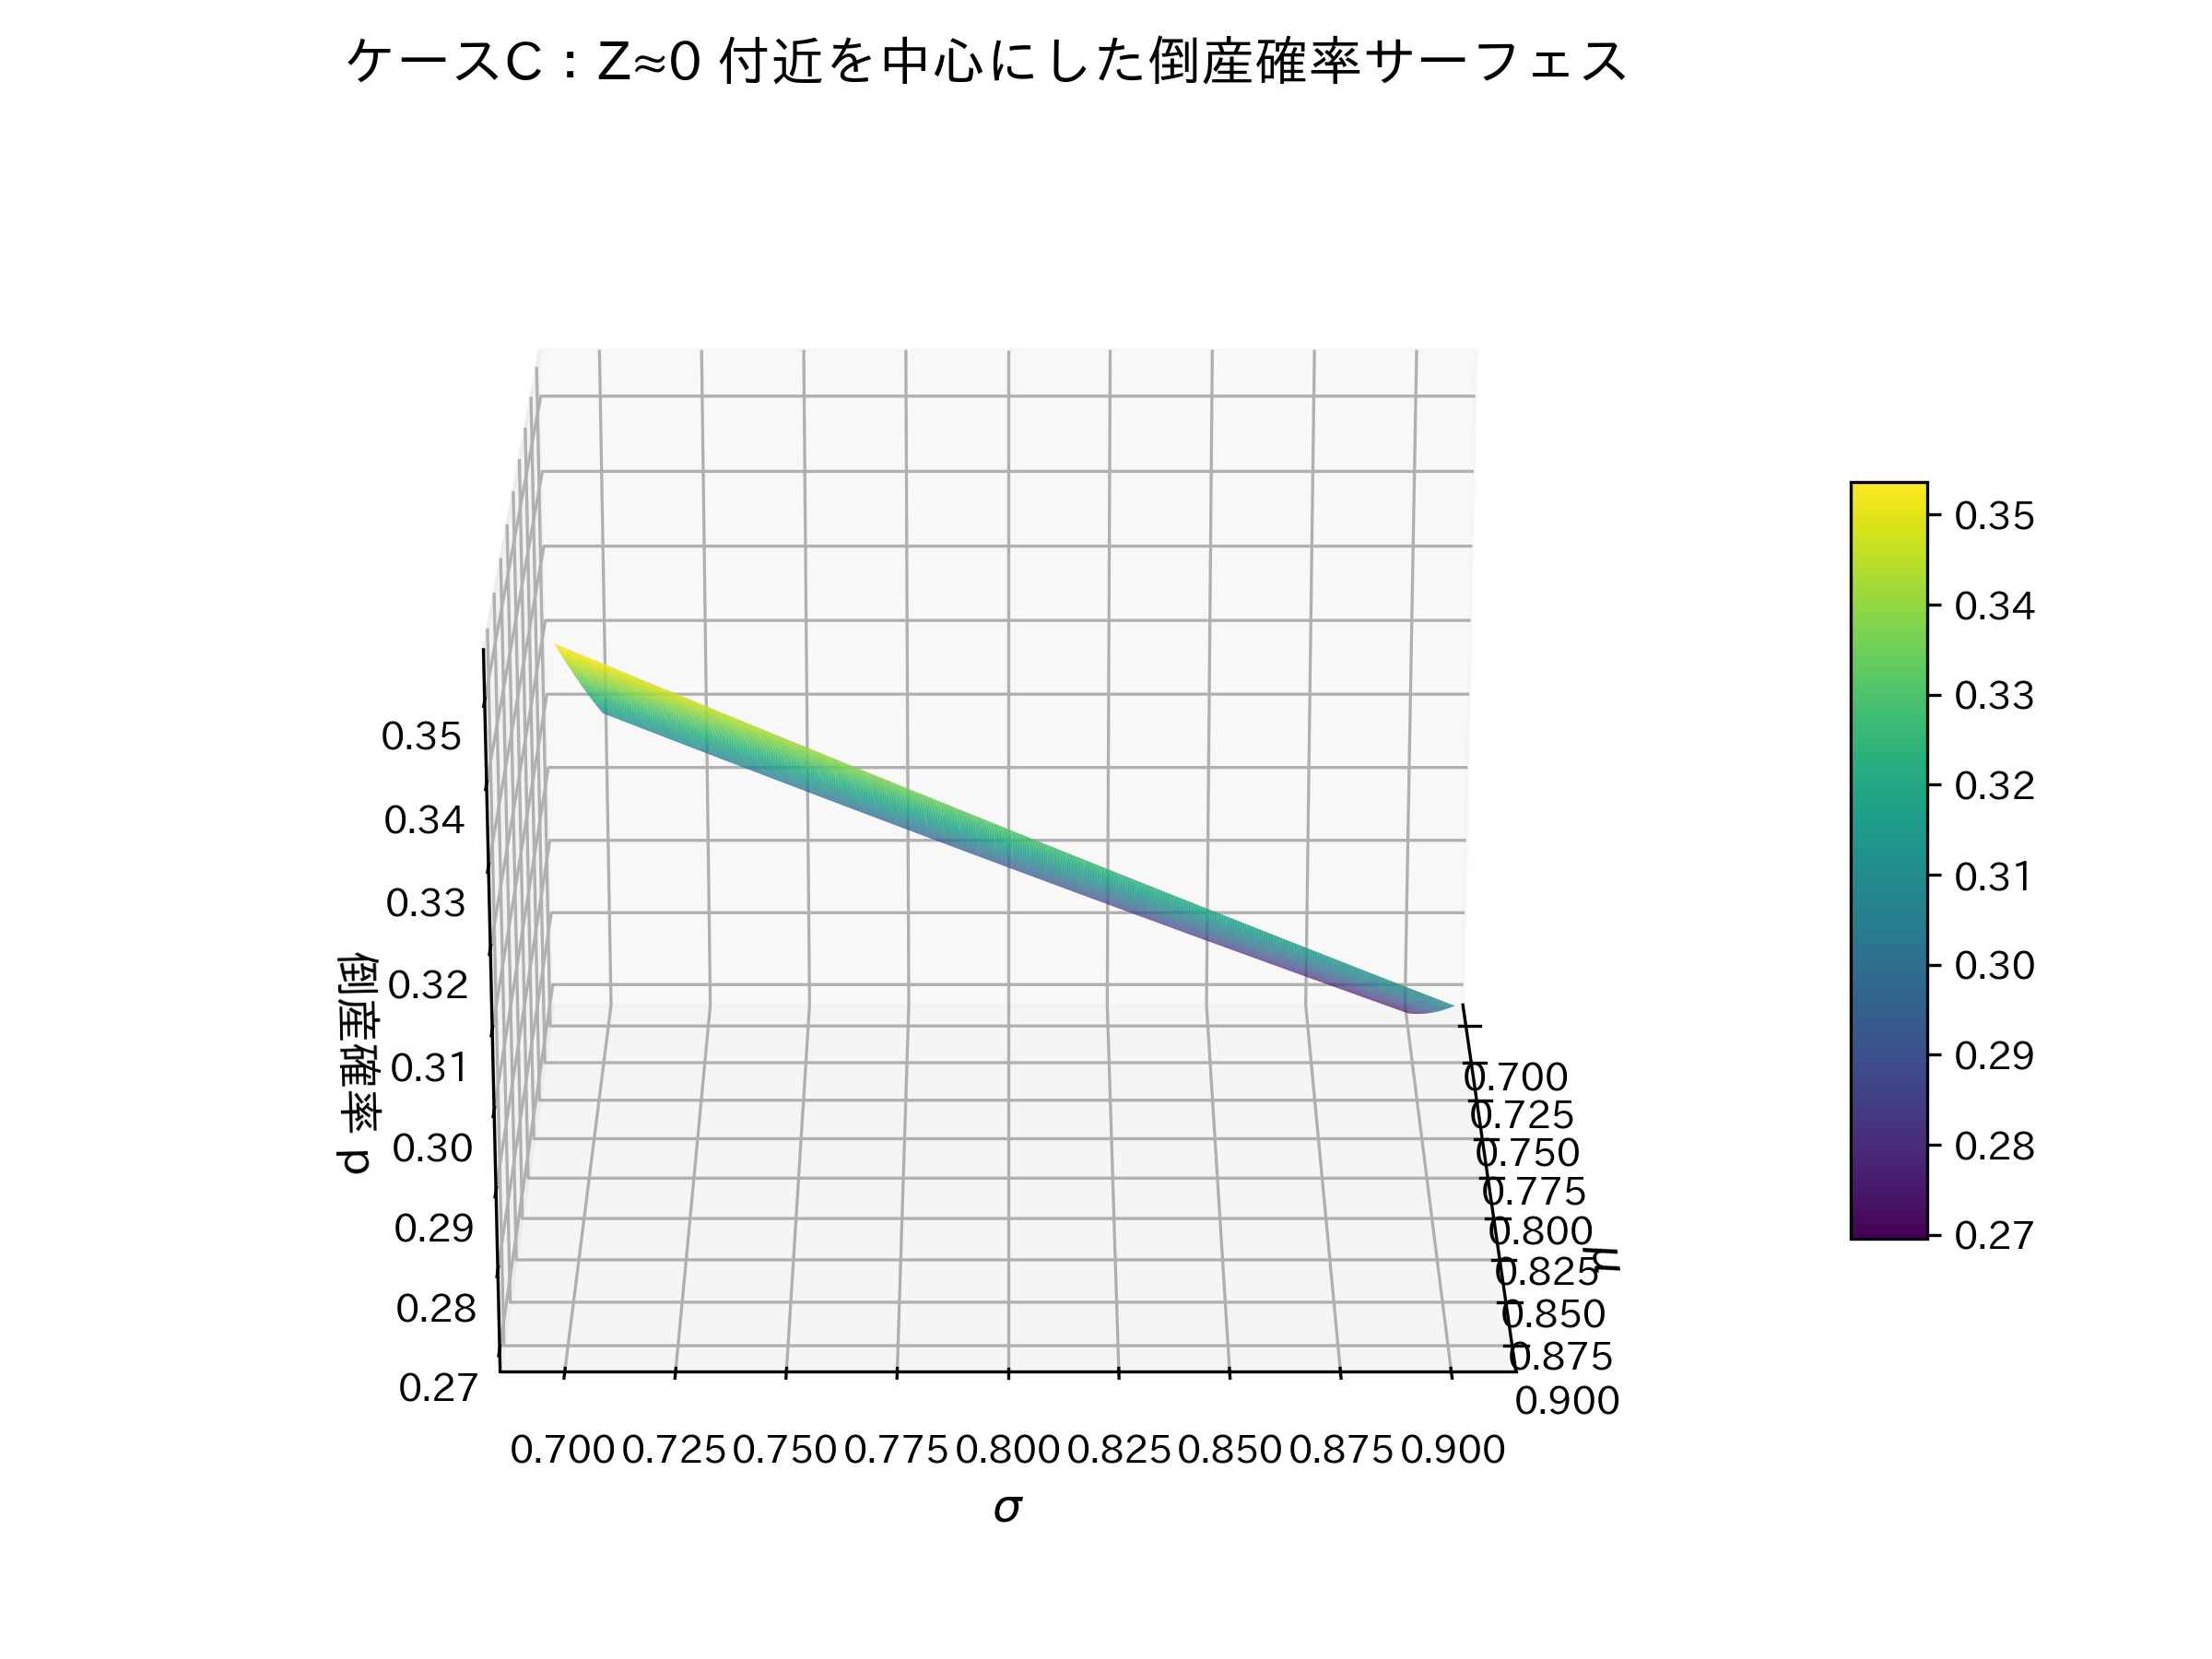
\includegraphics[width=0.75\linewidth]{figures/surface_caseC_centered.png}
    \caption{ケースCにおける倒産確率の3Dサーフェスプロット（Z≈0付近を中心）}
    \label{fig:surface_caseC_centered}
\end{figure}

ケースCでは，負債比率が高いため，
倒産確率の基準水準が大きく左方に位置し，倒産しやすい構造となる。
Z≈0 を中心に描くことで，
$\sigma$ の上昇に対する反応が極めて急峻であることが強調され，
高ボラティリティ環境での脆弱性が顕著に示される。


% ---------- ケースD ----------
\subsubsection*{ケースD：$D=0.8,\ S=3$（大手系・負債過多）}

\begin{figure}[H]
    \centering
    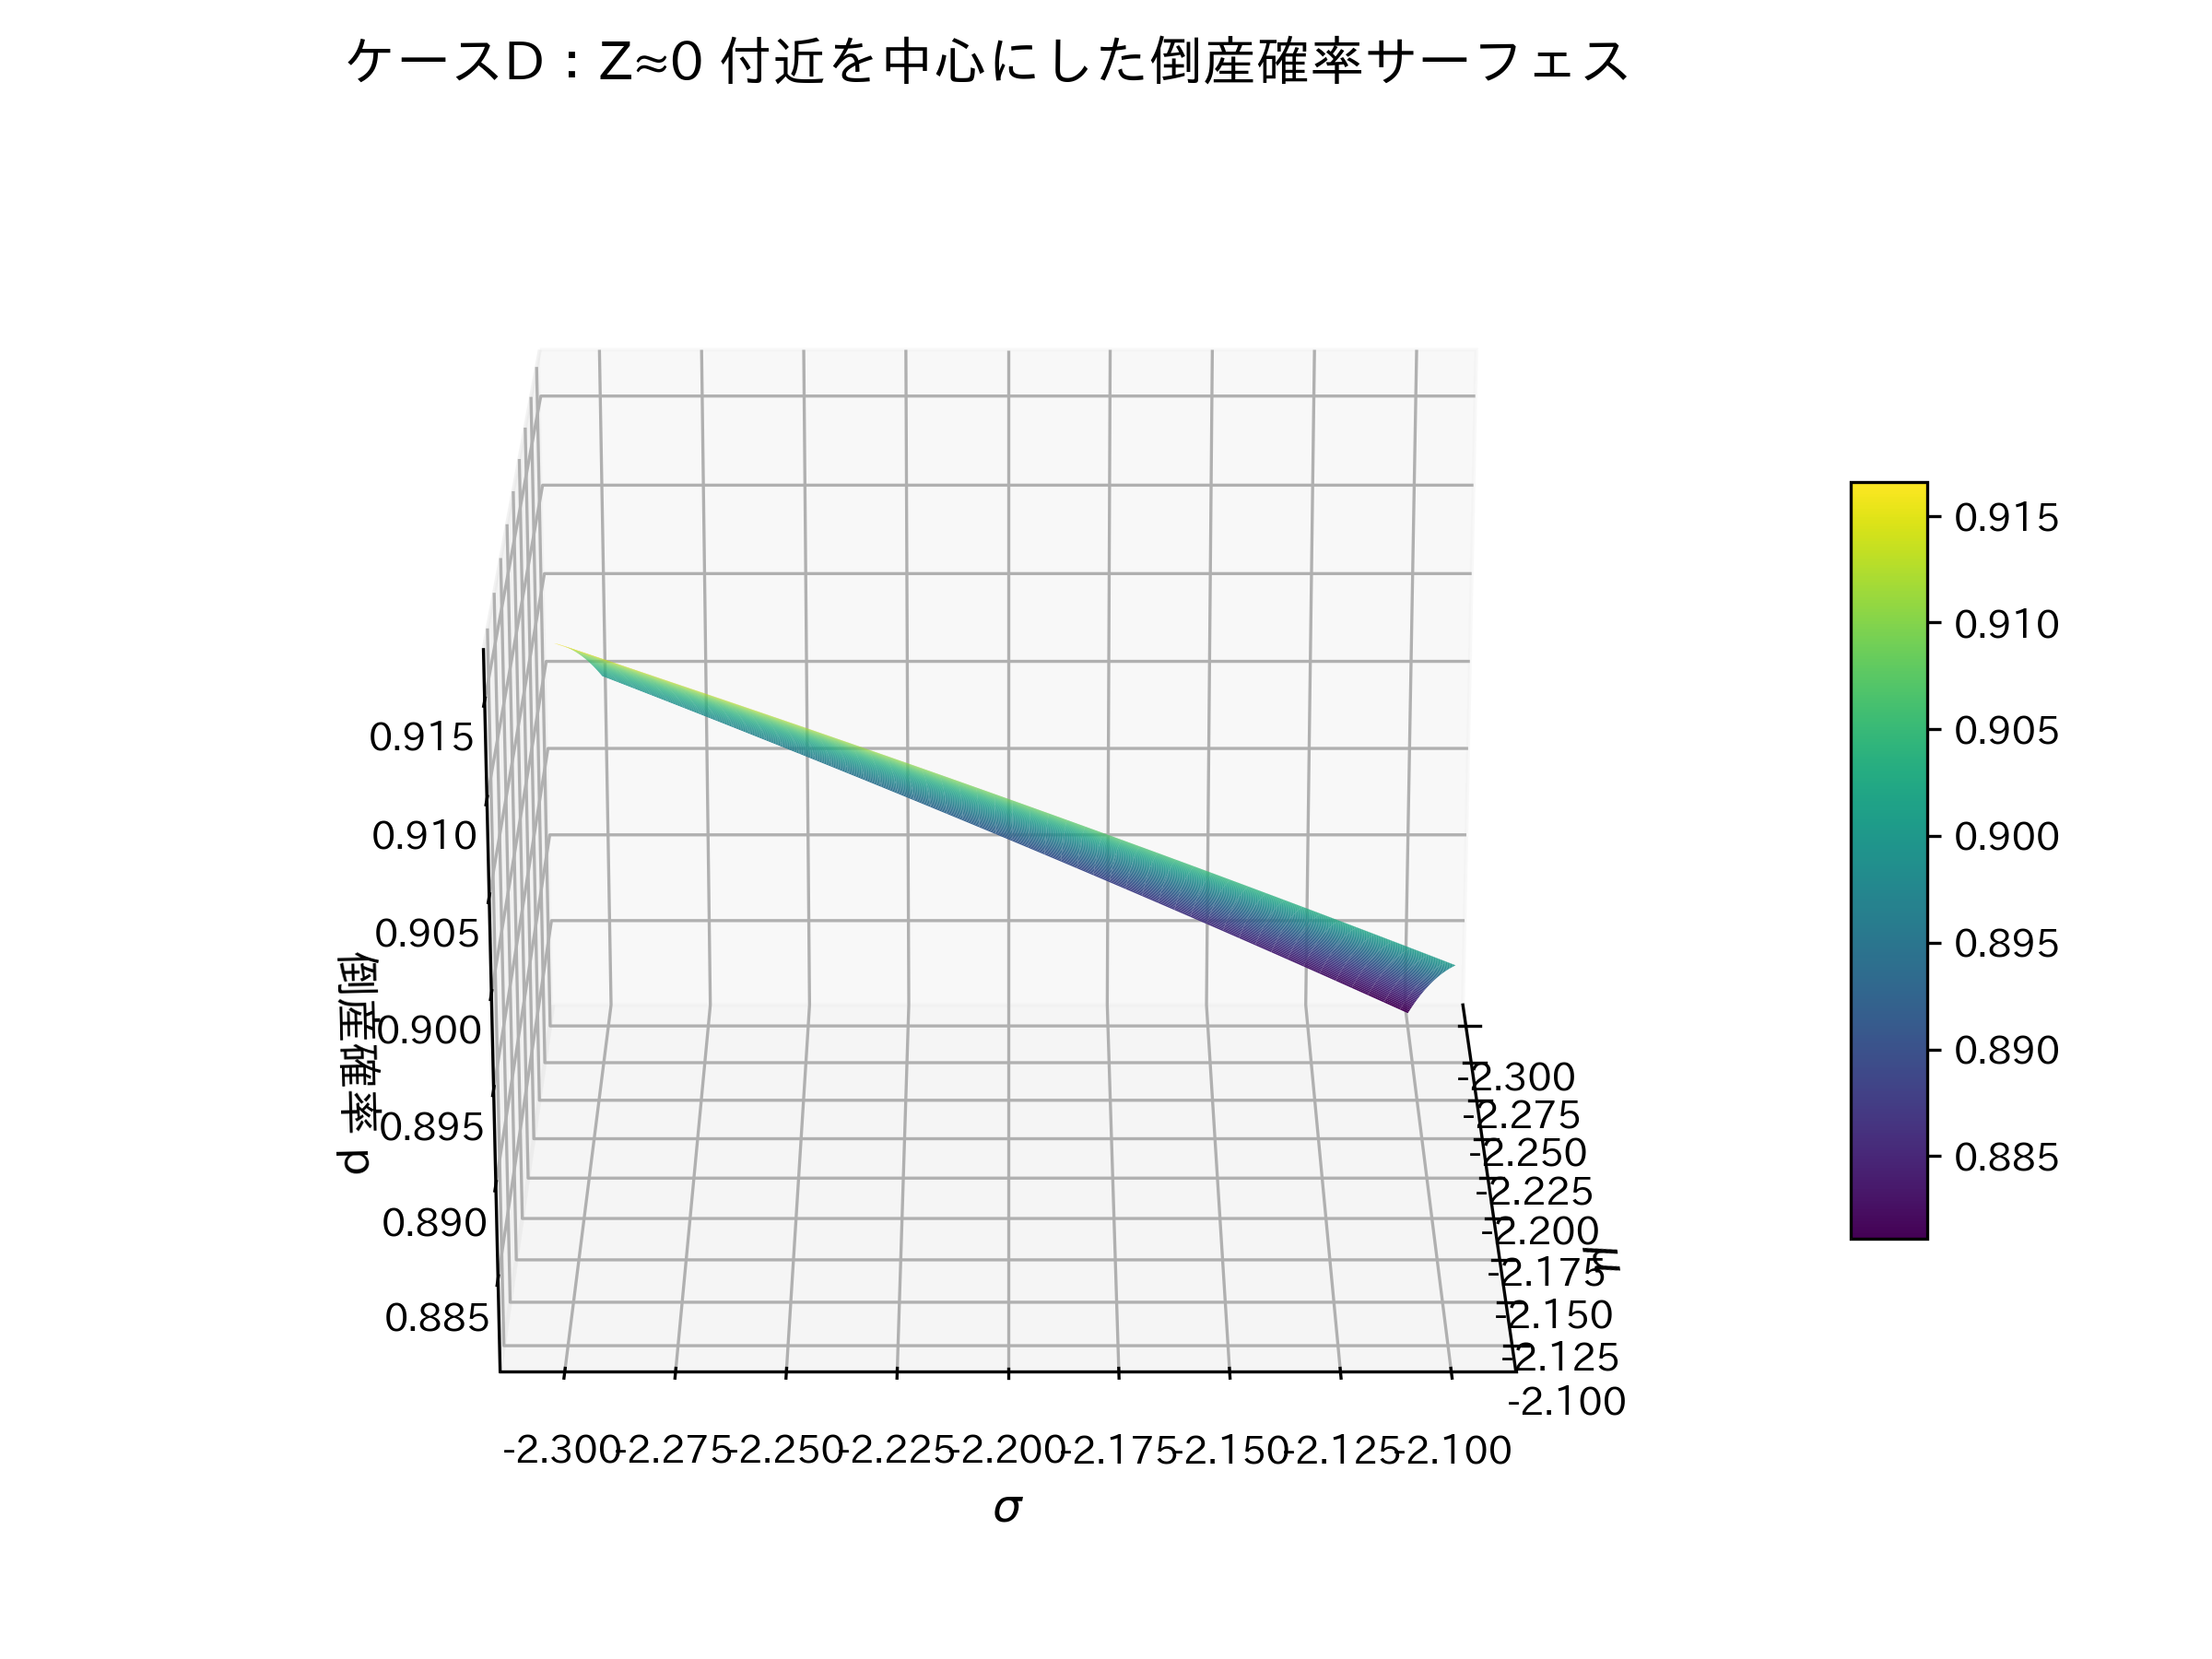
\includegraphics[width=0.75\linewidth]{figures/surface_caseD_centered.png}
    \caption{ケースDにおける倒産確率の3Dサーフェスプロット（Z≈0付近を中心）}
    \label{fig:surface_caseD_centered}
\end{figure}

ケースDでは，負債比率は高いものの，
強い支援能力により倒産確率の地形が右方へ押し戻される。
Z≈0 を中心に描くことで，
「高負債 × 強支援」という構造が倒産境界線の位置にどのように反映されるかが明確となる。
ただし $\sigma$ の影響は依然として大きく，
高ボラティリティ環境でのリスクは残存する。


% ---------- ケースE ----------
\subsubsection*{ケースE：$D=0.5,\ S=1$（地域新電力）}

\begin{figure}[H]
    \centering
    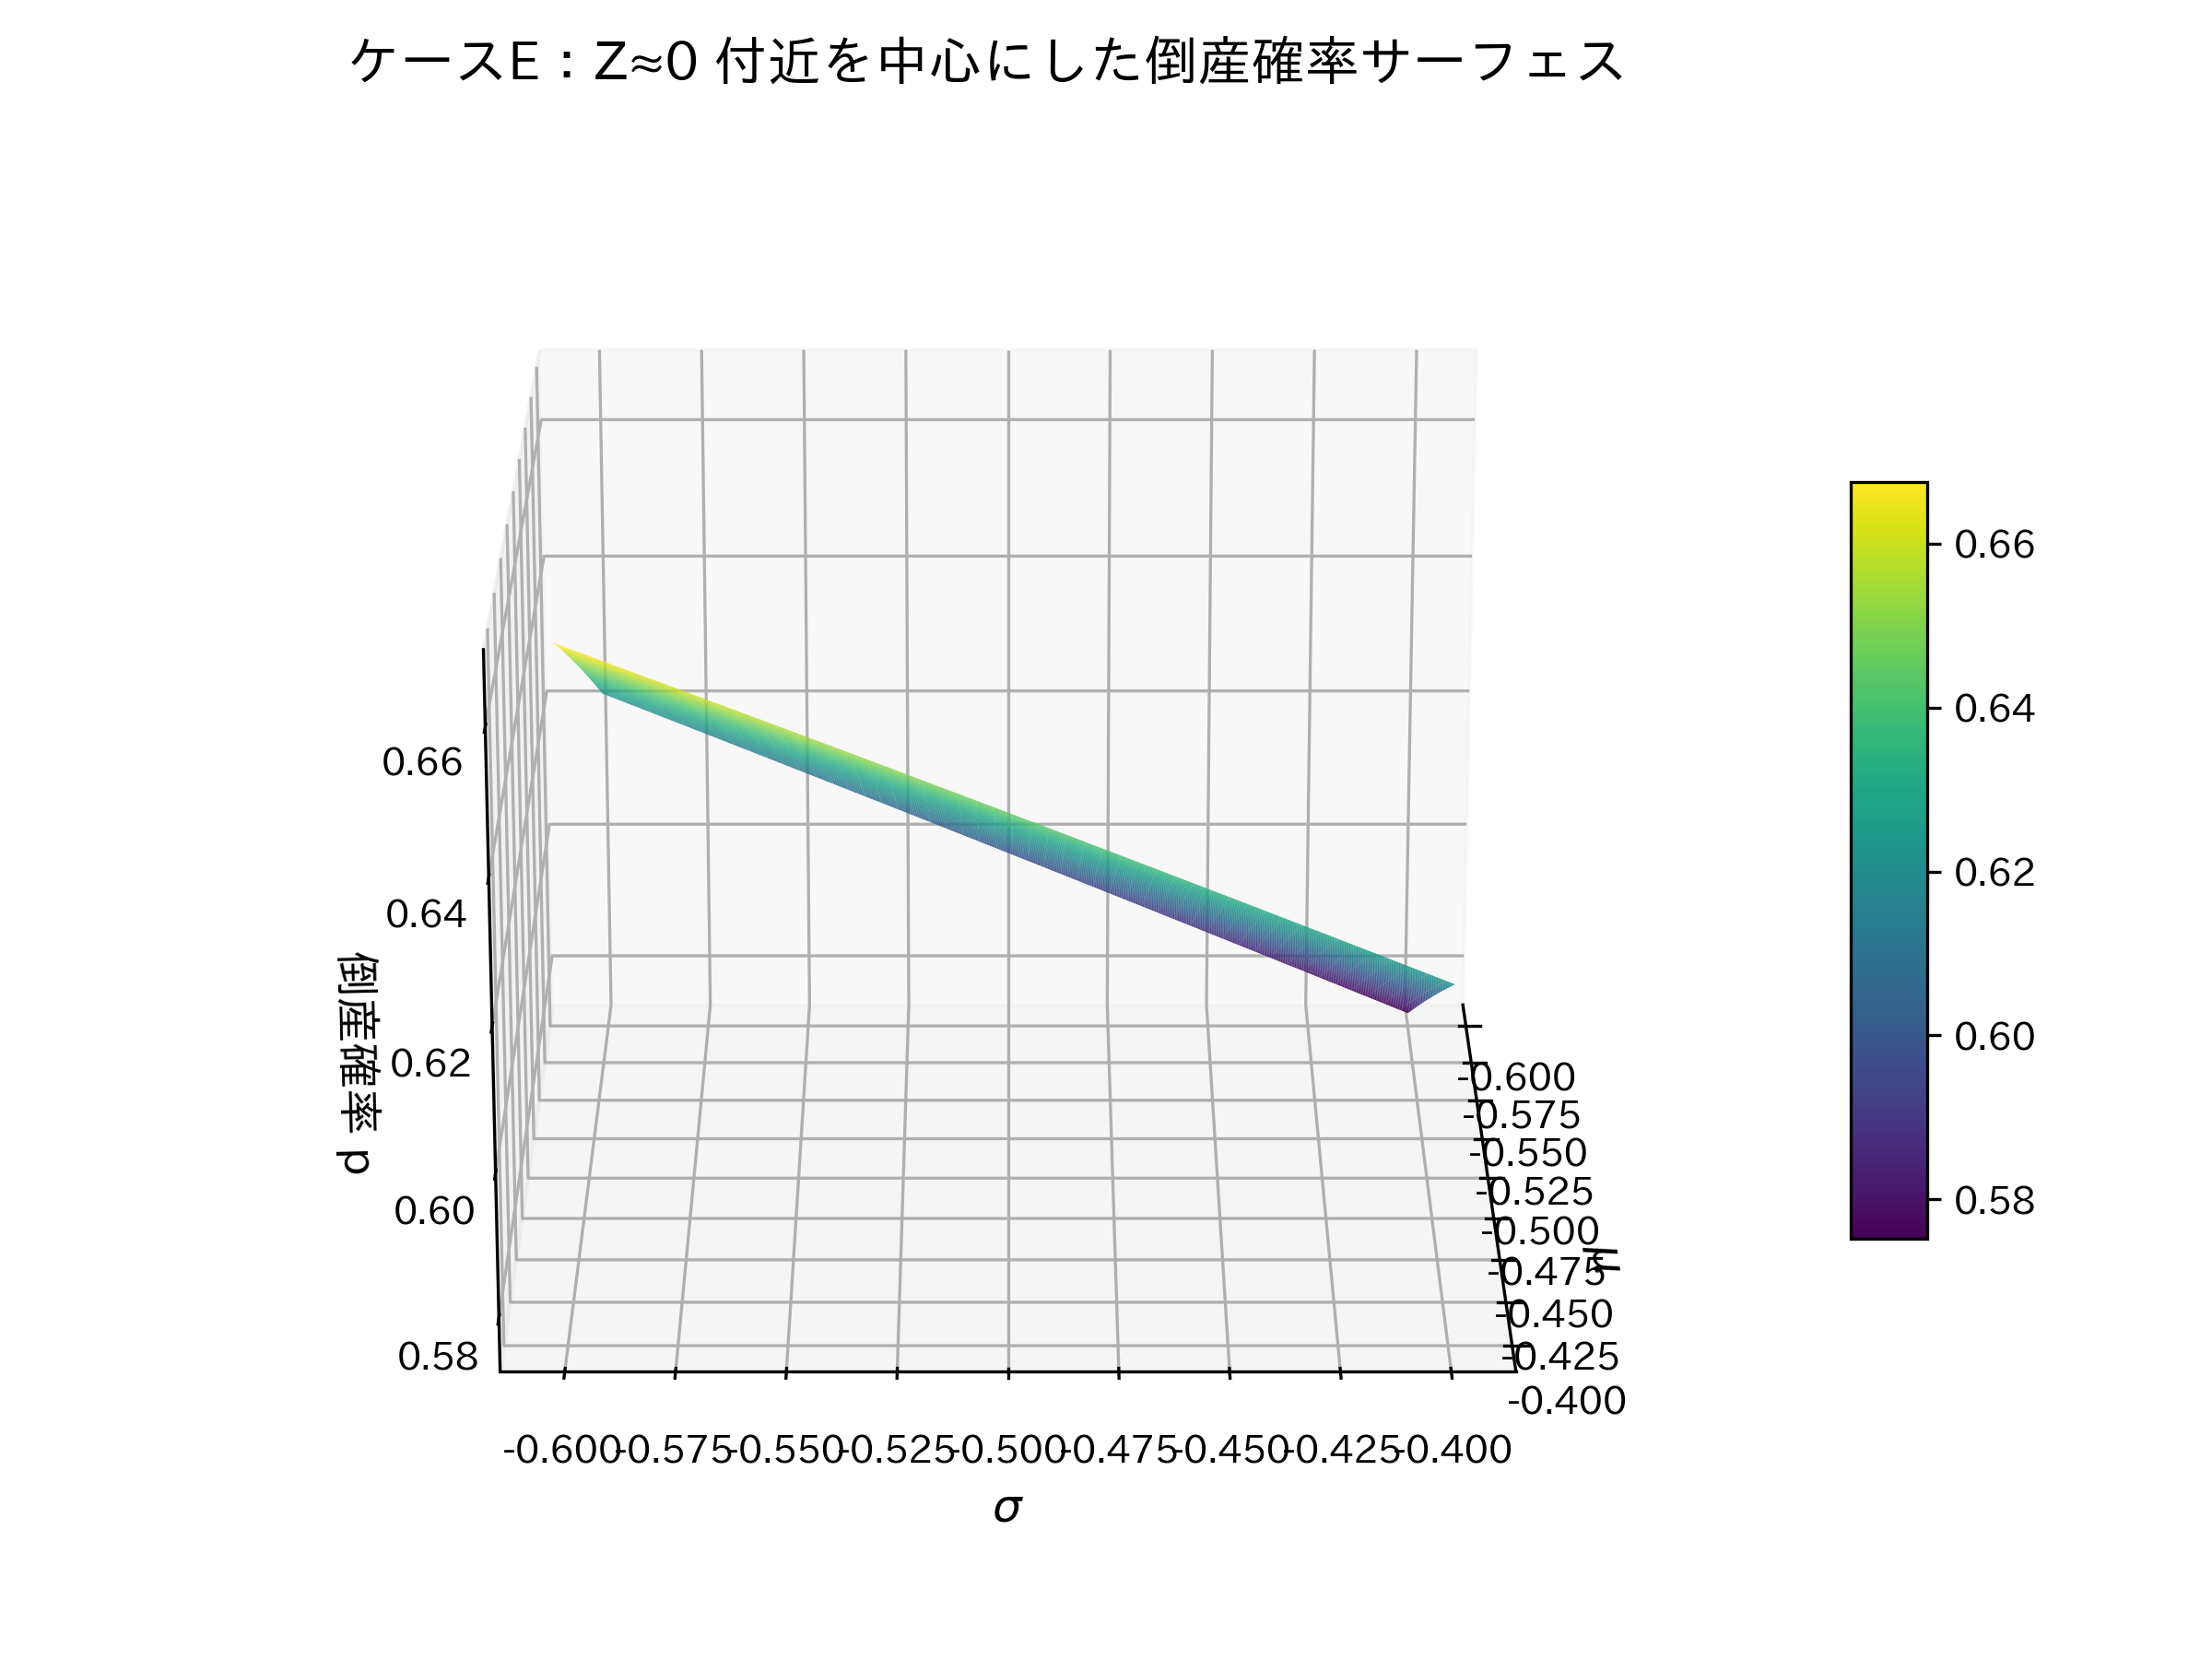
\includegraphics[width=0.75\linewidth]{figures/surface_caseE_centered.png}
    \caption{ケースEにおける倒産確率の3Dサーフェスプロット（Z≈0付近を中心）}
    \label{fig:surface_caseE_centered}
\end{figure}

ケースEは中程度の負債比率と限定的な支援能力を持つ典型的な地域新電力であり，
倒産確率の地形は中間的な位置にある。
Z≈0 を中心に描くことで，
$\mu$ の改善効果が比較的強く，収益性の改善がリスク低下に直結する構造が明確に示される。


% ---------- ケースF ----------
\subsubsection*{ケースF：$D=0.5,\ S=2$（商社系）}

\begin{figure}[H]
    \centering
    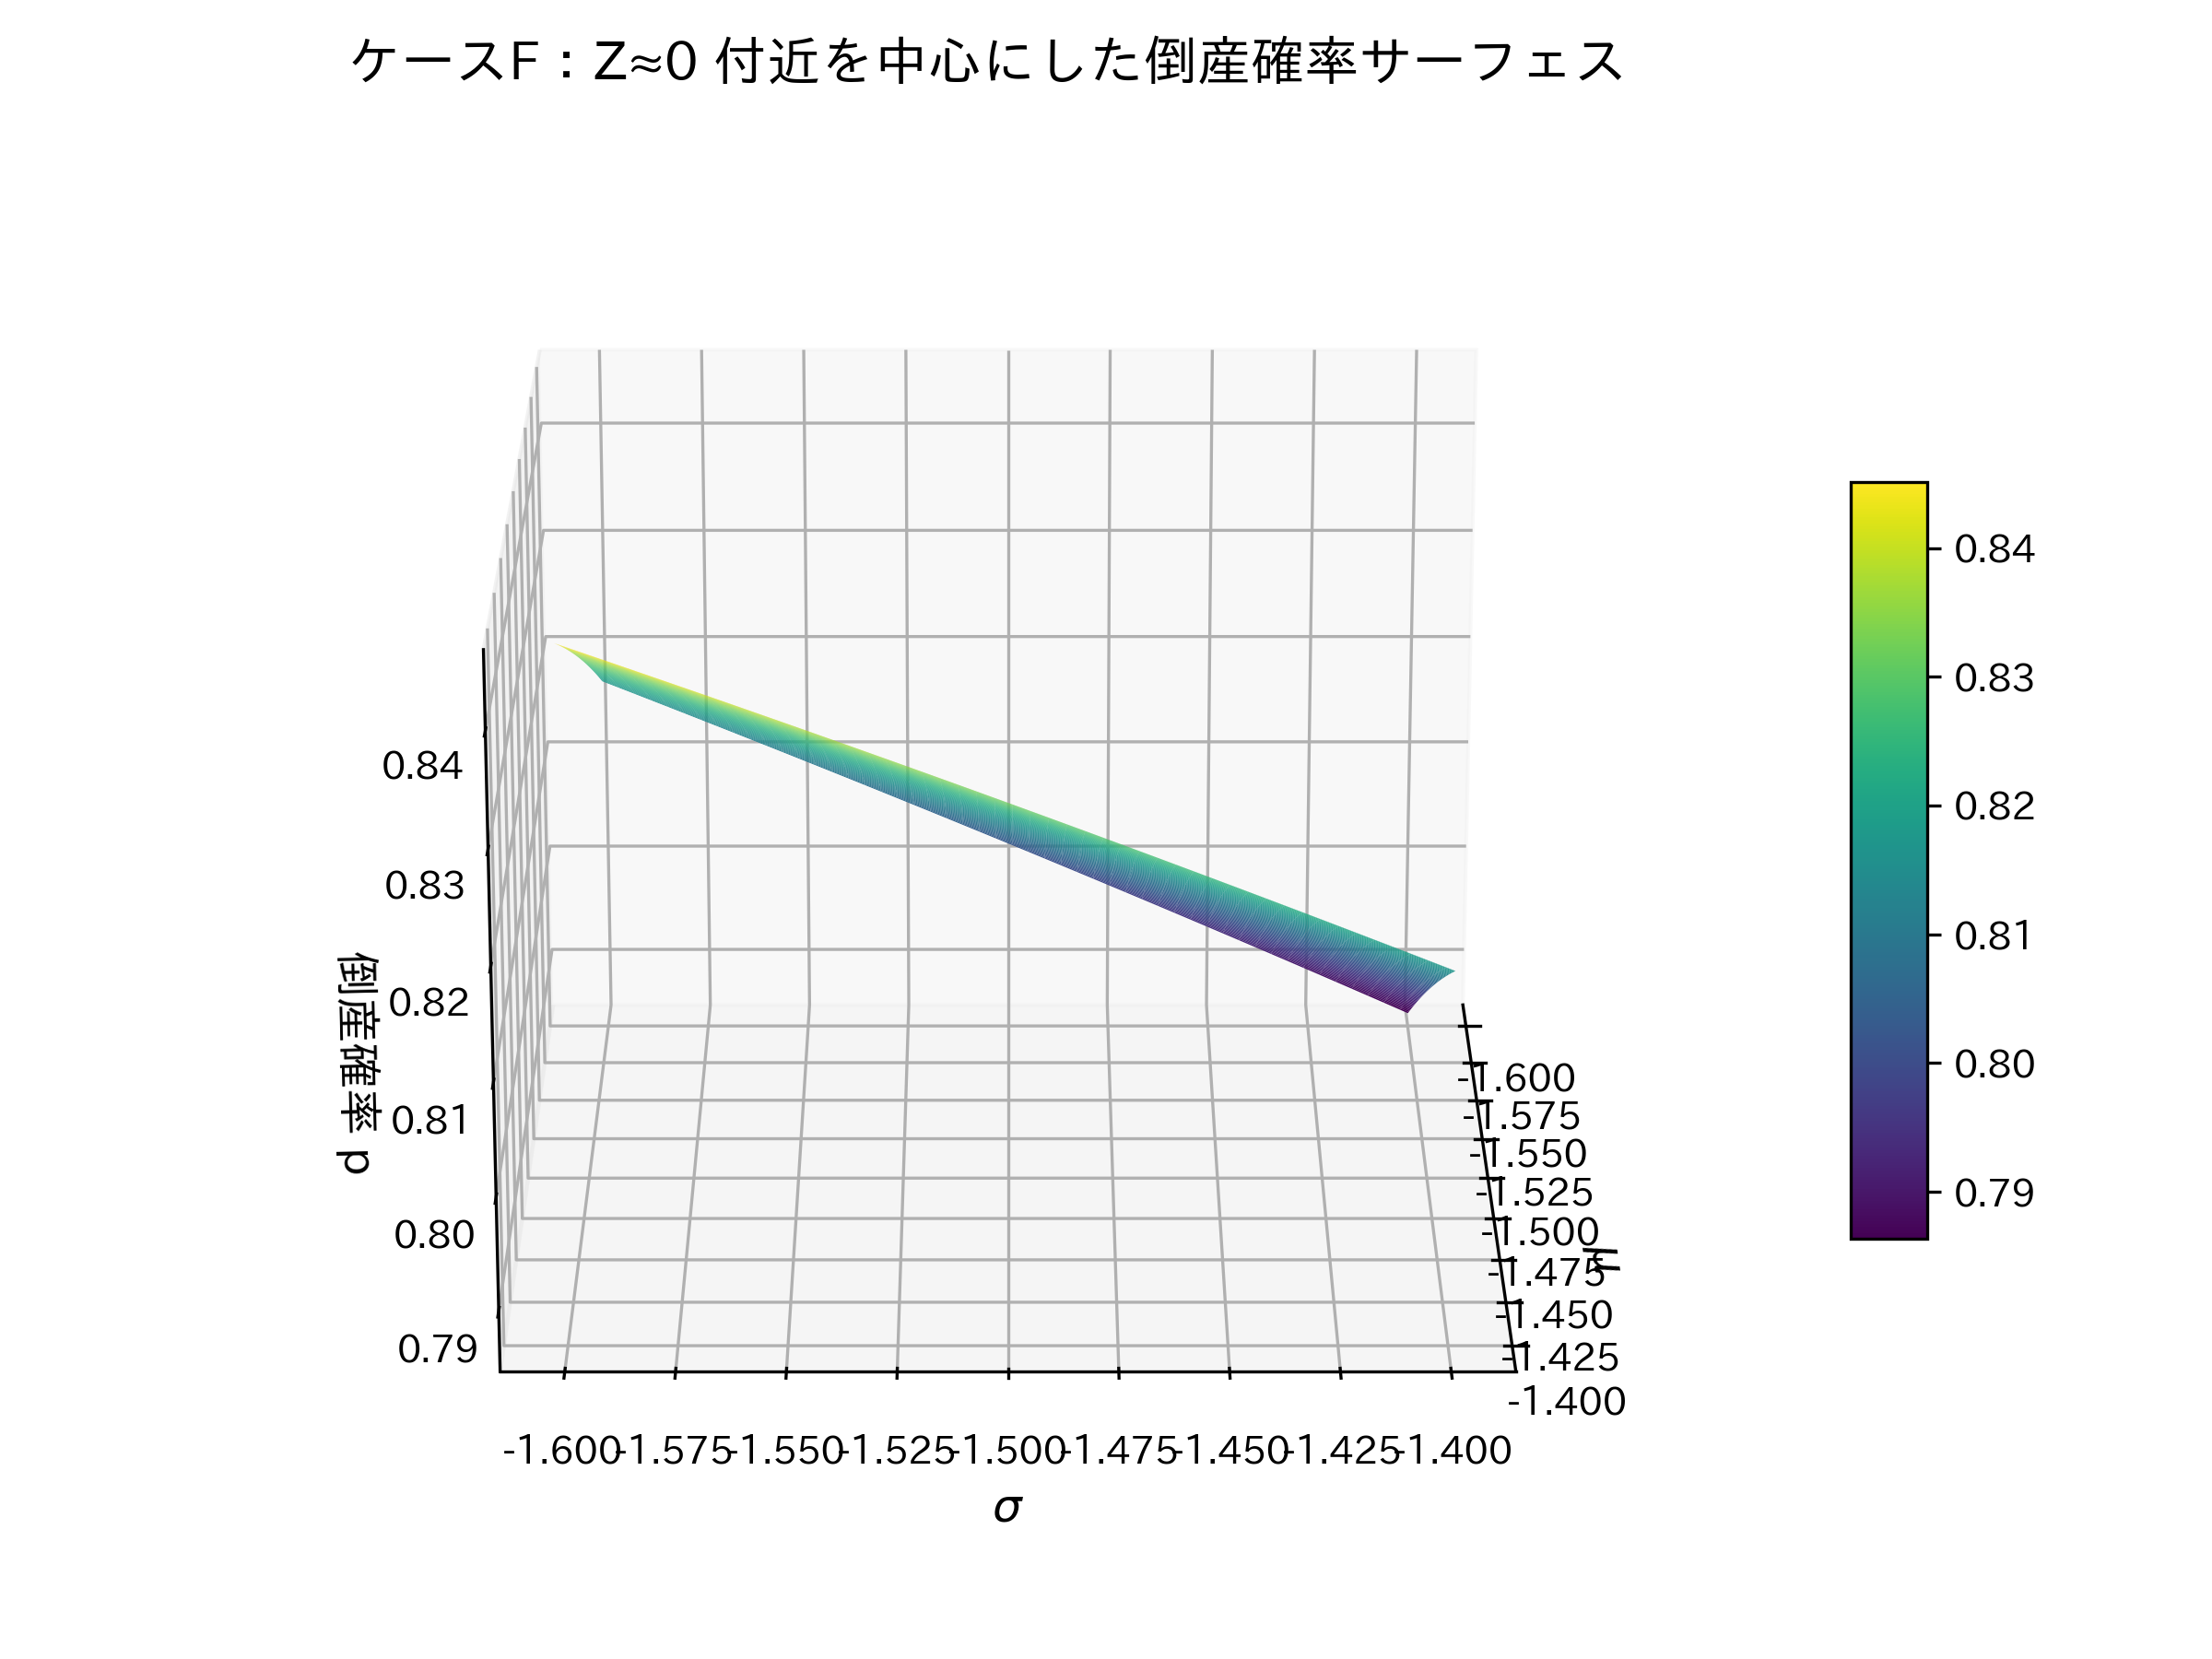
\includegraphics[width=0.75\linewidth]{figures/surface_caseF_centered.png}
    \caption{ケースFにおける倒産確率の3Dサーフェスプロット（Z≈0付近を中心）}
    \label{fig:surface_caseF_centered}
\end{figure}

ケースFでは，商社系の強い支援能力により，
倒産確率の地形はケースEより右方に位置する。
Z≈0 を中心に描くことで，
支援能力が倒産境界線を大きく押し下げる効果が視覚的に確認でき，
外生ショックに対する耐性が向上していることが示される。


\subsection*{大企業と地方電力の倒産リスク格差と，小規模企業が生き残る条件}

本節では，倒産確率の差分


\[
\Delta p = p_{\mathrm{B}} - p_{\mathrm{C}}
\]


を算出し，大企業（ケースB：$D=0.3,\ S=3$）と，
地方電力で資本支援のない企業（ケースC：$D=0.8,\ S=0$）の
倒産リスク格差を可視化する。
図\ref{fig:surface_diff_B_minus_C} に示すとおり，
$\Delta p$ は全域で正となり，
大企業の倒産確率が地方電力より一貫して低いことが確認できる。

\begin{figure}[H]
    \centering
    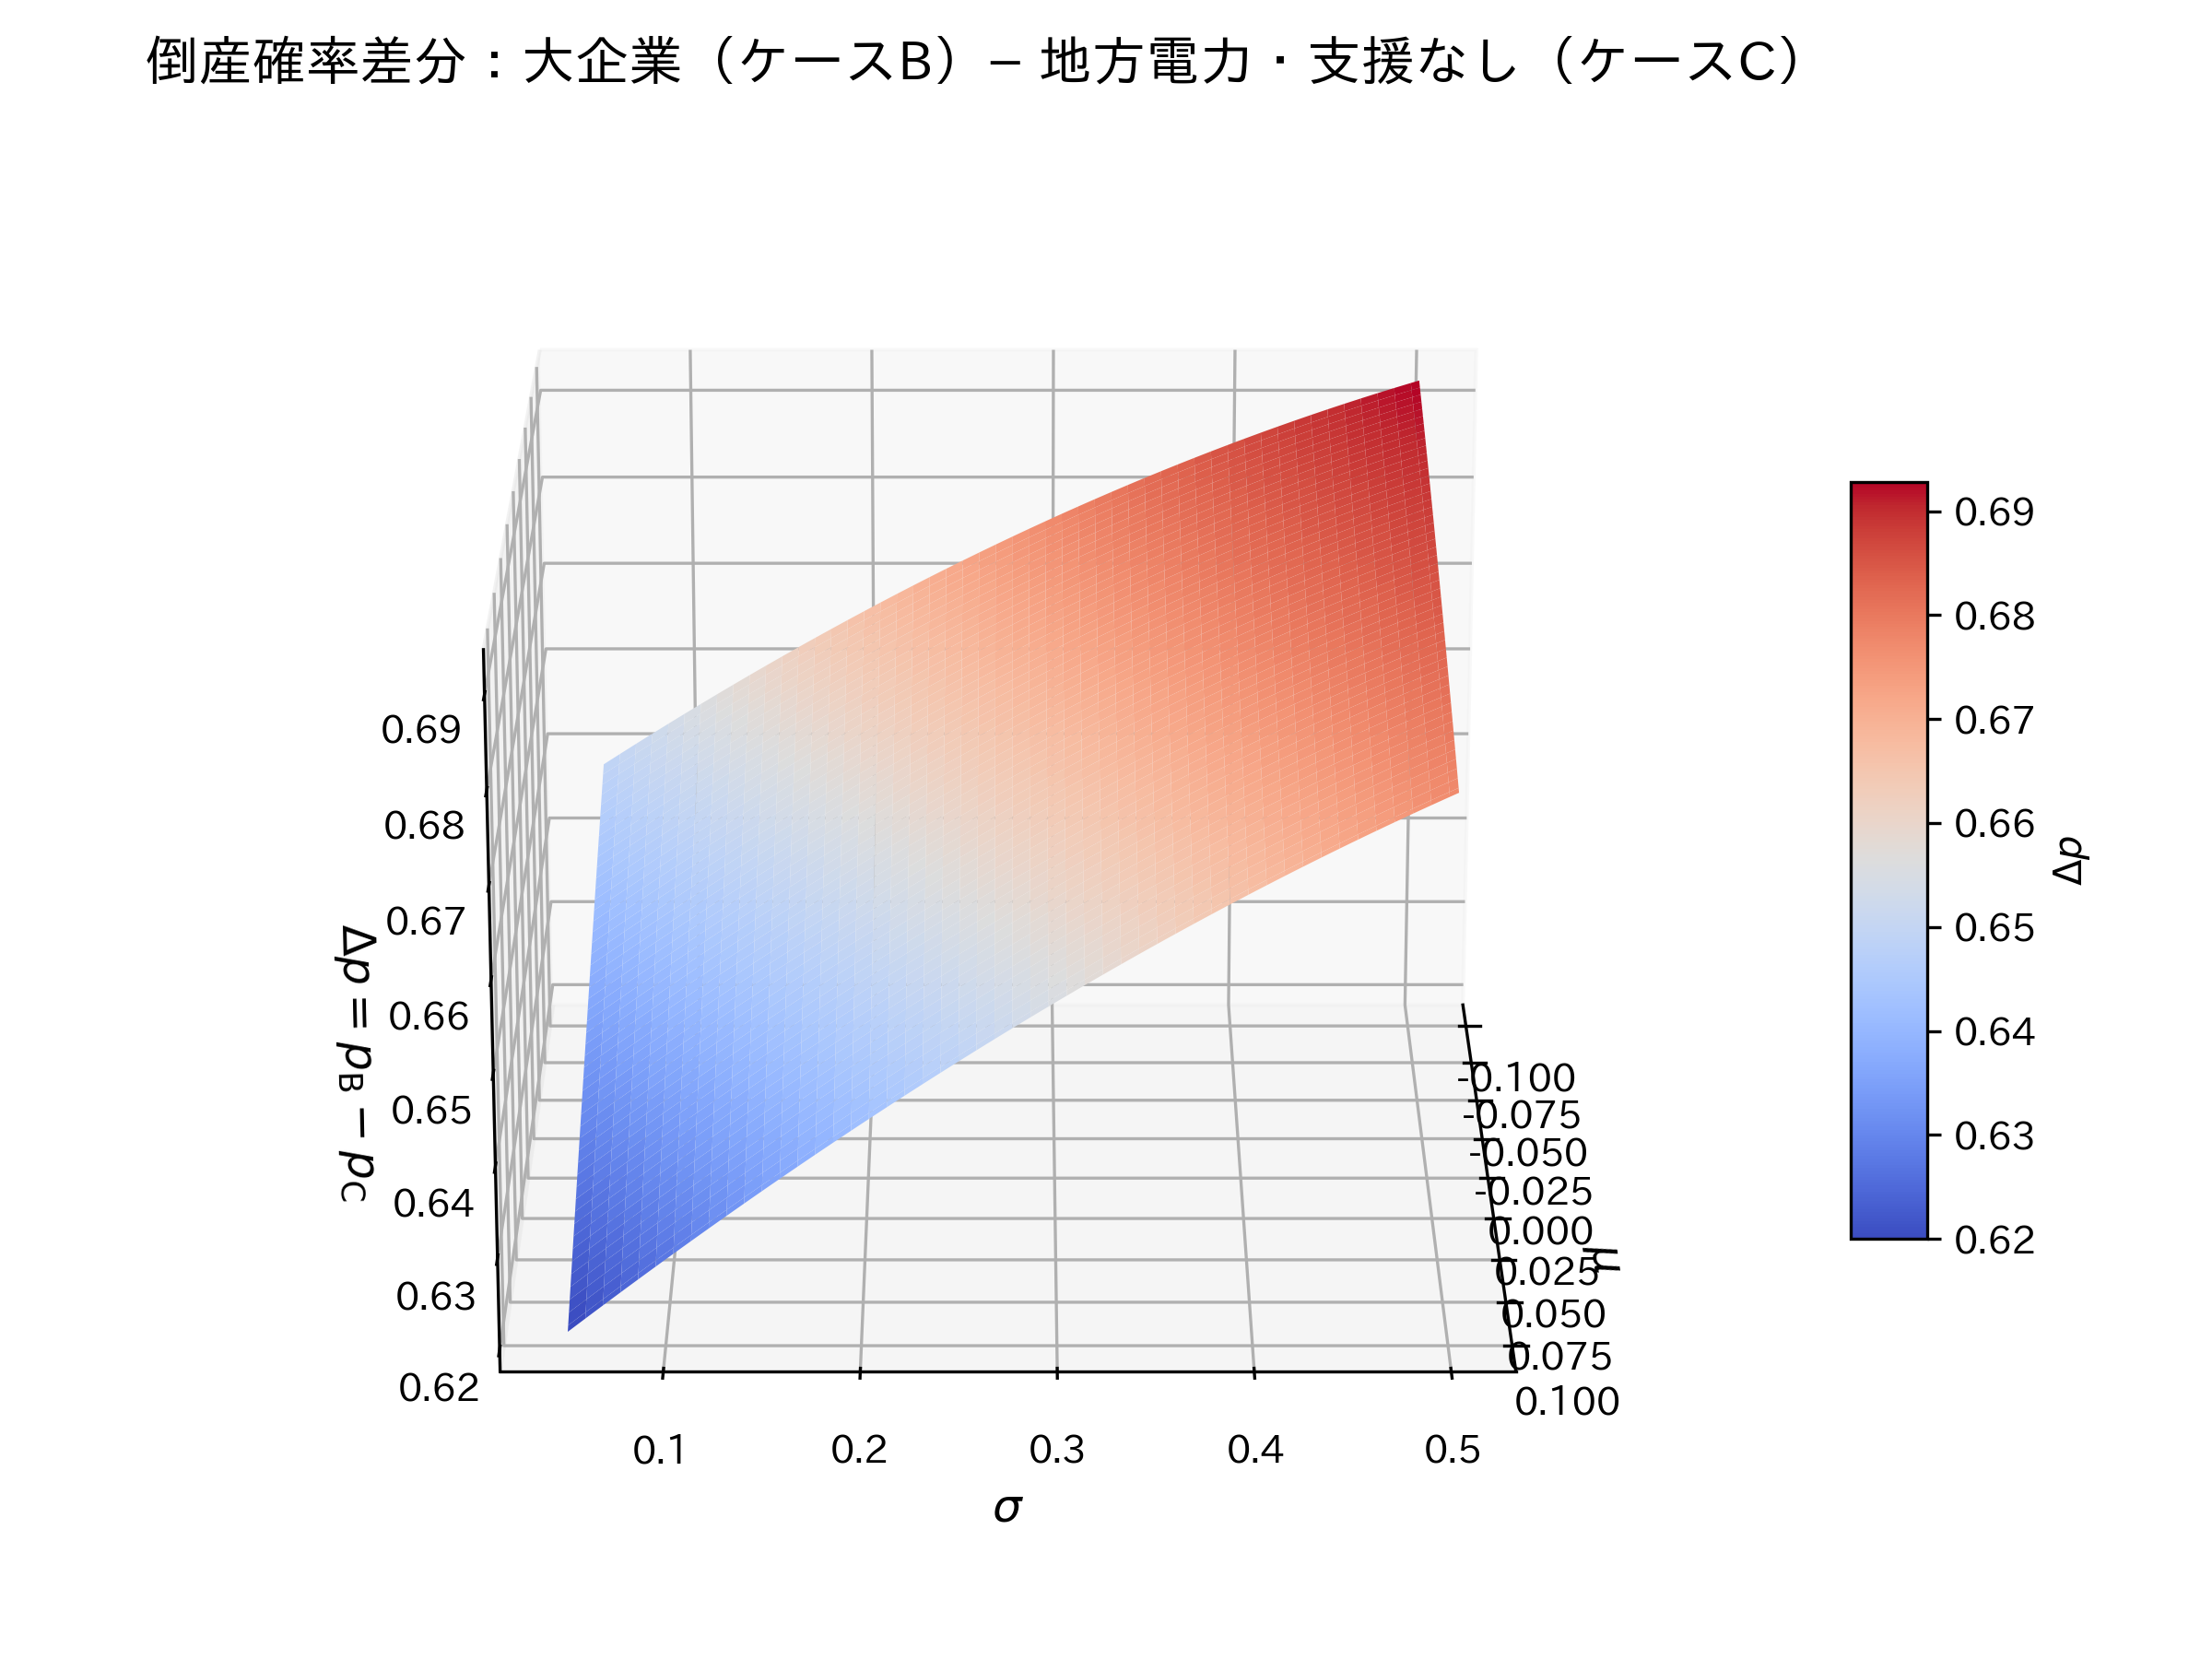
\includegraphics[width=0.75\linewidth]{figures/surface_diff_B_minus_C.png}
    \caption{倒産確率の差分サーフェス：大企業（ケースB）$-$ 地方電力・支援なし（ケースC）}
    \label{fig:surface_diff_B_minus_C}
\end{figure}

図\ref{fig:surface_diff_B_minus_C} の形状は，
倒産リスク格差が $\mu$（収益性）および $\sigma$（市場ショック）の関数として
どのように拡大・縮小するかを示している。
特に以下の3点が重要である。

\begin{enumerate}
    \item \textbf{市場ショックが大きいほど格差が拡大する}  
    $\sigma$ が大きい領域では $\Delta p$ が急速に増加しており，
    市場変動に対する脆弱性が地方電力に集中していることがわかる。
    大企業は支援能力 $S=3$ によりショックを吸収できる一方，
    地方電力は $\sigma$ の上昇に対して倒産確率が急激に上昇する。

    \item \textbf{収益性が低いほど格差が最大化する}  
    $\mu$ が負の領域では $\Delta p$ が最も大きく，
    収益性の低下が地方電力の倒産確率を大幅に押し上げる。
    大企業は $\mu$ が低くても支援能力により倒産確率が抑制されるため，
    両者の差が顕著に現れる。

    \item \textbf{支援能力（$S$）の有無が倒産確率を決定づける}  
    本モデルでは，負債比率 $D$ や収益性 $\mu$ 以上に，
    支援能力 $S$ が倒産確率に強く作用する。
    ケースBとケースCの差分が 0.6〜0.7 程度に達することは，
    支援能力の有無が企業存続に与える影響が極めて大きいことを示している。
\end{enumerate}

以上の結果は，「大企業が倒産しにくい」という自明な事実を確認するだけではなく，
\textbf{小規模企業であっても生き残るための条件が存在する}ことを
数理モデルにより明確に示している点に意義がある。
すなわち，

\begin{itemize}
    \item 収益性 $\mu$ を一定以上確保すること（価格戦略・コスト削減）
    \item 市場ショック $\sigma$ を低減すること（固定価格契約・ヘッジ）
    \item 支援能力 $S$ を部分的にでも確保すること（自治体・地銀・地域企業との連携）
    \item 負債比率 $D$ を抑制すること（過剰借入の回避）
\end{itemize}

が，小規模企業の倒産確率を大幅に低減させる「生存条件」として導かれる。

本章のシミュレーションは，
大企業と地方電力の倒産リスク格差を定量的に示すとともに，
小規模企業がどのような条件下で生き残り得るのかを
$\mu,\ \sigma,\ S,\ D$ の関数として明確に示した点に学術的意義がある。


% ============================================================
\subsection*{地域新電力と商社系の倒産リスク格差：支援能力の効果}

次に，中規模企業における倒産リスクの構造を明確化するため，
地域新電力（ケースE：$D=0.5,\ S=1$）と，
商社系新電力（ケースF：$D=0.5,\ S=2$）の差分


\[
\Delta p = p_{\mathrm{F}} - p_{\mathrm{E}}
\]


を算出する。
両者は負債比率 $D$ が同一であるため，
支援能力 $S$ の違いが倒産確率にどのように作用するかを
純粋に比較できる点に特徴がある。

\begin{figure}[H]
    \centering
    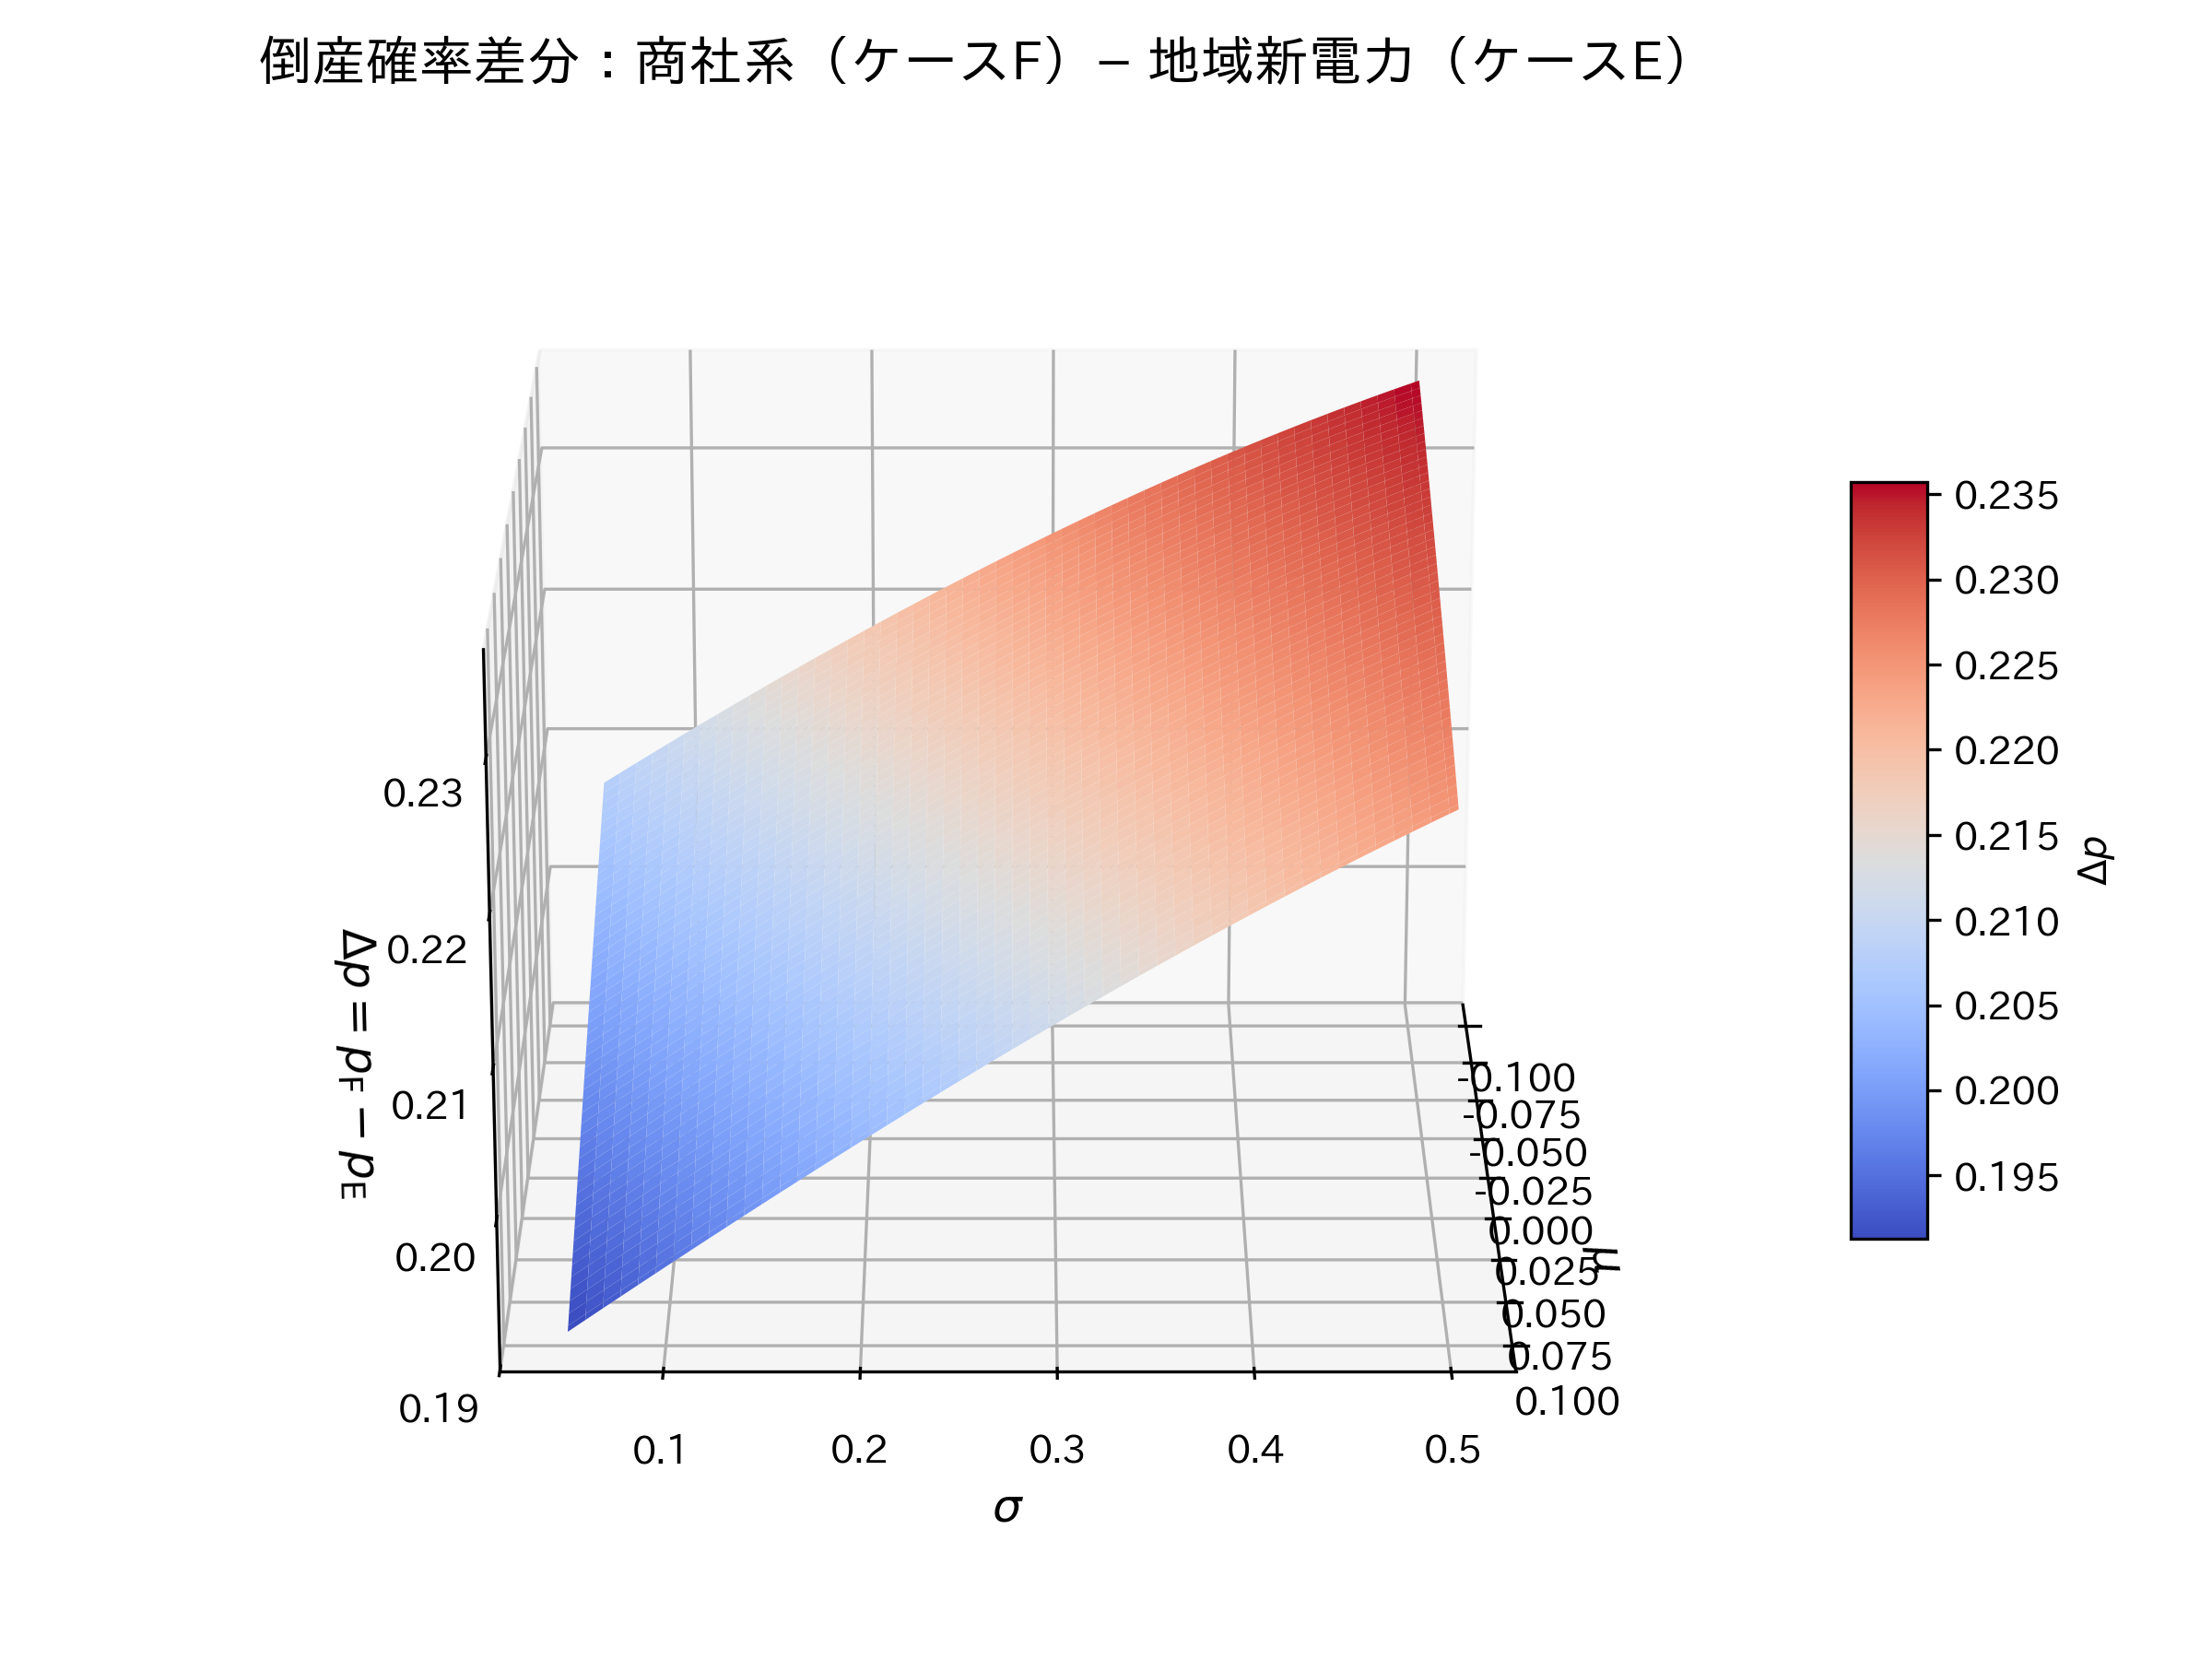
\includegraphics[width=0.75\linewidth]{figures/surface_diff_F_minus_E.png}
    \caption{倒産確率の差分サーフェス：商社系（ケースF）$-$ 地域新電力（ケースE）}
    \label{fig:surface_diff_F_minus_E}
\end{figure}

図\ref{fig:surface_diff_F_minus_E} に示すとおり，
$\Delta p$ は全域で正となり，
商社系（ケースF）の倒産確率が地域新電力（ケースE）より一貫して低いことが確認できる。
特に以下の3点が重要である。

\begin{enumerate}
    \item \textbf{市場ショックが大きいほど格差が拡大する}  
    $\sigma$ が大きい領域では $\Delta p$ が急速に増加しており，
    市場変動に対する耐性が支援能力 $S$ の差によって大きく左右されることがわかる。

    \item \textbf{収益性が低いほど支援能力の効果が強く現れる}  
    $\mu$ が負の領域では $\Delta p$ が最大化し，
    収益性の低下が地域新電力の倒産確率を大きく押し上げる一方，
    商社系は支援能力 $S=2$ により倒産確率の上昇が抑制される。

    \item \textbf{支援能力 $S$ の上昇は，中規模企業においても倒産確率を大幅に低減する}  
    ケースEとケースFの差分は 0.2〜0.3 程度であり，
    大企業と地方電力の比較（0.6〜0.7）ほど極端ではないものの，
    中規模企業においても支援能力が倒産確率に与える影響は決定的である。
\end{enumerate}

以上の結果は，
「企業規模が小さいほど倒産しやすい」という単純な構図ではなく，
\textbf{支援能力 $S$ が部分的にでも確保されれば，
中規模企業であっても倒産リスクを大幅に低減できる}
ことを示している。
すなわち，地域新電力の生存可能性は，


\[
(\mu,\ \sigma,\ D) \text{ に加えて } S \text{ をいかに確保できるか}
\]


に強く依存しており，
自治体・地銀・地域企業との連携やスポンサー支援の獲得が
実務的な生存戦略として極めて重要である。




% ============================================================
\subsection{ケース横断的な比較と含意}
% ------------------------------------------------------------
% ・ケースA〜Fの共通点と相違点を体系的に整理する
% ・S と D の影響を統合的に評価する
% ・第7章の実証分析への橋渡しを行う
% ------------------------------------------------------------

ケースA〜Fの比較から，以下の統合的な特徴が確認される。

\begin{itemize}
    \item 支援能力 $S$ の上昇は，倒産確率の地形全体を右方へ移動させ，
          外生ショックに対する耐性を高める。
    \item 負債比率 $D$ の上昇は，倒産確率の立ち上がりを急峻にし，
          高ボラティリティ環境での脆弱性を増幅する。
    \item 収益性 $\mu$ の改善効果は，負債比率が高い企業ほど大きく，
          財務的に脆弱な企業ほど収益性の改善が倒産確率低下に直結する。
\end{itemize}

これらの特徴は，第4章で導出した理論モデルの符号条件と整合的であるだけでなく，
新電力企業の倒産事例で指摘されてきたリスク要因
（収益性の低下，外生ショック，スポンサー支援の有無，負債過多）
を構造的に再現している。
次章では，これらの理論的含意を踏まえつつ，
実際の財務データを用いた実証分析を行い，
$Z_{\text{lin}}$ の予測性能と現実的な適用可能性を検証する。

% ============================================================
% 7.7 B&S 型倒産リスクシミュレーション
% ------------------------------------------------------------
% ・B&S 型ロジット式に基づき，新電力の代表パターンごとの倒産確率を算出
% ・第6章前半の Merton 型シミュレーションと比較し，リスク構造の整合性を確認
% ・第7章の実証分析で用いる B&S 型モデルの直感的含意を整理
% ============================================================

\section{B\&S 型倒産リスクシミュレーション}
\label{sec:bs_risk_simulation}

本節では，Bharath and Shumway（2008）に代表される reduced-form 型の
倒産確率モデルを，新電力企業の文脈に適用した場合の挙動をシミュレーションにより確認する。
具体的には，第5章で定義した収益性 $\mu$，市場ショック $\sigma$，
支援能力 $S$，負債比率 $D$ を説明変数とする B\&S 型ロジット式を用いて，
第6章前半で設定した新電力の代表的な財務プロファイル（ケースA〜F）ごとに
倒産確率を算出し，Merton 型シミュレーションの結果と比較する。

この分析の目的は，第7章で用いる B\&S 型ロジットモデルが，
Merton 型理論モデルと同様のリスク構造（$\mu$，$\sigma$，$S$，$D$ の符号条件や
相対的重要度）を再現しているかを確認し，
実証分析におけるモデル選択の直感的な裏付けを与えることである。

% ------------------------------------------------------------
\subsection{B\&S 型ロジットモデルの仕様}

本節で用いる倒産確率モデルは，次のロジット形式で与えられる。



\[
\text{logit}(p_i)
= \alpha + \beta_{\mu} \mu_i + \beta_{\sigma} \sigma_i
  + \beta_{S} S_i + \beta_{D} D_i,
\]





\[
p_i = \frac{1}{1 + \exp\bigl(-\{\alpha + \beta_{\mu} \mu_i
  + \beta_{\sigma} \sigma_i + \beta_{S} S_i + \beta_{D} D_i\}\bigr)}.
\]



係数は，第4章および第6章前半で確認した符号条件と整合的になるように設定する。



\[
\alpha = 0.0,\quad
\beta_{\mu} = -4.0,\quad
\beta_{\sigma} = 3.0,\quad
\beta_{S} = -0.8,\quad
\beta_{D} = 2.0.
\]



% ------------------------------------------------------------
\subsection{新電力の代表ケースの設定}

第6章前半と同様に，新電力企業の典型的な財務状態を反映した
6つの代表ケース（A〜F）を用いる。

\begin{itemize}
    \item ケースA：$D=0.3,\ S=0$（独立系・財務健全）
    \item ケースB：$D=0.3,\ S=3$（大手系・財務健全）
    \item ケースC：$D=0.8,\ S=0$（独立系・負債過多）
    \item ケースD：$D=0.8,\ S=3$（大手系・負債過多）
    \item ケースE：$D=0.5,\ S=1$（地域新電力）
    \item ケースF：$D=0.5,\ S=2$（商社系）
\end{itemize}

収益性 $\mu$ と市場ショック $\sigma$ は以下の範囲で連続的に変化させる。



\[
\mu \in [-0.10, 0.10],\qquad
\sigma \in [0.05, 0.50].
\]



% ------------------------------------------------------------
\subsection{倒産確率サーフェスの可視化}

以下では，ケースA〜Fについて，
B\&S 型ロジットモデルに基づく倒産確率サーフェスを示す。

% ---------- ケースA ----------
\subsubsection*{ケースA：$D=0.3,\ S=0$（独立系・財務健全）}

\begin{figure}[H]
    \centering
    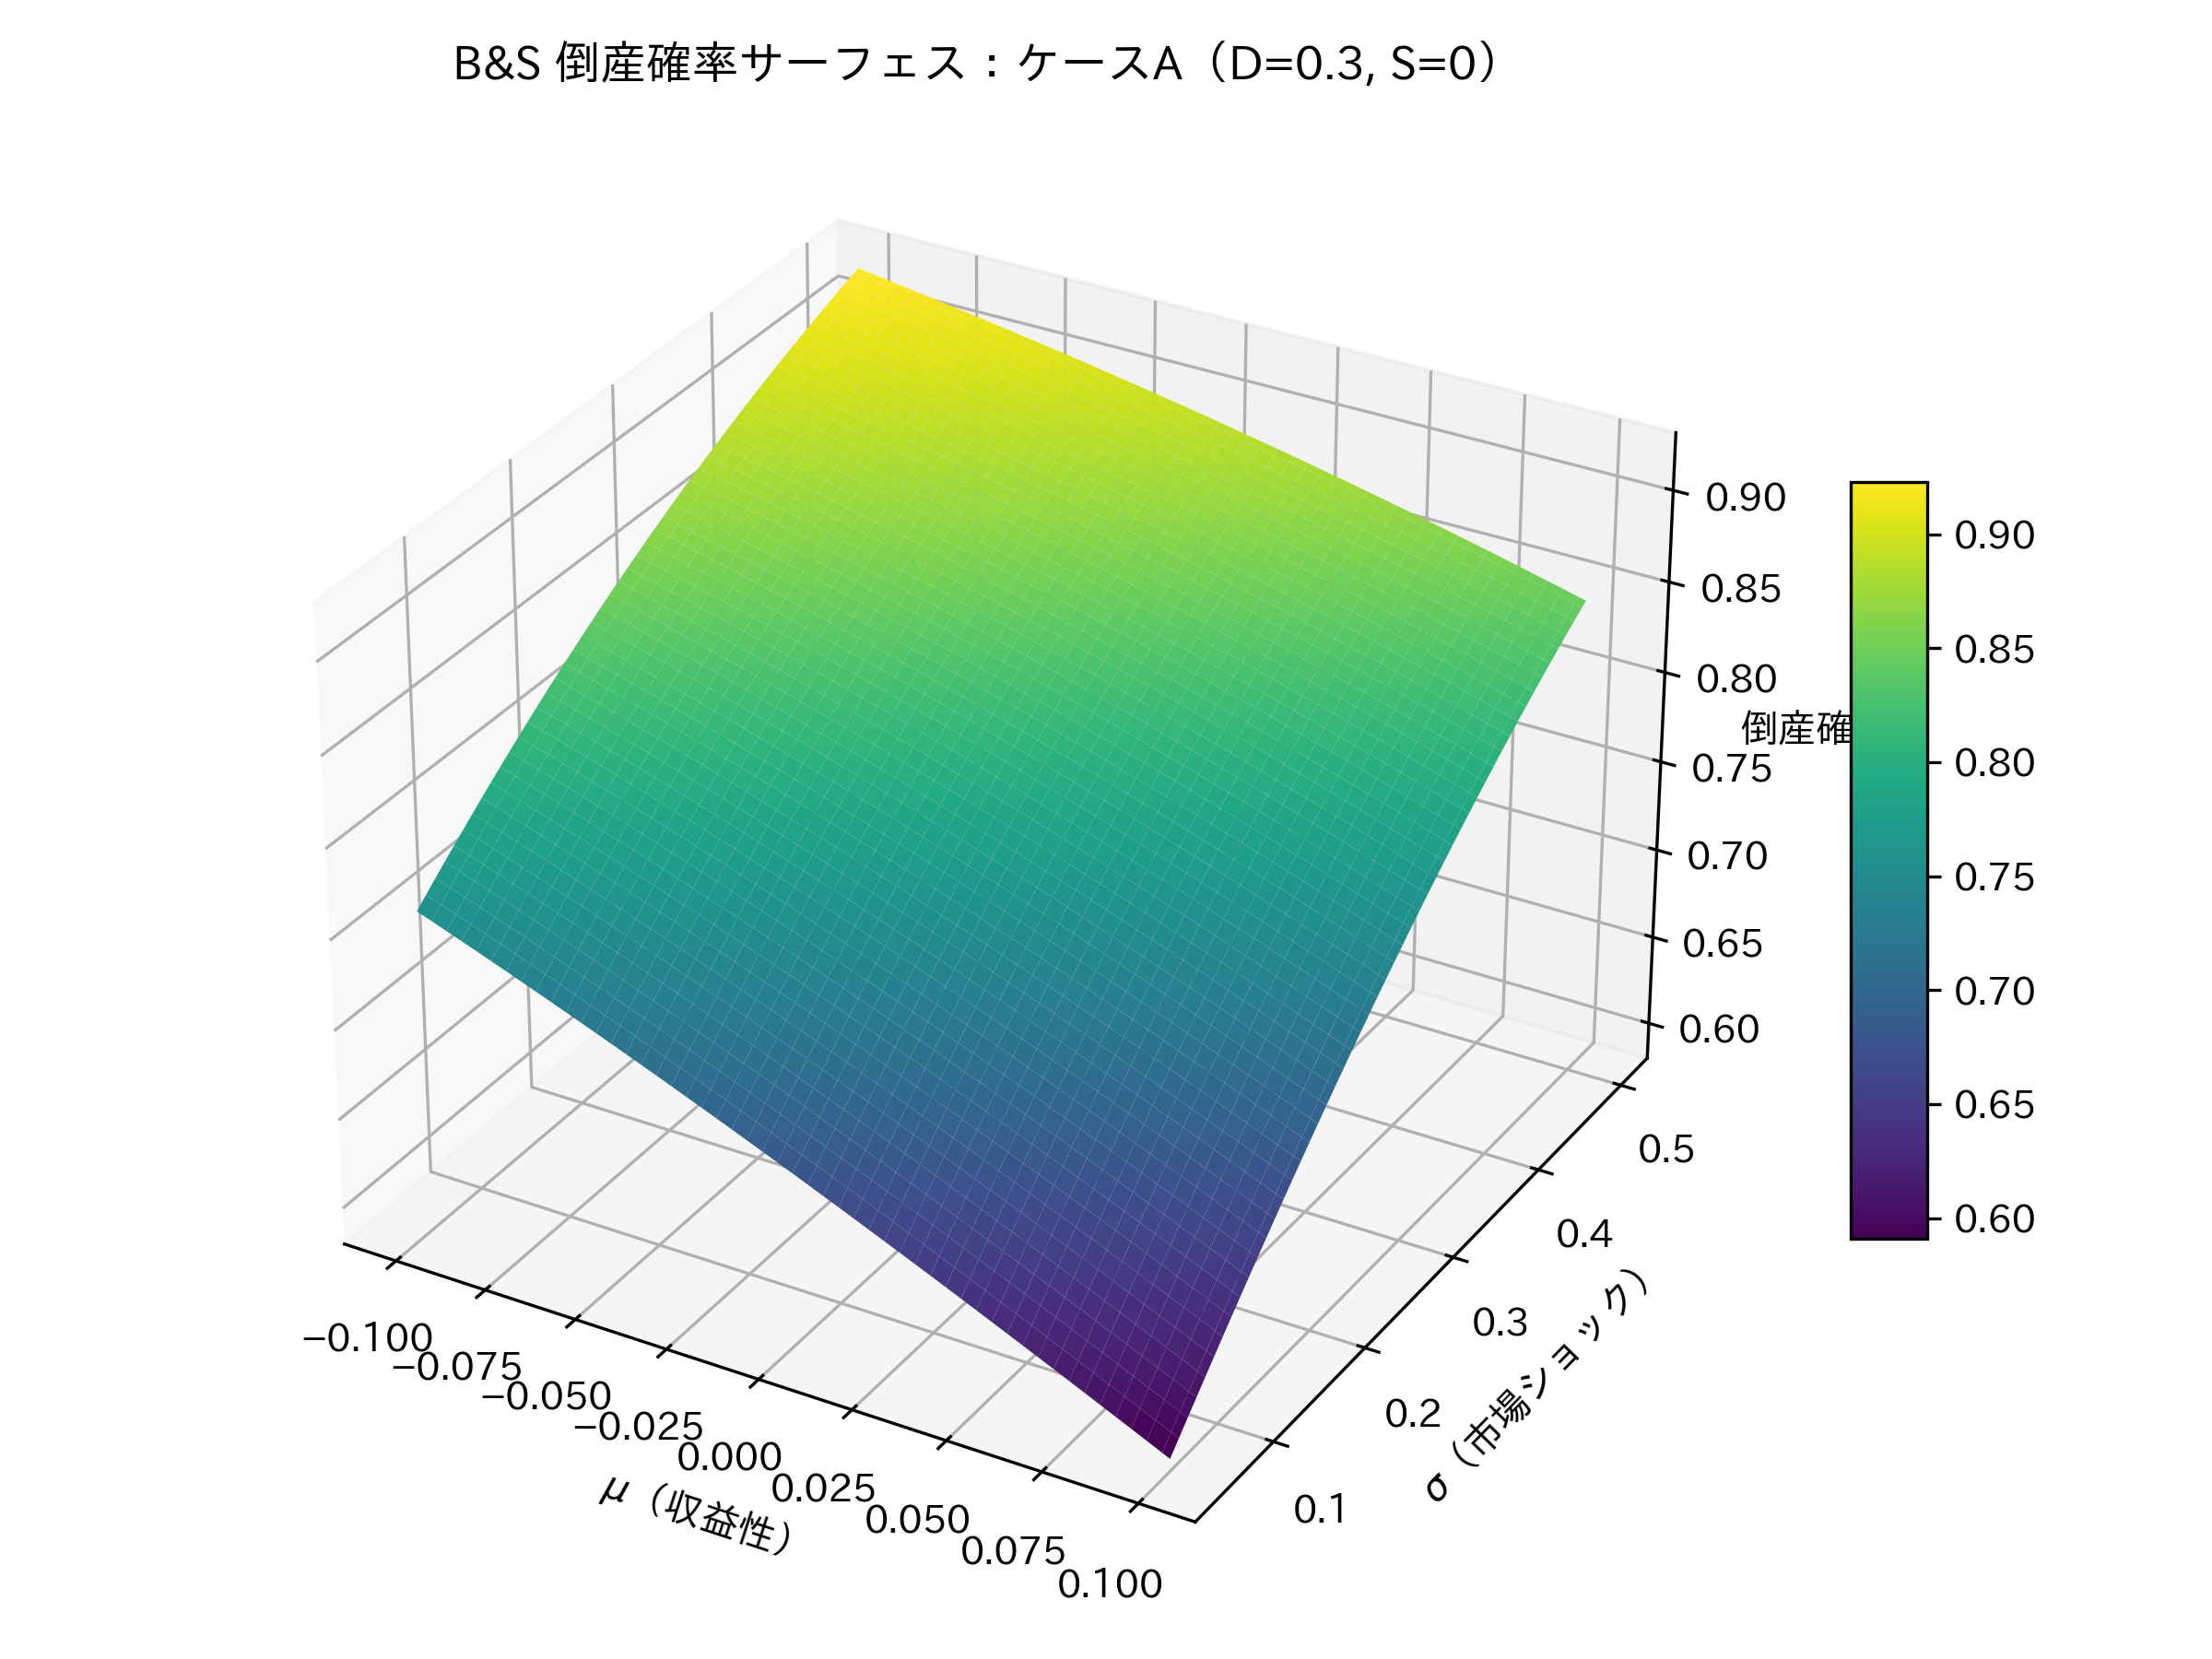
\includegraphics[width=0.75\linewidth]{figures/bs_surface_caseA.png}
    \caption{B\&S 型倒産確率サーフェス：ケースA（独立系・財務健全）}
    \label{fig:bs_surface_caseA}
\end{figure}

% ---------- ケースB ----------
\subsubsection*{ケースB：$D=0.3,\ S=3$（大手系・財務健全）}

\begin{figure}[H]
    \centering
    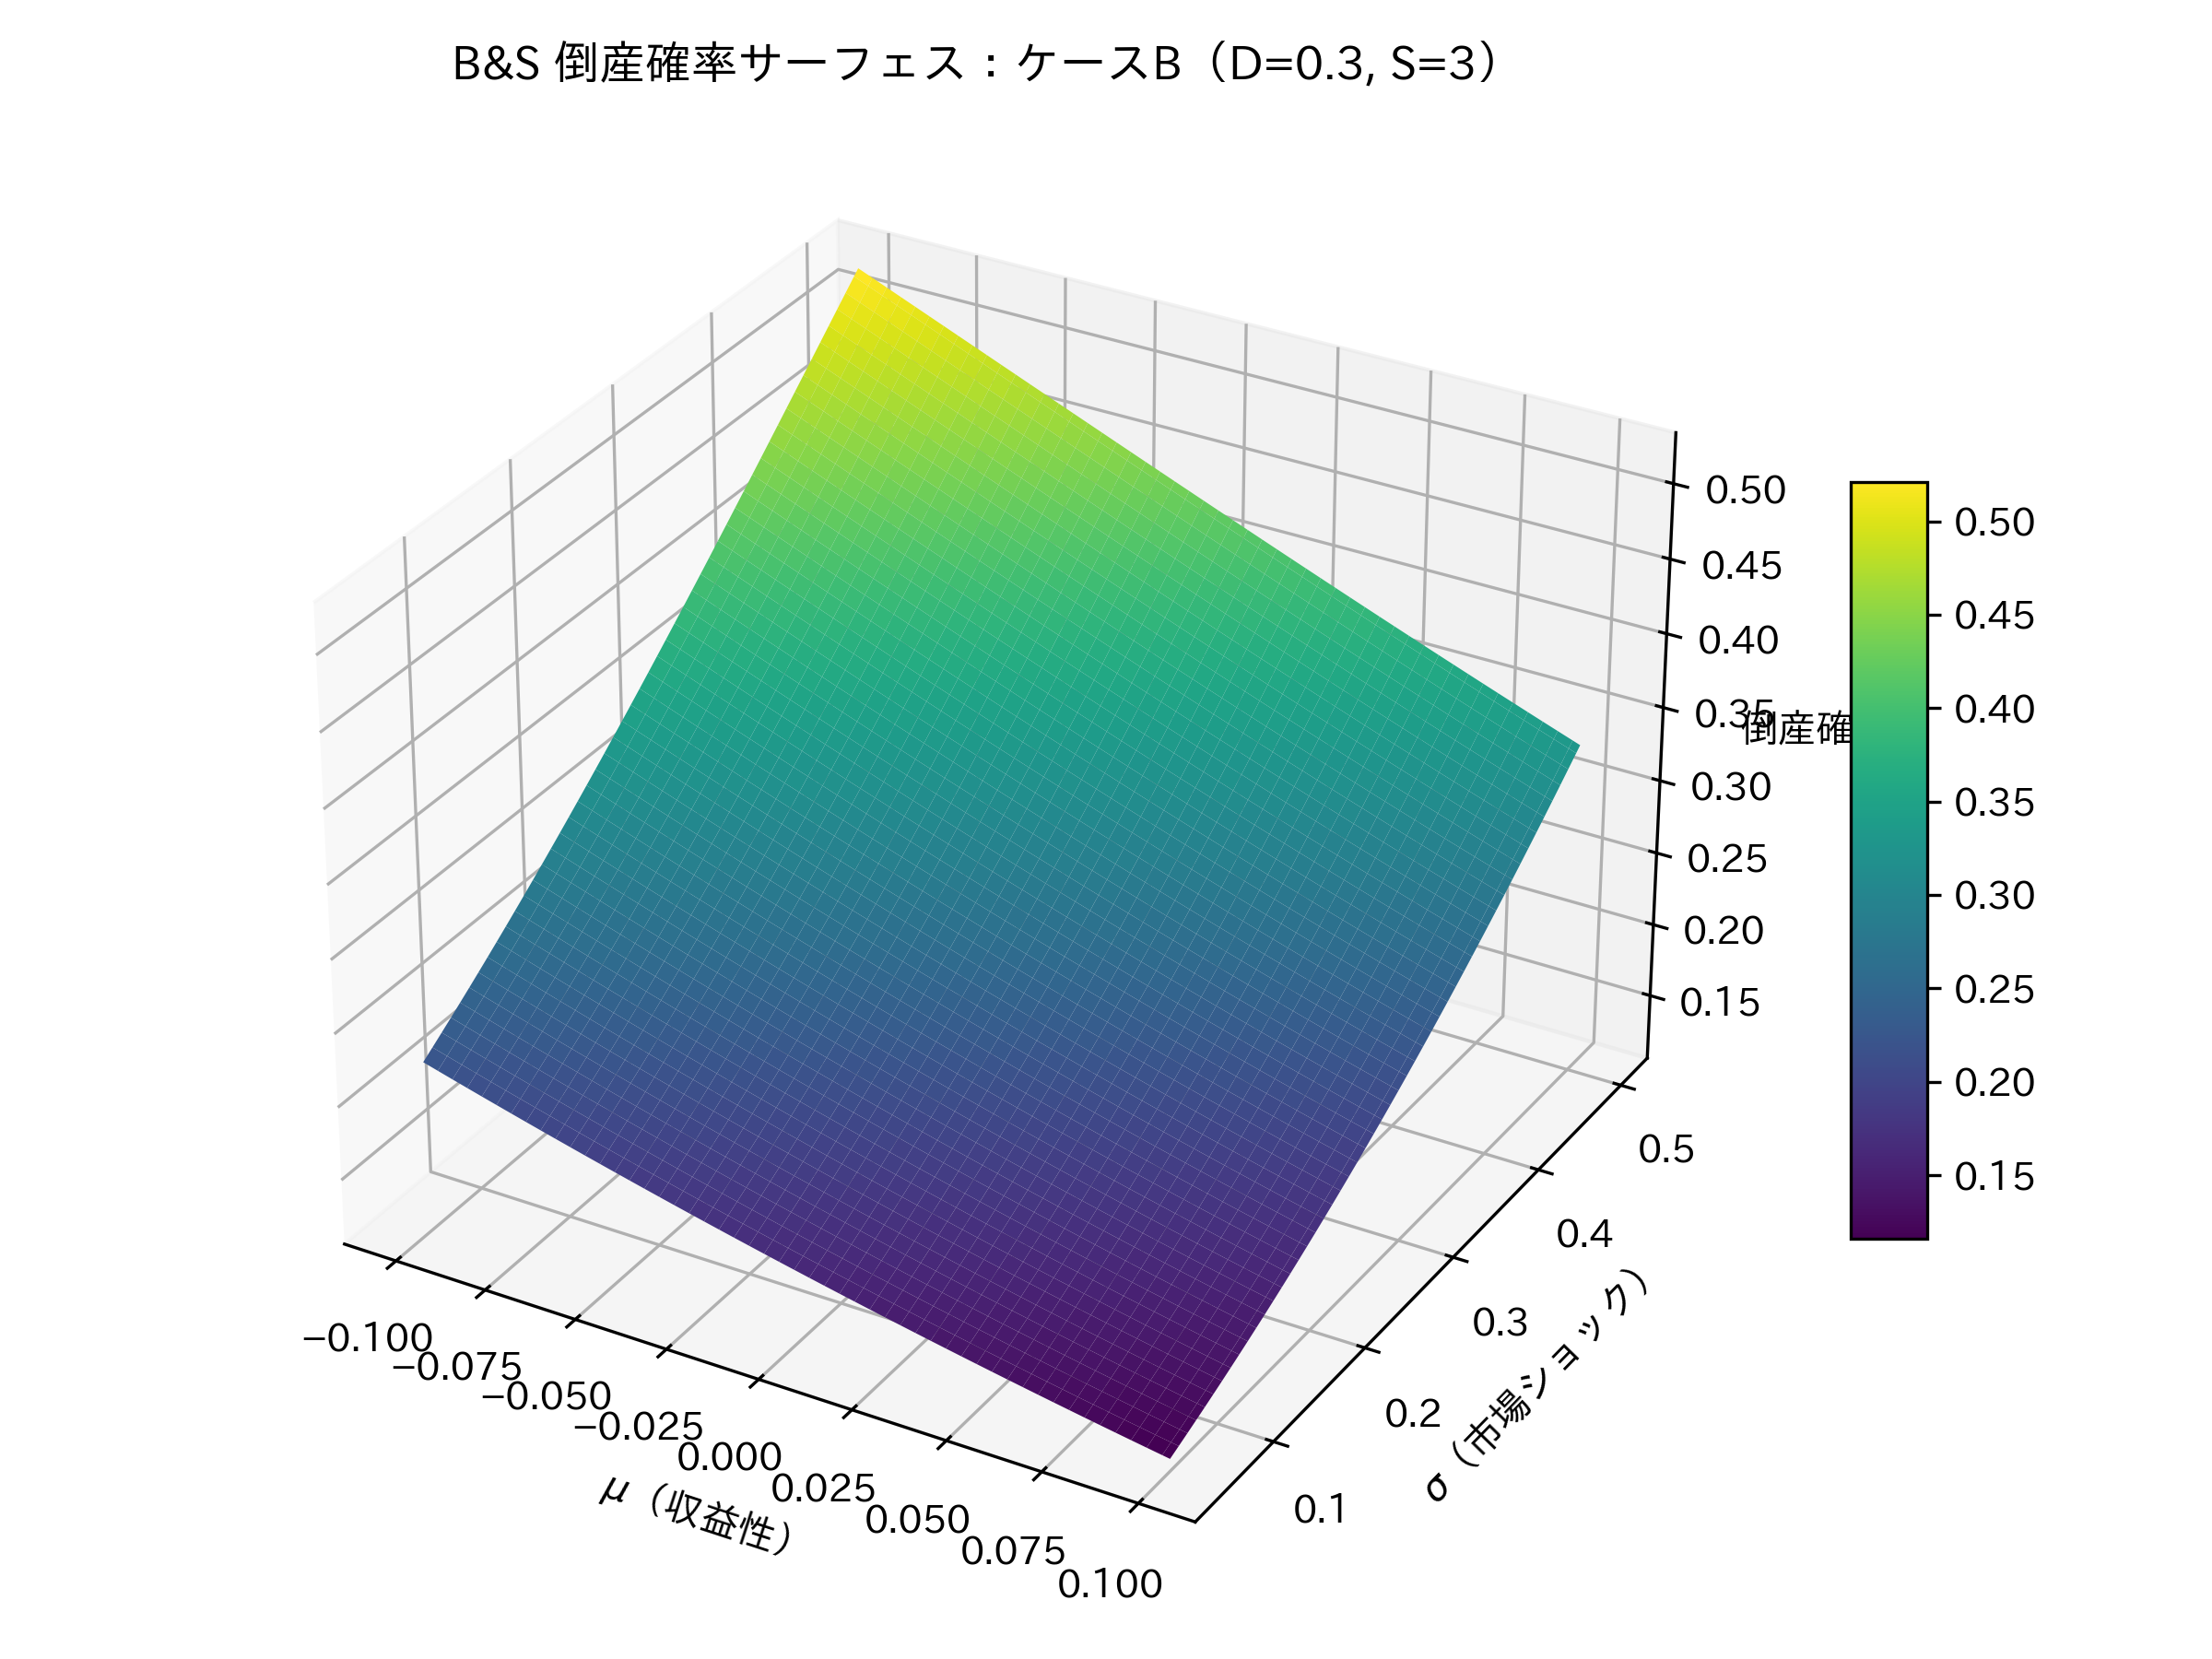
\includegraphics[width=0.75\linewidth]{figures/bs_surface_caseB.png}
    \caption{B\&S 型倒産確率サーフェス：ケースB（大手系・財務健全）}
    \label{fig:bs_surface_caseB}
\end{figure}

% ---------- ケースC ----------
\subsubsection*{ケースC：$D=0.8,\ S=0$（独立系・負債過多）}

\begin{figure}[H]
    \centering
    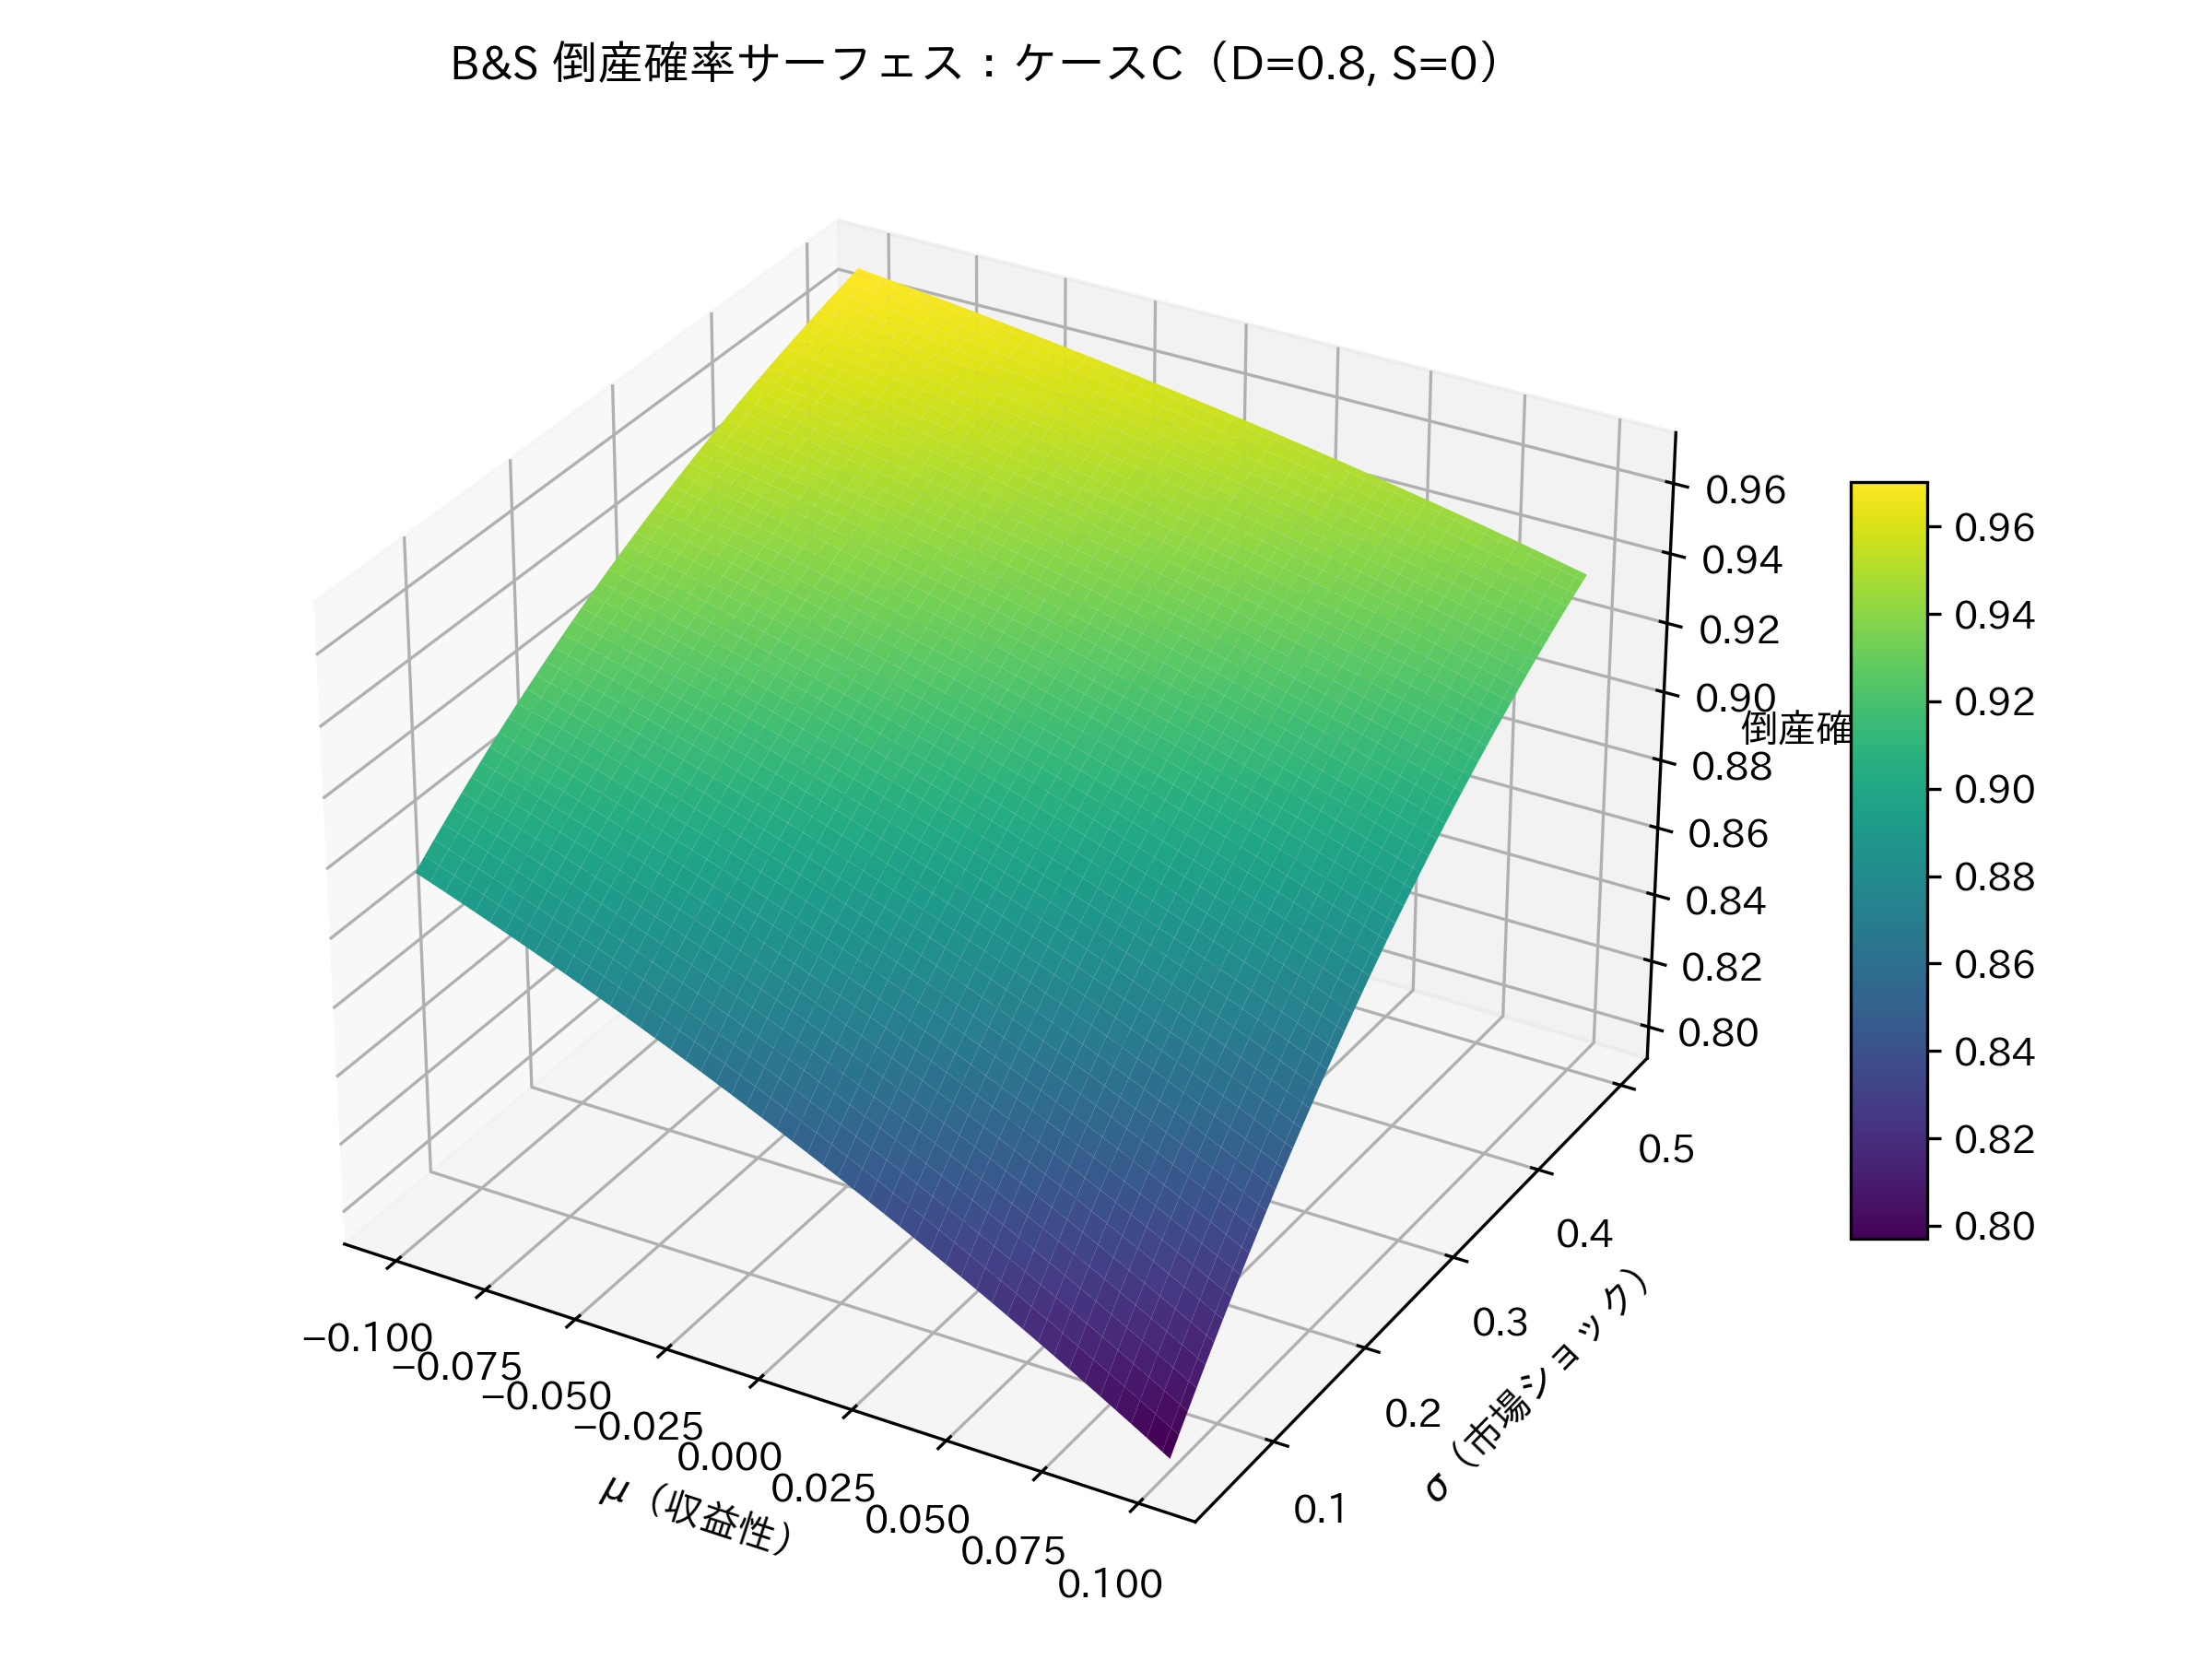
\includegraphics[width=0.75\linewidth]{figures/bs_surface_caseC.png}
    \caption{B\&S 型倒産確率サーフェス：ケースC（独立系・負債過多）}
    \label{fig:bs_surface_caseC}
\end{figure}

% ---------- ケースD ----------
\subsubsection*{ケースD：$D=0.8,\ S=3$（大手系・負債過多）}

\begin{figure}[H]
    \centering
    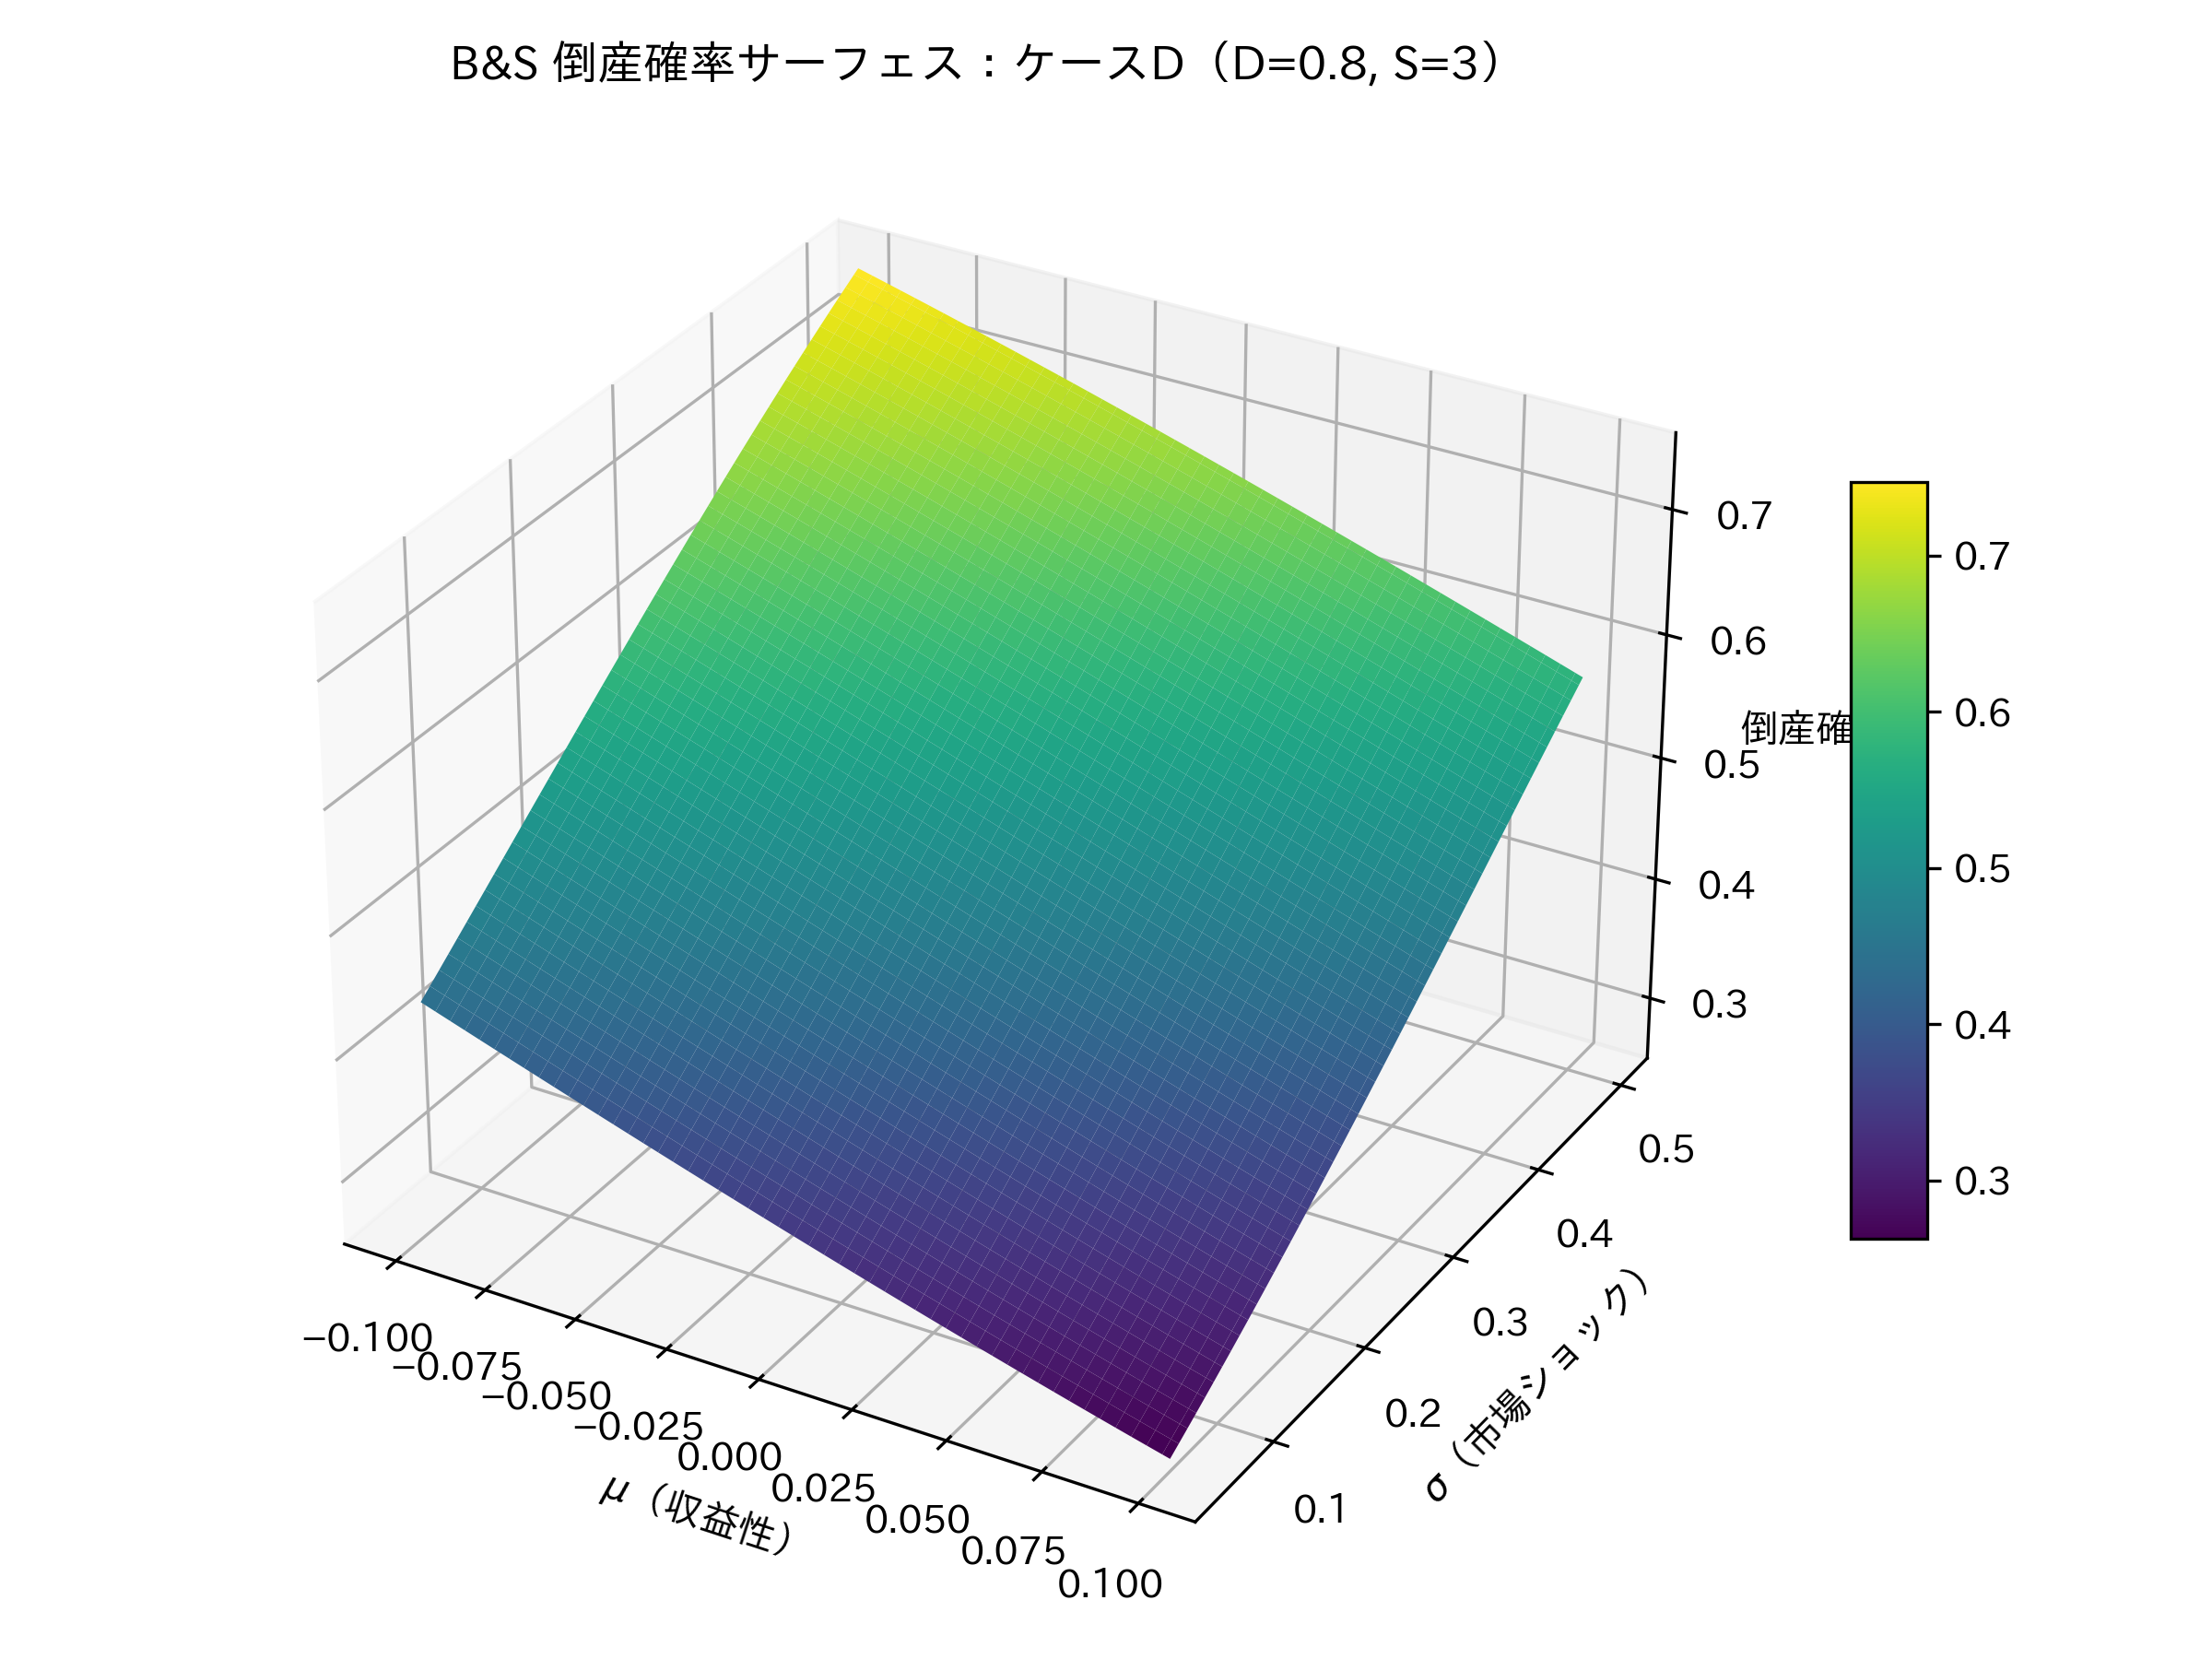
\includegraphics[width=0.75\linewidth]{figures/bs_surface_caseD.png}
    \caption{B\&S 型倒産確率サーフェス：ケースD（大手系・負債過多）}
    \label{fig:bs_surface_caseD}
\end{figure}

% ---------- ケースE ----------
\subsubsection*{ケースE：$D=0.5,\ S=1$（地域新電力）}

\begin{figure}[H]
    \centering
    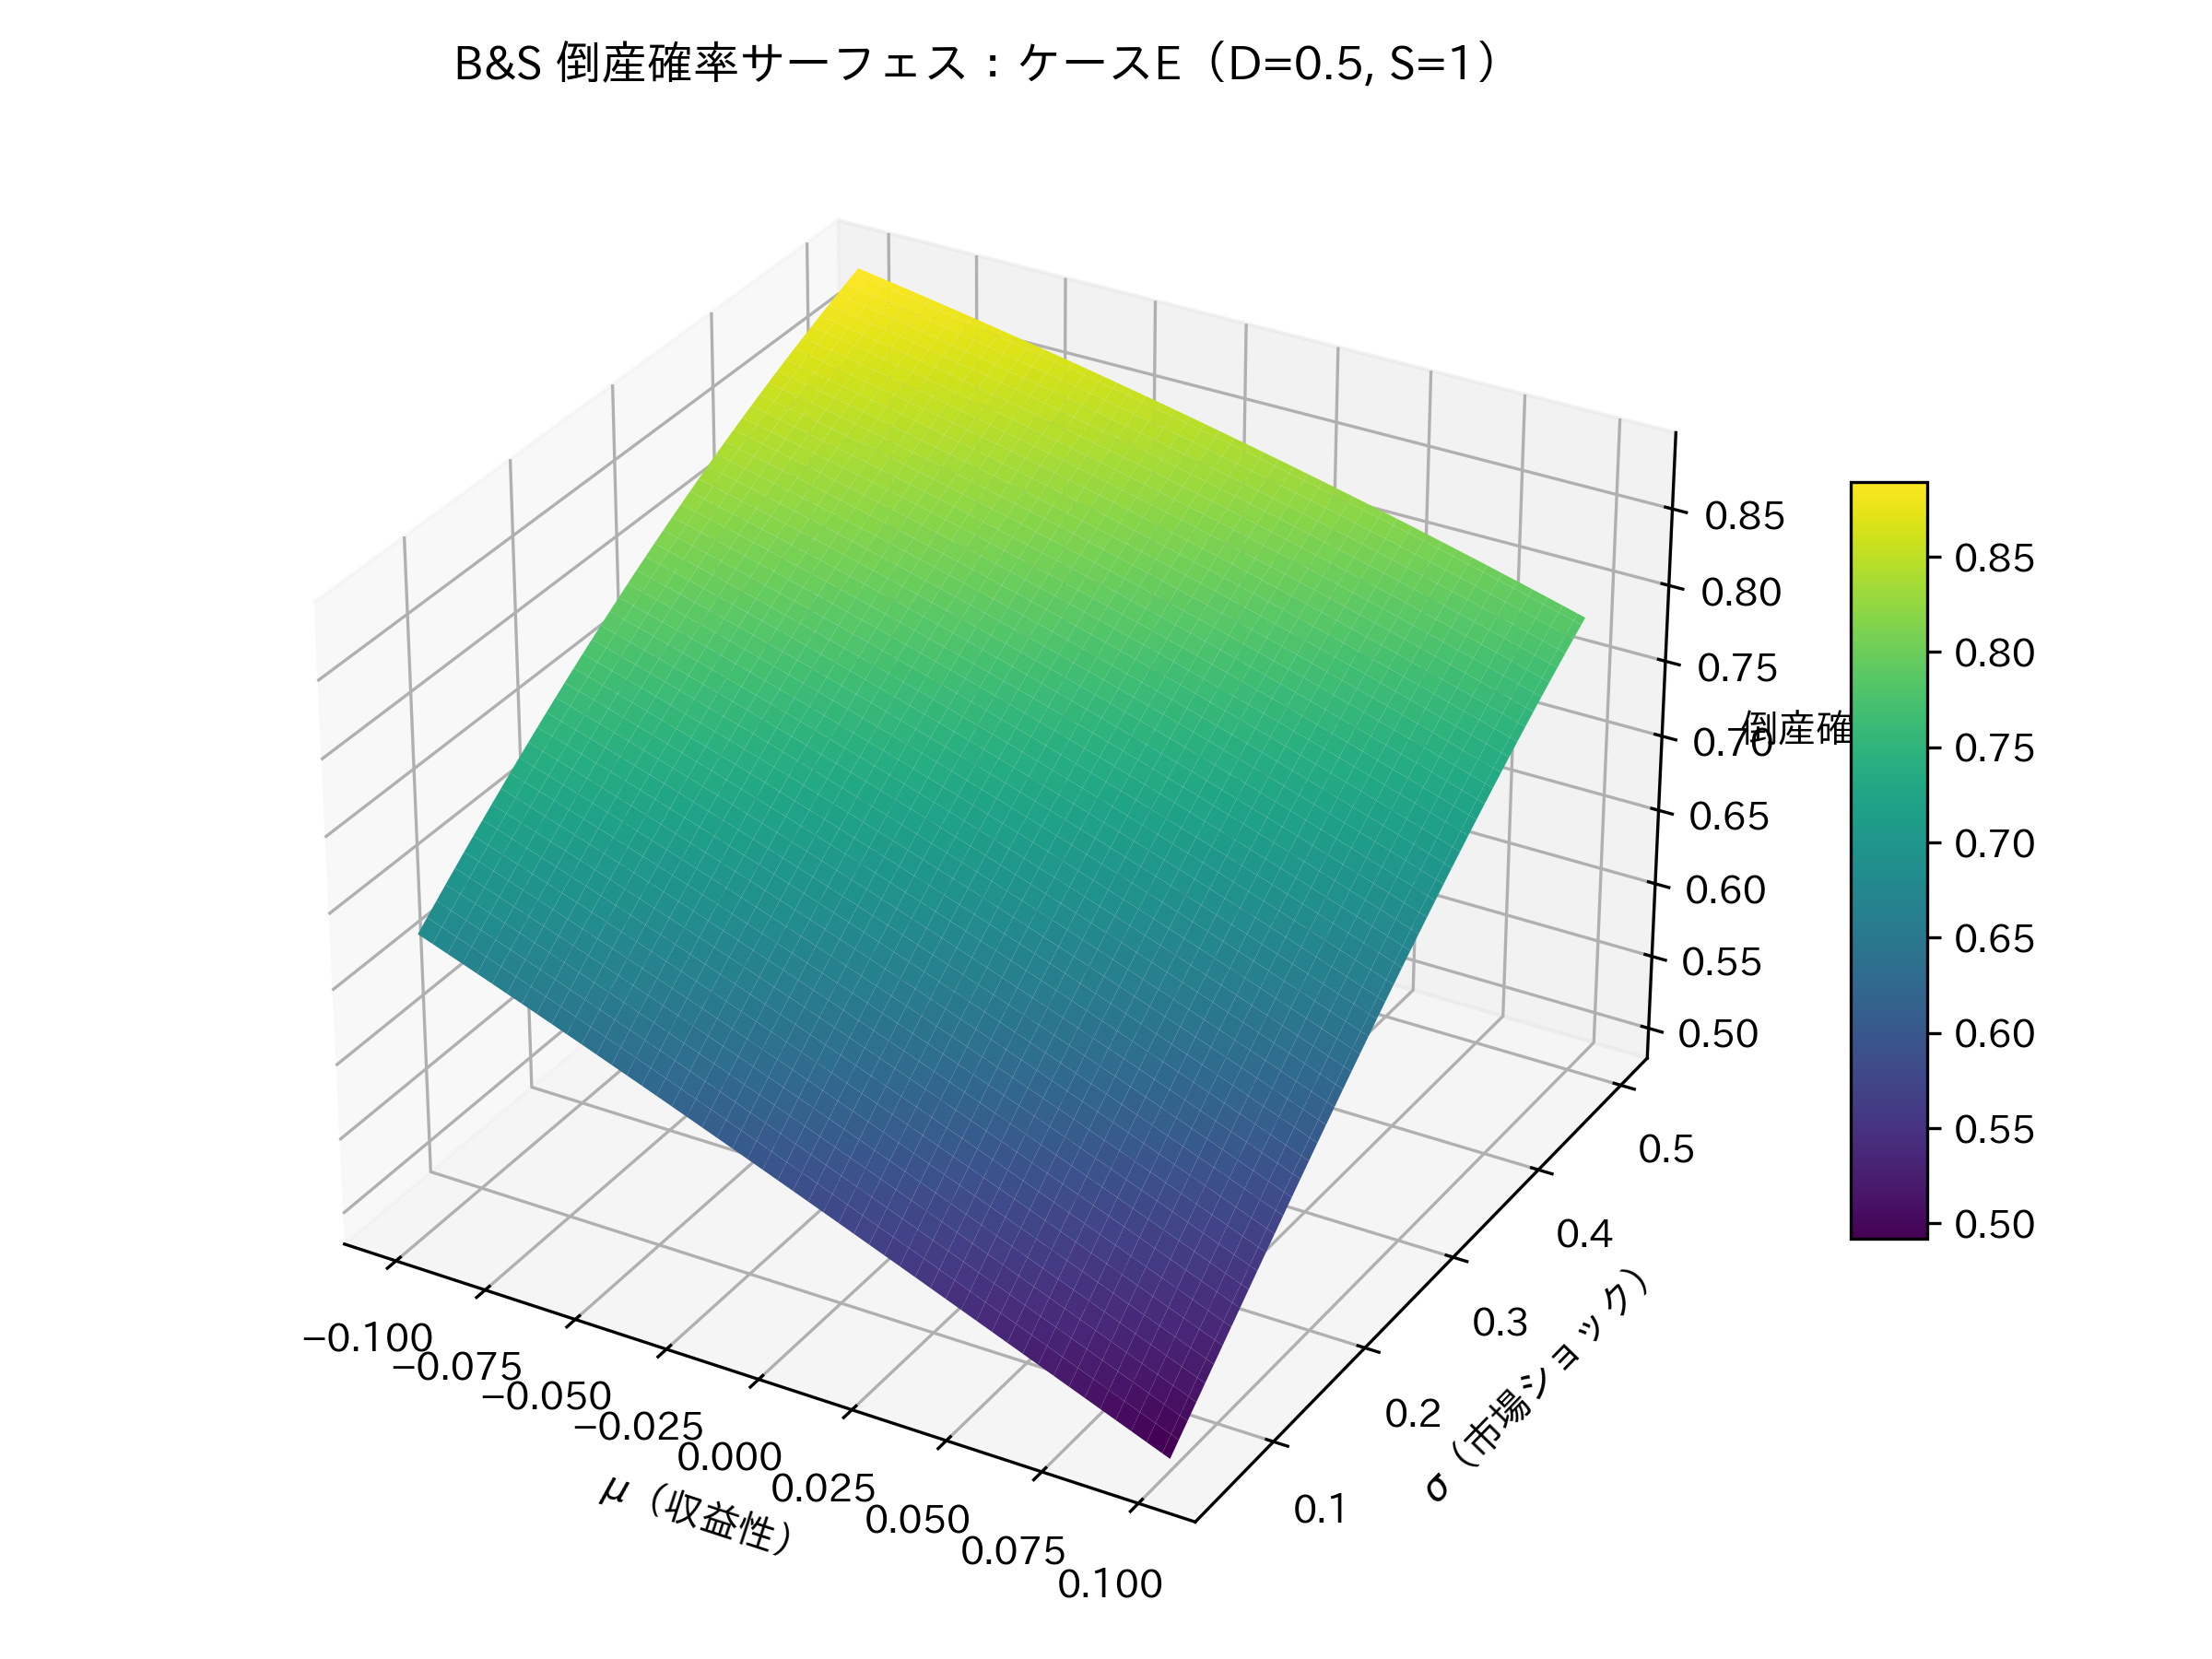
\includegraphics[width=0.75\linewidth]{figures/bs_surface_caseE.png}
    \caption{B\&S 型倒産確率サーフェス：ケースE（地域新電力）}
    \label{fig:bs_surface_caseE}
\end{figure}

% ---------- ケースF ----------
\subsubsection*{ケースF：$D=0.5,\ S=2$（商社系）}

\begin{figure}[H]
    \centering
    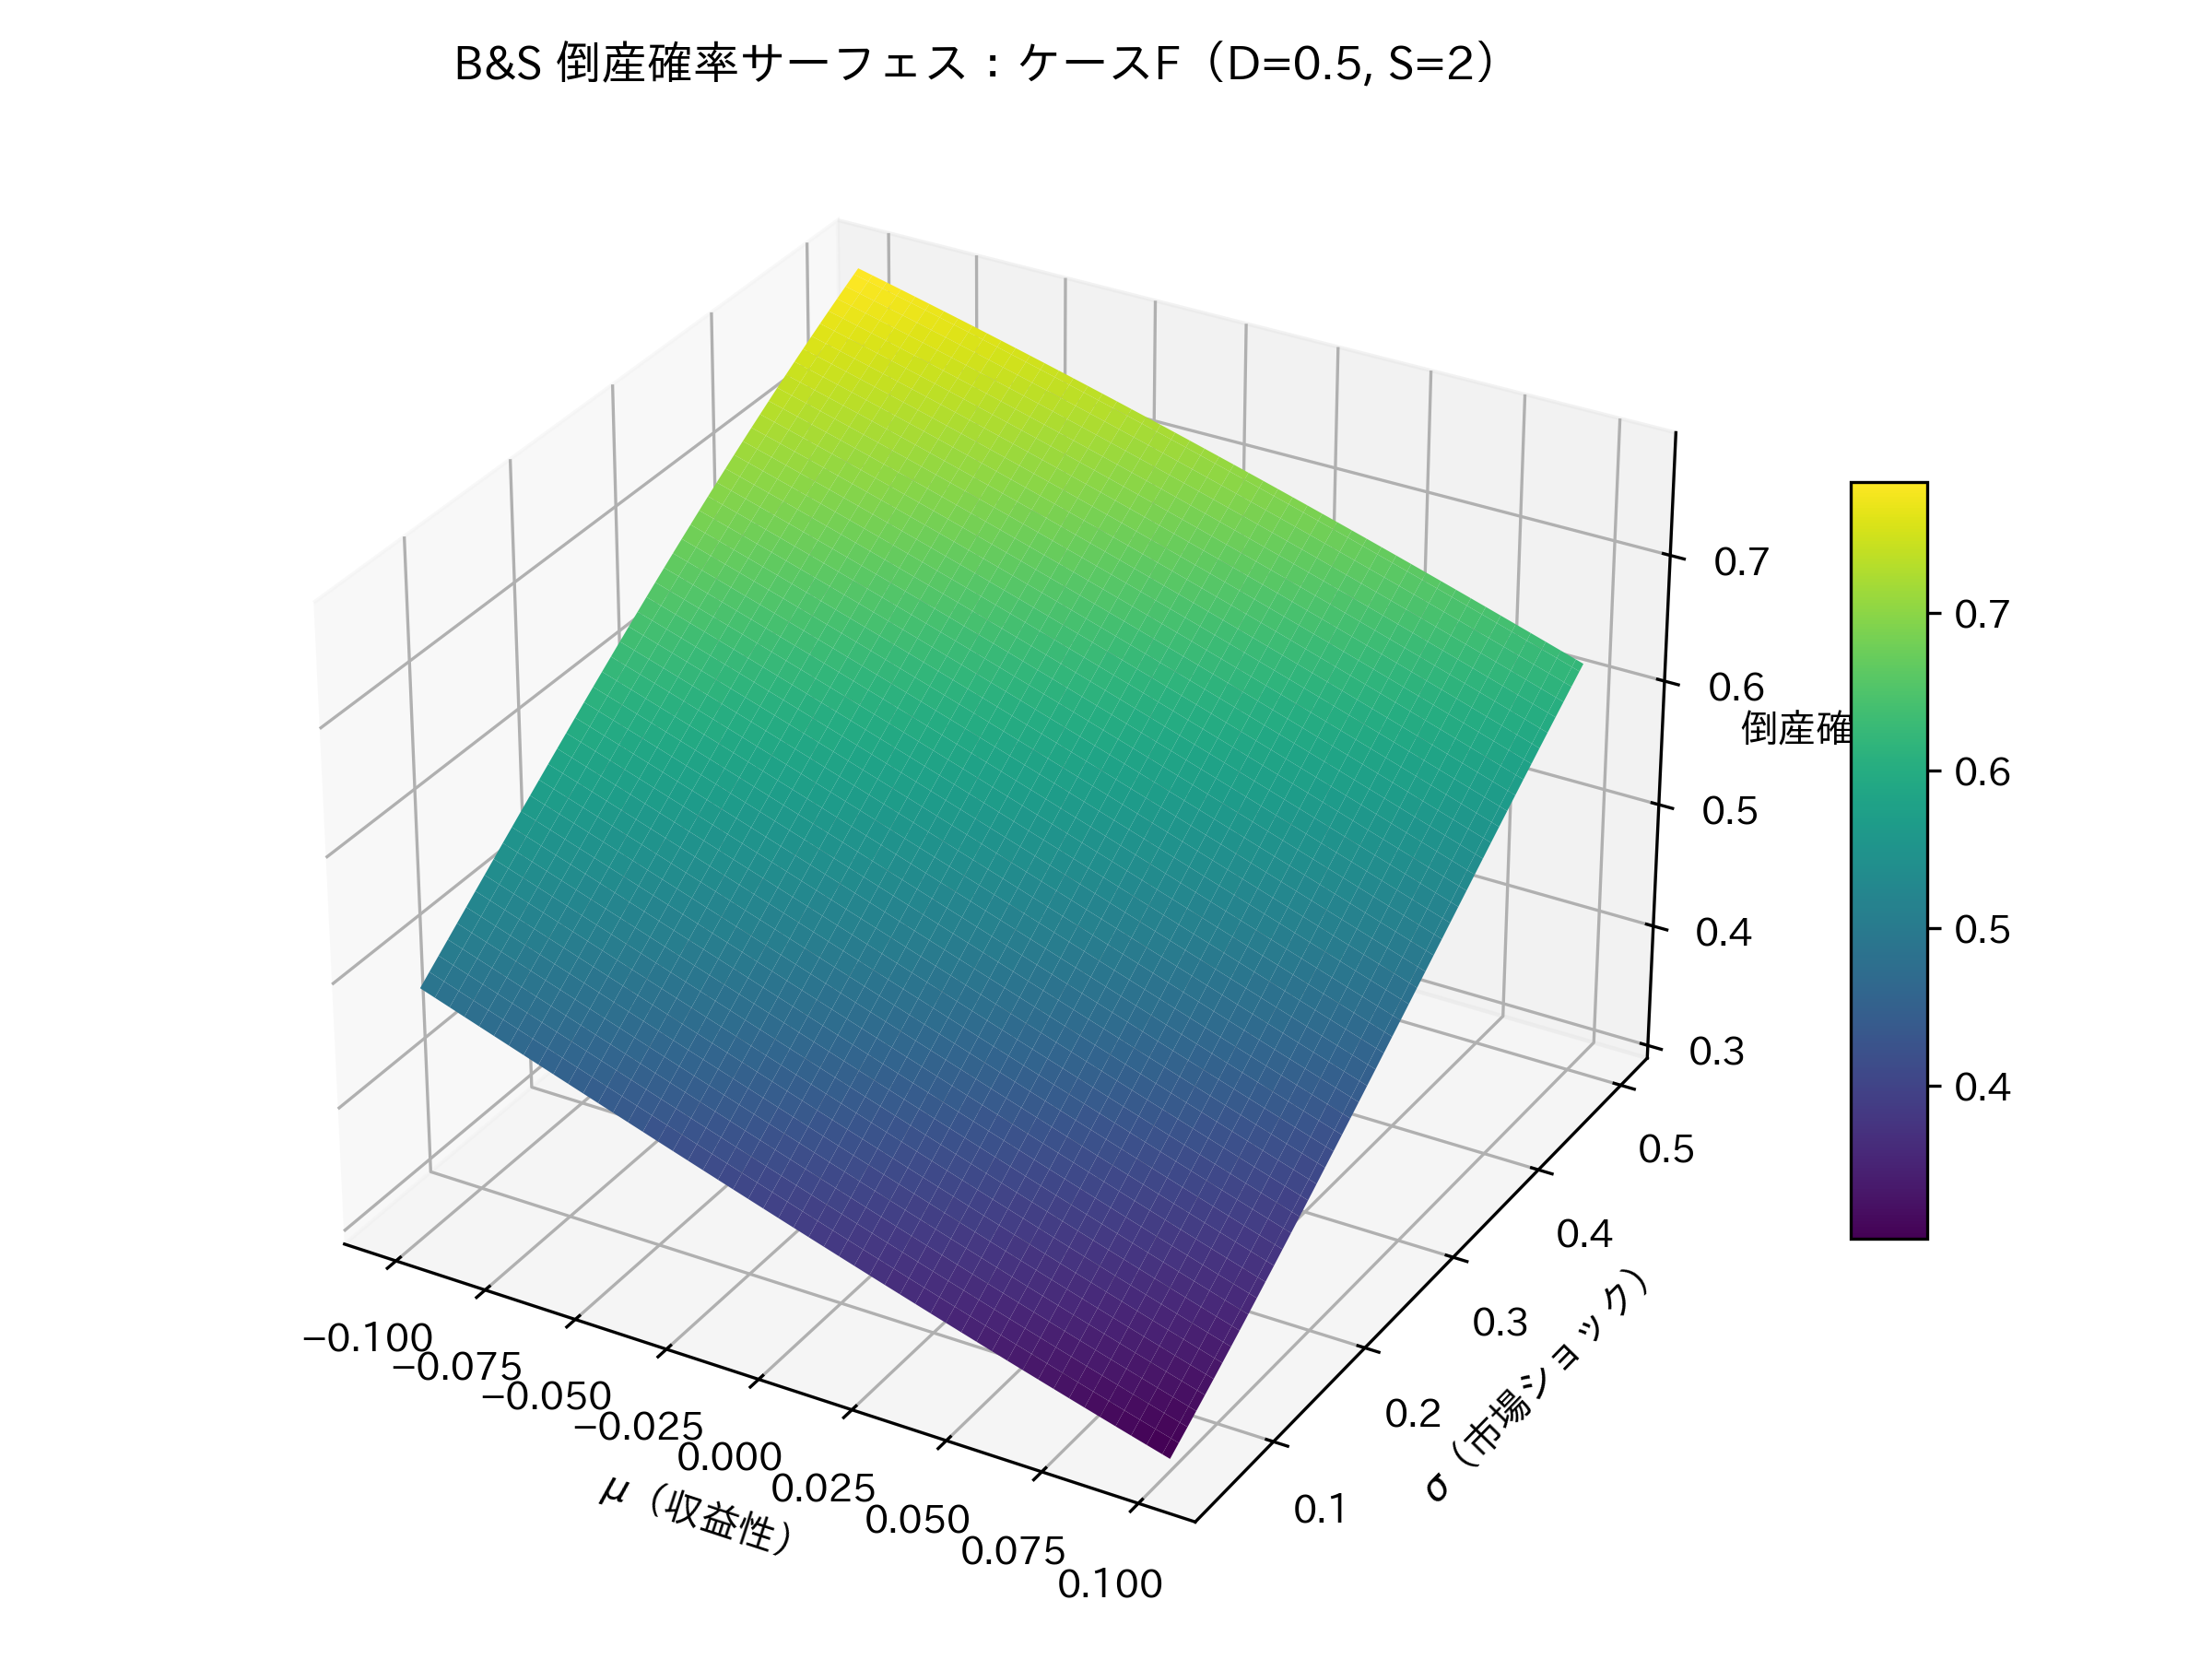
\includegraphics[width=0.75\linewidth]{figures/bs_surface_caseF.png}
    \caption{B\&S 型倒産確率サーフェス：ケースF（商社系）}
    \label{fig:bs_surface_caseF}
\end{figure}

% ------------------------------------------------------------
\subsection{Merton 型シミュレーションとの整合性}

B\&S 型ロジットモデルは企業価値プロセスを明示的に扱わない reduced-form モデルであるが，
上記のサーフェス比較から，以下の点が確認される。

\begin{itemize}
    \item $\mu$ の上昇は倒産確率を低下させる。
    \item $\sigma$ の上昇は倒産確率を上昇させる。
    \item 支援能力 $S$ が高いほど倒産確率は低下する。
    \item 負債比率 $D$ が高いほど倒産確率は急激に上昇する。
\end{itemize}

これらは第6章前半の Merton 型シミュレーションと同じ方向性を示しており，
両モデルが新電力企業の倒産リスク構造について
共通の含意を持つことを示している。

% ------------------------------------------------------------
\subsection{本節の含意と第8章への橋渡し}

本節の B\&S 型倒産リスクシミュレーションにより，
Merton 型理論モデルと B\&S 型ロジットモデルが，
新電力企業の倒産リスクを規定する主要因
（収益性 $\mu$，市場ショック $\sigma$，支援能力 $S$，負債比率 $D$）
について整合的な構造を持つことが確認された。

すなわち，B\&S 型ロジットモデルは，
Merton 型理論モデルが示す倒産確率の符号条件や相対的重要度を
現実データの枠組みで実装したものであり，
第8章で構築する潜在倒産距離モデルの妥当性を理論的に補強する役割を果たす。

さらに，本章で示した倒産確率サーフェスおよびケース間の差分サーフェスは，
新電力企業の財務構造の違いが倒産確率にどのように反映されるかを
視覚的かつ体系的に把握するためのものであり，
本研究における重要な理論的アウトプットのひとつである。

一方，\textbf{proxy 変数（A〜D）の精度が推定係数や倒産確率の識別性能に与える影響を
理想化された世界で評価する proxy 妥当性シミュレーションは，
本章の構造分析を計量的に補完するものであり，
その詳細は付録Cにまとめている}。
これにより，第8章の潜在倒産距離モデルおよび第9章の Ordered Logit 推定に先立ち，
proxy の妥当性と限界を理論的に裏付けることができる。

以上より，本章は，
\textbf{理論モデル（第4章）→ シミュレーション分析（第7章）→ 潜在倒産距離モデル（第8章）→ Ordered Logit 実証分析（第9章）}
という本研究の一連の流れの中で，
理論編と実証編を接続する重要な役割を果たす。

